% Options for packages loaded elsewhere
\PassOptionsToPackage{unicode}{hyperref}
\PassOptionsToPackage{hyphens}{url}
%
\documentclass[
]{book}
\usepackage{amsmath,amssymb}
\usepackage{iftex}
\ifPDFTeX
  \usepackage[T1]{fontenc}
  \usepackage[utf8]{inputenc}
  \usepackage{textcomp} % provide euro and other symbols
\else % if luatex or xetex
  \usepackage{unicode-math} % this also loads fontspec
  \defaultfontfeatures{Scale=MatchLowercase}
  \defaultfontfeatures[\rmfamily]{Ligatures=TeX,Scale=1}
\fi
\usepackage{lmodern}
\ifPDFTeX\else
  % xetex/luatex font selection
\fi
% Use upquote if available, for straight quotes in verbatim environments
\IfFileExists{upquote.sty}{\usepackage{upquote}}{}
\IfFileExists{microtype.sty}{% use microtype if available
  \usepackage[]{microtype}
  \UseMicrotypeSet[protrusion]{basicmath} % disable protrusion for tt fonts
}{}
\makeatletter
\@ifundefined{KOMAClassName}{% if non-KOMA class
  \IfFileExists{parskip.sty}{%
    \usepackage{parskip}
  }{% else
    \setlength{\parindent}{0pt}
    \setlength{\parskip}{6pt plus 2pt minus 1pt}}
}{% if KOMA class
  \KOMAoptions{parskip=half}}
\makeatother
\usepackage{xcolor}
\usepackage{color}
\usepackage{fancyvrb}
\newcommand{\VerbBar}{|}
\newcommand{\VERB}{\Verb[commandchars=\\\{\}]}
\DefineVerbatimEnvironment{Highlighting}{Verbatim}{commandchars=\\\{\}}
% Add ',fontsize=\small' for more characters per line
\usepackage{framed}
\definecolor{shadecolor}{RGB}{248,248,248}
\newenvironment{Shaded}{\begin{snugshade}}{\end{snugshade}}
\newcommand{\AlertTok}[1]{\textcolor[rgb]{0.94,0.16,0.16}{#1}}
\newcommand{\AnnotationTok}[1]{\textcolor[rgb]{0.56,0.35,0.01}{\textbf{\textit{#1}}}}
\newcommand{\AttributeTok}[1]{\textcolor[rgb]{0.13,0.29,0.53}{#1}}
\newcommand{\BaseNTok}[1]{\textcolor[rgb]{0.00,0.00,0.81}{#1}}
\newcommand{\BuiltInTok}[1]{#1}
\newcommand{\CharTok}[1]{\textcolor[rgb]{0.31,0.60,0.02}{#1}}
\newcommand{\CommentTok}[1]{\textcolor[rgb]{0.56,0.35,0.01}{\textit{#1}}}
\newcommand{\CommentVarTok}[1]{\textcolor[rgb]{0.56,0.35,0.01}{\textbf{\textit{#1}}}}
\newcommand{\ConstantTok}[1]{\textcolor[rgb]{0.56,0.35,0.01}{#1}}
\newcommand{\ControlFlowTok}[1]{\textcolor[rgb]{0.13,0.29,0.53}{\textbf{#1}}}
\newcommand{\DataTypeTok}[1]{\textcolor[rgb]{0.13,0.29,0.53}{#1}}
\newcommand{\DecValTok}[1]{\textcolor[rgb]{0.00,0.00,0.81}{#1}}
\newcommand{\DocumentationTok}[1]{\textcolor[rgb]{0.56,0.35,0.01}{\textbf{\textit{#1}}}}
\newcommand{\ErrorTok}[1]{\textcolor[rgb]{0.64,0.00,0.00}{\textbf{#1}}}
\newcommand{\ExtensionTok}[1]{#1}
\newcommand{\FloatTok}[1]{\textcolor[rgb]{0.00,0.00,0.81}{#1}}
\newcommand{\FunctionTok}[1]{\textcolor[rgb]{0.13,0.29,0.53}{\textbf{#1}}}
\newcommand{\ImportTok}[1]{#1}
\newcommand{\InformationTok}[1]{\textcolor[rgb]{0.56,0.35,0.01}{\textbf{\textit{#1}}}}
\newcommand{\KeywordTok}[1]{\textcolor[rgb]{0.13,0.29,0.53}{\textbf{#1}}}
\newcommand{\NormalTok}[1]{#1}
\newcommand{\OperatorTok}[1]{\textcolor[rgb]{0.81,0.36,0.00}{\textbf{#1}}}
\newcommand{\OtherTok}[1]{\textcolor[rgb]{0.56,0.35,0.01}{#1}}
\newcommand{\PreprocessorTok}[1]{\textcolor[rgb]{0.56,0.35,0.01}{\textit{#1}}}
\newcommand{\RegionMarkerTok}[1]{#1}
\newcommand{\SpecialCharTok}[1]{\textcolor[rgb]{0.81,0.36,0.00}{\textbf{#1}}}
\newcommand{\SpecialStringTok}[1]{\textcolor[rgb]{0.31,0.60,0.02}{#1}}
\newcommand{\StringTok}[1]{\textcolor[rgb]{0.31,0.60,0.02}{#1}}
\newcommand{\VariableTok}[1]{\textcolor[rgb]{0.00,0.00,0.00}{#1}}
\newcommand{\VerbatimStringTok}[1]{\textcolor[rgb]{0.31,0.60,0.02}{#1}}
\newcommand{\WarningTok}[1]{\textcolor[rgb]{0.56,0.35,0.01}{\textbf{\textit{#1}}}}
\usepackage{longtable,booktabs,array}
\usepackage{calc} % for calculating minipage widths
% Correct order of tables after \paragraph or \subparagraph
\usepackage{etoolbox}
\makeatletter
\patchcmd\longtable{\par}{\if@noskipsec\mbox{}\fi\par}{}{}
\makeatother
% Allow footnotes in longtable head/foot
\IfFileExists{footnotehyper.sty}{\usepackage{footnotehyper}}{\usepackage{footnote}}
\makesavenoteenv{longtable}
\usepackage{graphicx}
\makeatletter
\def\maxwidth{\ifdim\Gin@nat@width>\linewidth\linewidth\else\Gin@nat@width\fi}
\def\maxheight{\ifdim\Gin@nat@height>\textheight\textheight\else\Gin@nat@height\fi}
\makeatother
% Scale images if necessary, so that they will not overflow the page
% margins by default, and it is still possible to overwrite the defaults
% using explicit options in \includegraphics[width, height, ...]{}
\setkeys{Gin}{width=\maxwidth,height=\maxheight,keepaspectratio}
% Set default figure placement to htbp
\makeatletter
\def\fps@figure{htbp}
\makeatother
\setlength{\emergencystretch}{3em} % prevent overfull lines
\providecommand{\tightlist}{%
  \setlength{\itemsep}{0pt}\setlength{\parskip}{0pt}}
\setcounter{secnumdepth}{5}
\usepackage{booktabs}


% set part and section names:
\renewcommand{\chaptername}{Bölüm}
\renewcommand\contentsname{İçindekiler}

\ifLuaTeX
  \usepackage{selnolig}  % disable illegal ligatures
\fi
\usepackage[]{natbib}
\bibliographystyle{apalike}
\usepackage{bookmark}
\IfFileExists{xurl.sty}{\usepackage{xurl}}{} % add URL line breaks if available
\urlstyle{same}
\hypersetup{
  pdftitle={R Programı},
  pdfauthor={Prof.~Dr.~Kadir KIZILKAYA},
  hidelinks,
  pdfcreator={LaTeX via pandoc}}

\title{R Programı}
\author{Prof.~Dr.~Kadir KIZILKAYA}
\date{2024-10-12}

\begin{document}
\maketitle

{
\setcounter{tocdepth}{1}
\tableofcontents
}
\chapter{R Programının Kurulumu ve Genel Özellikleri}\label{r-programux131nux131n-kurulumu-ve-genel-uxf6zellikleri}

\texttt{R} programı, PC-Windows, Apple Mac-OS ve Linux işletim sistemli bilgisayarlara kolayca kurulabilir. PC-Windows işletim sistemi için \textbf{R.exe}, Apple Mac için \textbf{R.dmg} ve Linux için de \textbf{R} kurulum dosyaları kullanılmaktadır. Gerekli kurulum dosyalarının en son versiyonu R programla dilinin resmi internet sitesi \href{http://lib.stat.cmu.edu/R/CRAN/}{CRAN (Comprehensive R Archive Network)}'den indirilebilir. İndirilen kurulum dosyası, tıklanarak çalıştırılır ve ileri (next) tuşuna tıklayarak programın kurulumu gerçekleştirilir. Kurulum tamamlandıktan sonra bilgisayarın Masaüstü'ne R programının ikonu olan \textbf{R} simgesi yüklenecektir.

\section{R Programının İndirilmesi ve Kurulması}\label{r-programux131nux131n-indirilmesi-ve-kurulmasux131}

R programıyla ilgili resmi internet sitesi Şekil \ref{fig:Sekil1}'de görüldüğü gibi Comprehensive R Archive Network (CRAN)'dir ve \url{www.cran.r-project.org} veya \url{www.r-project.org} adresleriyle ulaşılabilir. R programıyla ilgili gelişmeler internet sitesinden izlenebileceği gibi gerekli programlara ve bilgilere bu internet sitesi aracılığıyla da ulaşılabilir.

\begin{figure}

{\centering 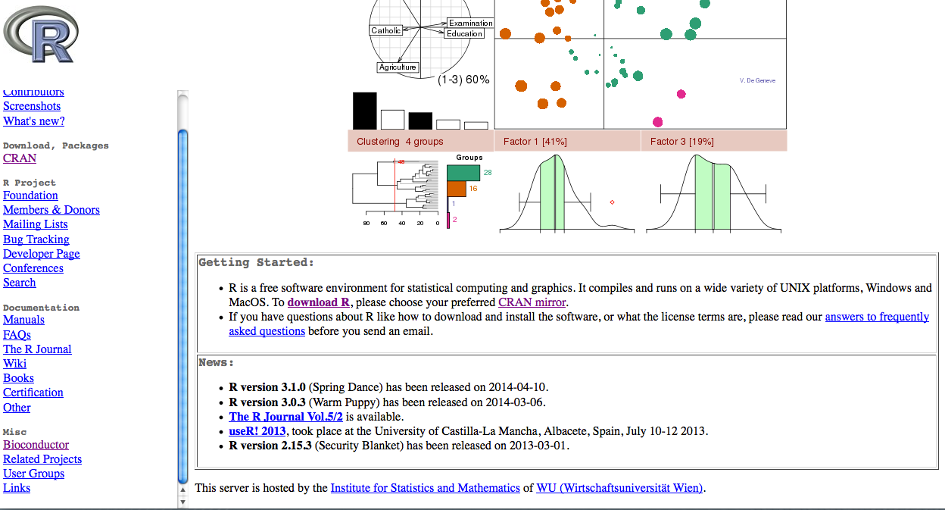
\includegraphics[width=0.8\linewidth]{Sekil1} 

}

\caption{R programının resmi internet sites}\label{fig:Sekil1}
\end{figure}

R programıyla ilgili gerekli programlara ve paketlere kolayca ulaşabilmek için dünyanın farklı yerlerinde tanımlanmış internet adresleri bulunmaktadır. İhtiyaç duyulan R programına ait paketler indirilmek istendiğinde en yakın internet adresi seçilerek dosya indirme işlemi gerçekleştirilebilir. Türkiye için Şekil \ref{fig:Sekil2}'de görüldüğü gibi Pamukkale Üniversitesi için tanımlanan \url{http://cran.pau.edu.tr} adresinden indirilebilir. Bu alan seçildiğinde artık R programıyla ilgili bütün program ve paket indirme işlemleri bu alandan gerçekleştirilebilmektedir.

\begin{figure}

{\centering 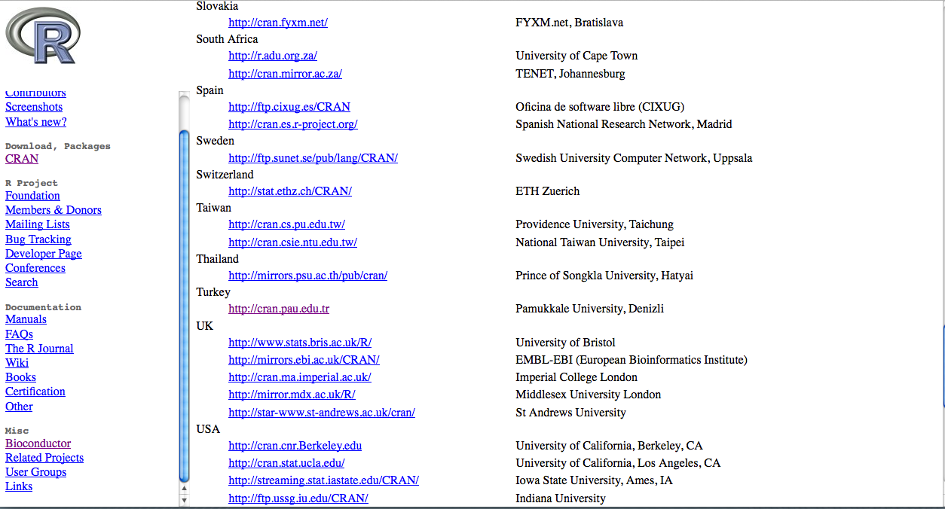
\includegraphics[width=0.8\linewidth]{Sekil2} 

}

\caption{R programı için mevcut internet siteler}\label{fig:Sekil2}
\end{figure}

Daha önce de belirtildiği gibi R programı PC-Windows, Apple Mac-OS ve Linux işletim sistemlerinde çalıştıralabilmektedir. Bu amaçla, Şekil \ref{fig:Sekil3}'de görüldüğü gibi kullandığınız işletim sistemiyle uyumlu olan R programı kolayca seçilebilmektedir. Burada PC-Windows işletim sistemi kullanıldığı kabul edilerek Download R for Windows'a tıklandığında Şekil \ref{fig:Sekil4}'de verilen internet sayfasına yönlendirilerek Windows işletim sistemiyle uyumlu farklı şekilde derlenmiş R programları indirilebilir.

\begin{figure}

{\centering 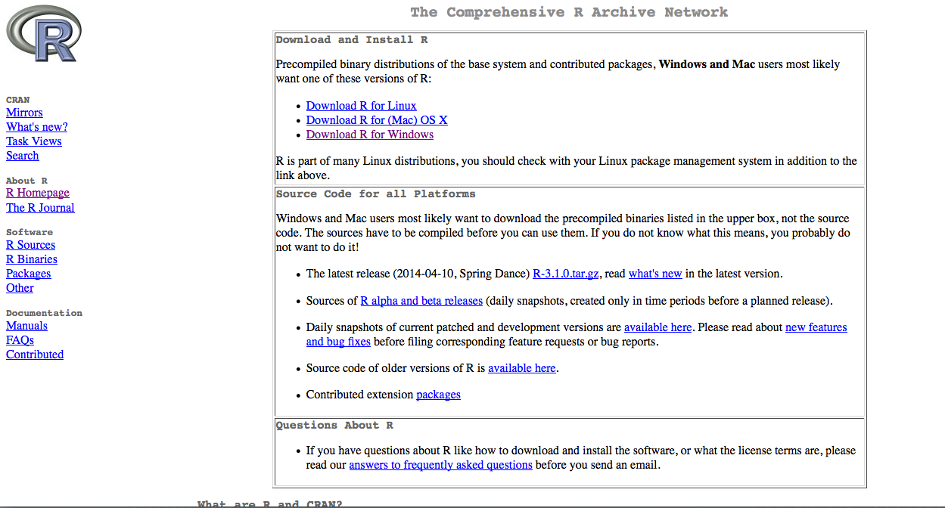
\includegraphics[width=0.8\linewidth]{Sekil3} 

}

\caption{PC-Windows, Apple Mac-OS ve Linux işletim sistemleri için R programı}\label{fig:Sekil3}
\end{figure}

Şekil \ref{fig:Sekil4}'de verilen base seçeneğine tıklandığında Şekil \ref{fig:Sekil5}'de görülen sayfaya yönlendirilerek önceden derlenmiş \textbf{Download R for Windows} dosyası indirilerek kurulum gerçekleştirilebilir (R programının Download R3.1.1 for Windows gibi en son versiyonunu belirtmektedir).

\begin{figure}

{\centering 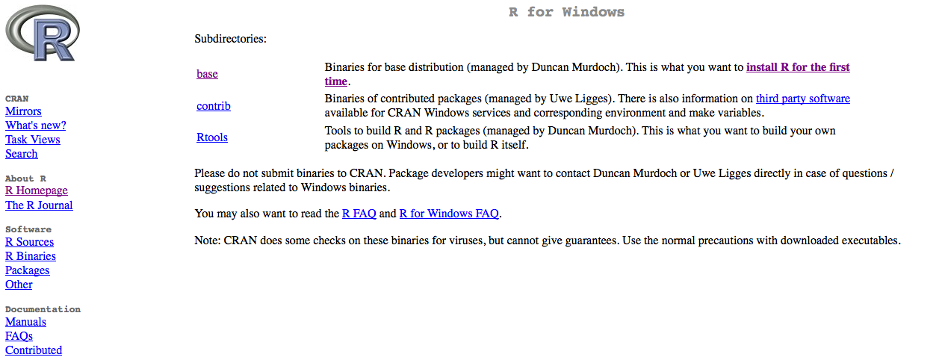
\includegraphics[width=0.8\linewidth]{Sekil4} 

}

\caption{R programının farklı şekilde derlenmiş türleri}\label{fig:Sekil4}
\end{figure}

\begin{figure}

{\centering 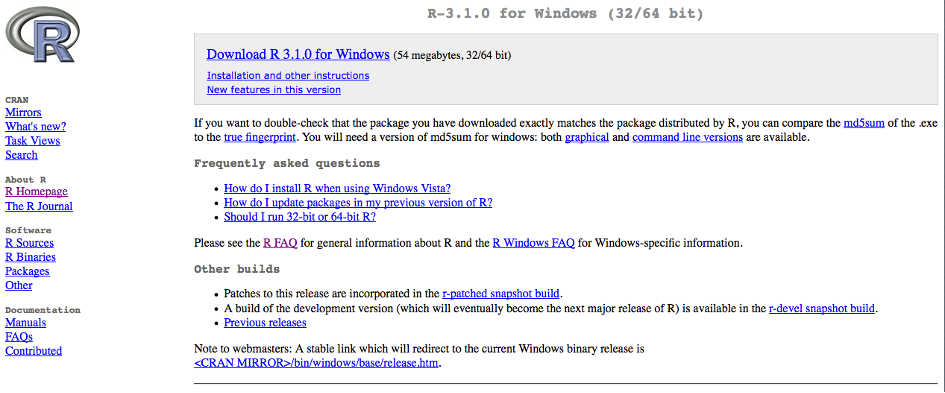
\includegraphics[width=0.8\linewidth]{Sekil5} 

}

\caption{ R programının PC-Windows işletim sistemi için kurulum dosya}\label{fig:Sekil5}
\end{figure}

\section{R Programını Başlatmak ve Kapatmak}\label{r-programux131nux131-baux15flatmak-ve-kapatmak}

R programını kullanmanın en kolay yolu, komut yazma ve sonuç alma şeklinde interaktif olarak kullanmaktır. R programı \textbf{PC-Windows} veya \textbf{Mac OS X} işletim sistemli bilgisayara kurulduktan sonra, R ikonuna tıklayarak başlatılabilir ve Şekil \ref{fig:Sekil6}'da verilen programın grafiksel kullanıcı arayüz penceresi açılır.

\begin{figure}

{\centering 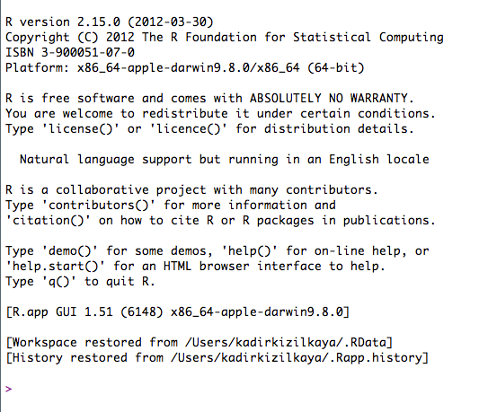
\includegraphics[width=0.8\linewidth]{Sekil6} 

}

\caption{R programının kullanıcı arayüzü (konsol)}\label{fig:Sekil6}
\end{figure}

R konsolunda yer alan açılış mesajının altında \textgreater{} ``büyüktür'' işareti yer alır. Birçok kısımda, R programı içerisindeki komutlar veya ifadeler R konsol penceresine doğrudan yazılır.

R programı başlatıldığında, Şekil \ref{fig:Sekil6}'da verilene benzer bir şekilde komut satırı belirir.

R konsolunda \texttt{\textgreater{}} durumunda yapılacak işlemle ilgili komut girildiğinde R programı işlemi gerçekleştirir ve sonucu konsol ekranına yazar.

\begin{Shaded}
\begin{Highlighting}[]
\NormalTok{y }\OtherTok{\textless{}{-}} \DecValTok{1} \SpecialCharTok{+} \DecValTok{2} 
\NormalTok{y }
\end{Highlighting}
\end{Shaded}

\begin{verbatim}
## [1] 3
\end{verbatim}

Ayrıca, R programında aşağıda verilen grafik türünde bir çıktı oluşturulacak ise bu çıktı, açılan yeni grafik penceresinde görüntülenir.

\begin{Shaded}
\begin{Highlighting}[]
\FunctionTok{plot}\NormalTok{(}\FunctionTok{rnorm}\NormalTok{(}\DecValTok{10}\NormalTok{), }\AttributeTok{ylab=}\StringTok{""}\NormalTok{, }\AttributeTok{xlab=}\StringTok{""}\NormalTok{, }\AttributeTok{cex=}\FloatTok{0.7}\NormalTok{, }\AttributeTok{cex.axis=}\FloatTok{0.7}\NormalTok{)}
\end{Highlighting}
\end{Shaded}

\begin{center}\includegraphics[width=0.8\linewidth]{R-Program_files/figure-latex/Sekil8-1} \end{center}

İşlemler için yazılan komut bir satıra sığmayacak kadar 128 karakterden uzun olduğunda veya tamamlanmadan işlem yapıldığında, komut yazma işleminin devam ettiğini belirtmek için yeni satırın başında `+' işareti görüntülenir. Bu durumda, komutun eksik olan kısmı ``+'' işaretinden sonra tamamlanarak enter tuşuna basılır ve işlem gerçekleştirilir.

\begin{Shaded}
\begin{Highlighting}[]
\NormalTok{y }\OtherTok{\textless{}{-}} \DecValTok{3}\SpecialCharTok{*} 
\SpecialCharTok{+} \DecValTok{2} 
\NormalTok{y }
\end{Highlighting}
\end{Shaded}

\begin{verbatim}
## [1] 6
\end{verbatim}

R konsol veya komut penceresinde \texttt{q()} yazarak veya pencereler doğrudan kapatılarak R programından çıkılabilir. R programından çıkış tamamlanmadan önce R oturumunda gerçekleştirilen işlemlerin kaydedilip edilmeyeceğini belirten Şekil \ldots{} deki gibi bir pencere ortaya çıkar ve bu oturumda işlemler Yes (Evet) tuşuna tıklanarak çalışma klasörü içerisine \texttt{.Rhistory} şeklinde kaydedilir. Böylece, aynı işlemlere gelecek oturumda devam edilmek istendiğinde bu \texttt{.Rhistory} dosyası kullanılarak R programı açılır ve önceki oturumda oluşturulan nesneler (değişkenler) tekrar belleğe yüklenir.

\section{Paket Kurulumu}\label{paket-kurulumu}

R programında kullanılacak bütün fonksiyonlar paketler halinde tanımlanmıştır. Gerekli fonksiyonları kullanmak için yapılması gereken fonksiyonla ilgili paketinin \texttt{install.packages()} komutu kullanılarak R programı içerisinde bilgisayara kurulmasıdır. Bu komut içerisinde her hangi bir paket ismi belirtilmeden \texttt{install.packages()} şeklinde kullanıldığında CRAN sisteminde mevcut bütün paketler listelenecektir ve paketlerden bir tanesi seçildiğinde bu paket bilgisayara indirilerek kurulacaktır. Buna karşılık, \texttt{ggplot2} gibi bir grafik paketi yüklenmek istendiğinde \texttt{install.packages(ggplot2)} şeklinde tanımlanarak gerçekleştirilebilir.

Fonksiyonla ilgili gerekli paketin bilgisayara bir kez kurulması yeterlidir. Fakat, paketi oluşturan yazarlar paketler güncellenebilmektedir. Bu yüzden, belirli aralıklarla paketlerin kurulumunun da \texttt{update.packages()} komutu kullanılarak güncellenmesi R programının daha etkili kullanımını sağlayacağından önemlidir. Bilgisayarınıza yüklü paketlerin listesi, versiyon numarası, ilişkili olduğu diğer paketler ve özellikleri \texttt{installed.packages()} komutu kullanılarak görülebilir.

\section{Paket Yükleme}\label{paket-yuxfckleme}

Herhangi bir R programında herhangi bir fonksiyonun paketi, dünyanın farklı yerlerindeki CRAN internet sitelerinden bilgisayardaki R programına ait kütüphaneye indirilebilir. R programında açılan bir oturumda bir fonksiyon kullanılmadan önce \texttt{library()} komutuyla fonksiyonla ilgili gerekli paket yüklenmelidir. Örneğin ggplot kullanılarak grafik çizdirilmek istendiğinde

\begin{Shaded}
\begin{Highlighting}[]
\FunctionTok{library}\NormalTok{(ggplot2)}
\end{Highlighting}
\end{Shaded}

şeklinde yüklenmelidir. Gerekli paketin açılan oturumda bir kere yüklenmesi yeterlidir. Fakat, oturum kapatıldığında ve açılan yeni oturumda bu paket tekrar kullanılmak istendiğinde yine \texttt{library()} komutuyla tekrar yüklenmelidir. Çok sık kullanılan fonksiyonlara ait paketler bilgisayarın başlatma komutlarına eklenerek doğrudan yüklenmeleri de sağlanabilir.

\section{Paketler}\label{paketler}

R programı matematiksel, istatistiksel ve grafiksel işlemlerle ilgili paketleri içermektedir. Bu paketler, konularla ilgili fonksiyonların, verilerin ve derlenmiş kodların bir bütün halinde R programında sunulması olarak düşünülebilir. R programındaki paketlere ait kütüphanenin bilgisayarın neresinde oluşturulduğu \texttt{.libPaths()} komutuyla öğrenilebilir. Ayrıca \texttt{library()} komutuyla hangi paketlerin yüklü olduğu da kolayca belirlenebilir.

\begin{Shaded}
\begin{Highlighting}[]
\FunctionTok{.libPaths}\NormalTok{()}
\end{Highlighting}
\end{Shaded}

\begin{verbatim}
## [1] "/Library/Frameworks/R.framework/Versions/4.2/Resources/library"
\end{verbatim}

R programında bir oturum başlatıldığında \texttt{base}, \texttt{datasets}, \texttt{utils}, \texttt{grDevices}, \texttt{graphics}, \texttt{stats} ve \texttt{methods} paketleri standart olarak doğrudan yüklenmektedir. Ayrıca, ihtiyaç duyulan paketler de yukarı da açıklandığı şekilde yüklenebilir. Buna ek olarak, hangi paketlerin yüklendiği ve kullanım için hazır olup olmadığı \texttt{search()} komutu kullanılarak belirlenebilir.

\begin{Shaded}
\begin{Highlighting}[]
\FunctionTok{search}\NormalTok{()}
\end{Highlighting}
\end{Shaded}

\begin{verbatim}
##  [1] ".GlobalEnv"        "package:ggplot2"   "package:stats"    
##  [4] "package:graphics"  "package:grDevices" "package:utils"    
##  [7] "package:datasets"  "package:methods"   "Autoloads"        
## [10] "package:base"
\end{verbatim}

\section{Betik (Script) Oluşturma}\label{betik-script-oluux15fturma}

Betik (Script), bilgisayar programlama (yazılım) alanında kullanıldığı anlamıyla; herhangi bir programlama (yazılım) dilinde oluşturulmuş kodları (kod bloğunu) içeren dosyayı ifade eder. Genel anlamda, programlama (yazılım) dilinde oluşturulmuş kodları çalıştırmak gerektiğinde tekrar tekrar yazmak yerine; bu kodları içeren betik (script) dosyası yüklenerek kodlar kolayca çalıştırılabilir.

Betik dosyası Şekil \ref{fig:Sekil13}'de \texttt{File} (Dosya)'dan \texttt{New\ Document} seçilir.

\begin{figure}

{\centering 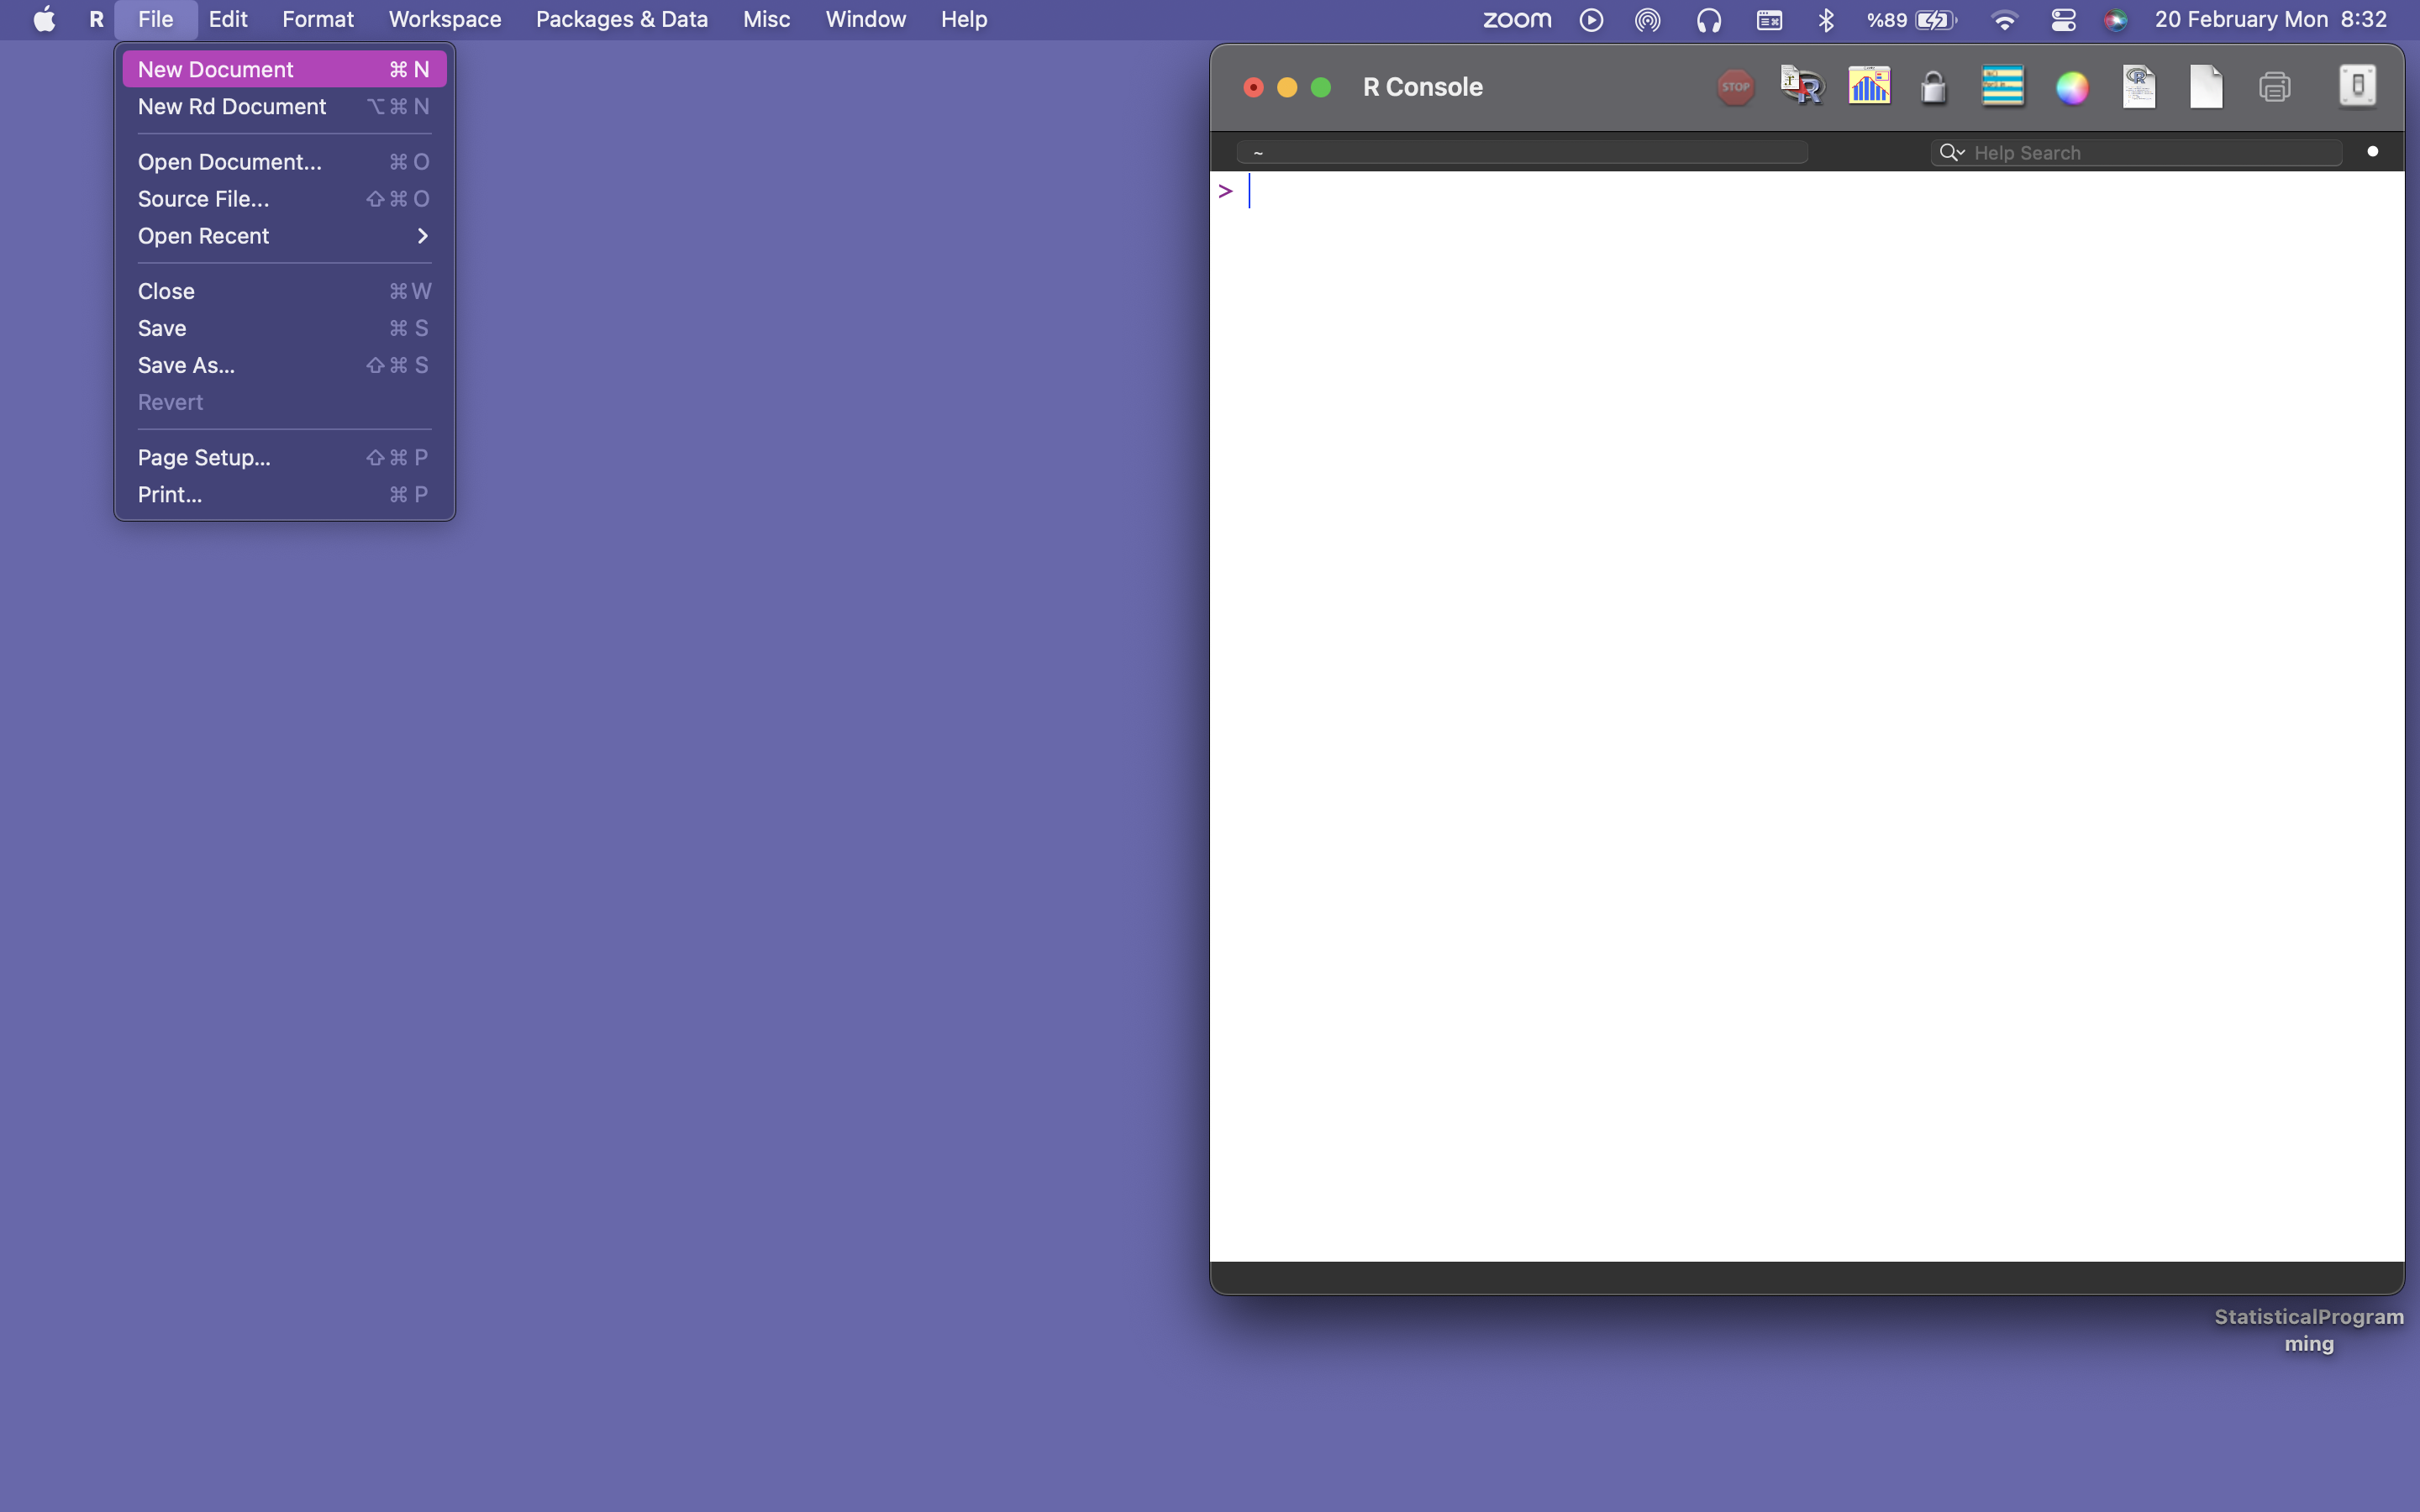
\includegraphics[width=0.8\linewidth]{Script1} 

}

\caption{Betik dosyası oluşturma}\label{fig:Sekil13}
\end{figure}

Şekil \ref{fig:Sekil14} görüldüğü gibi boş yeni bir betik dosyası açılır.

\begin{figure}

{\centering 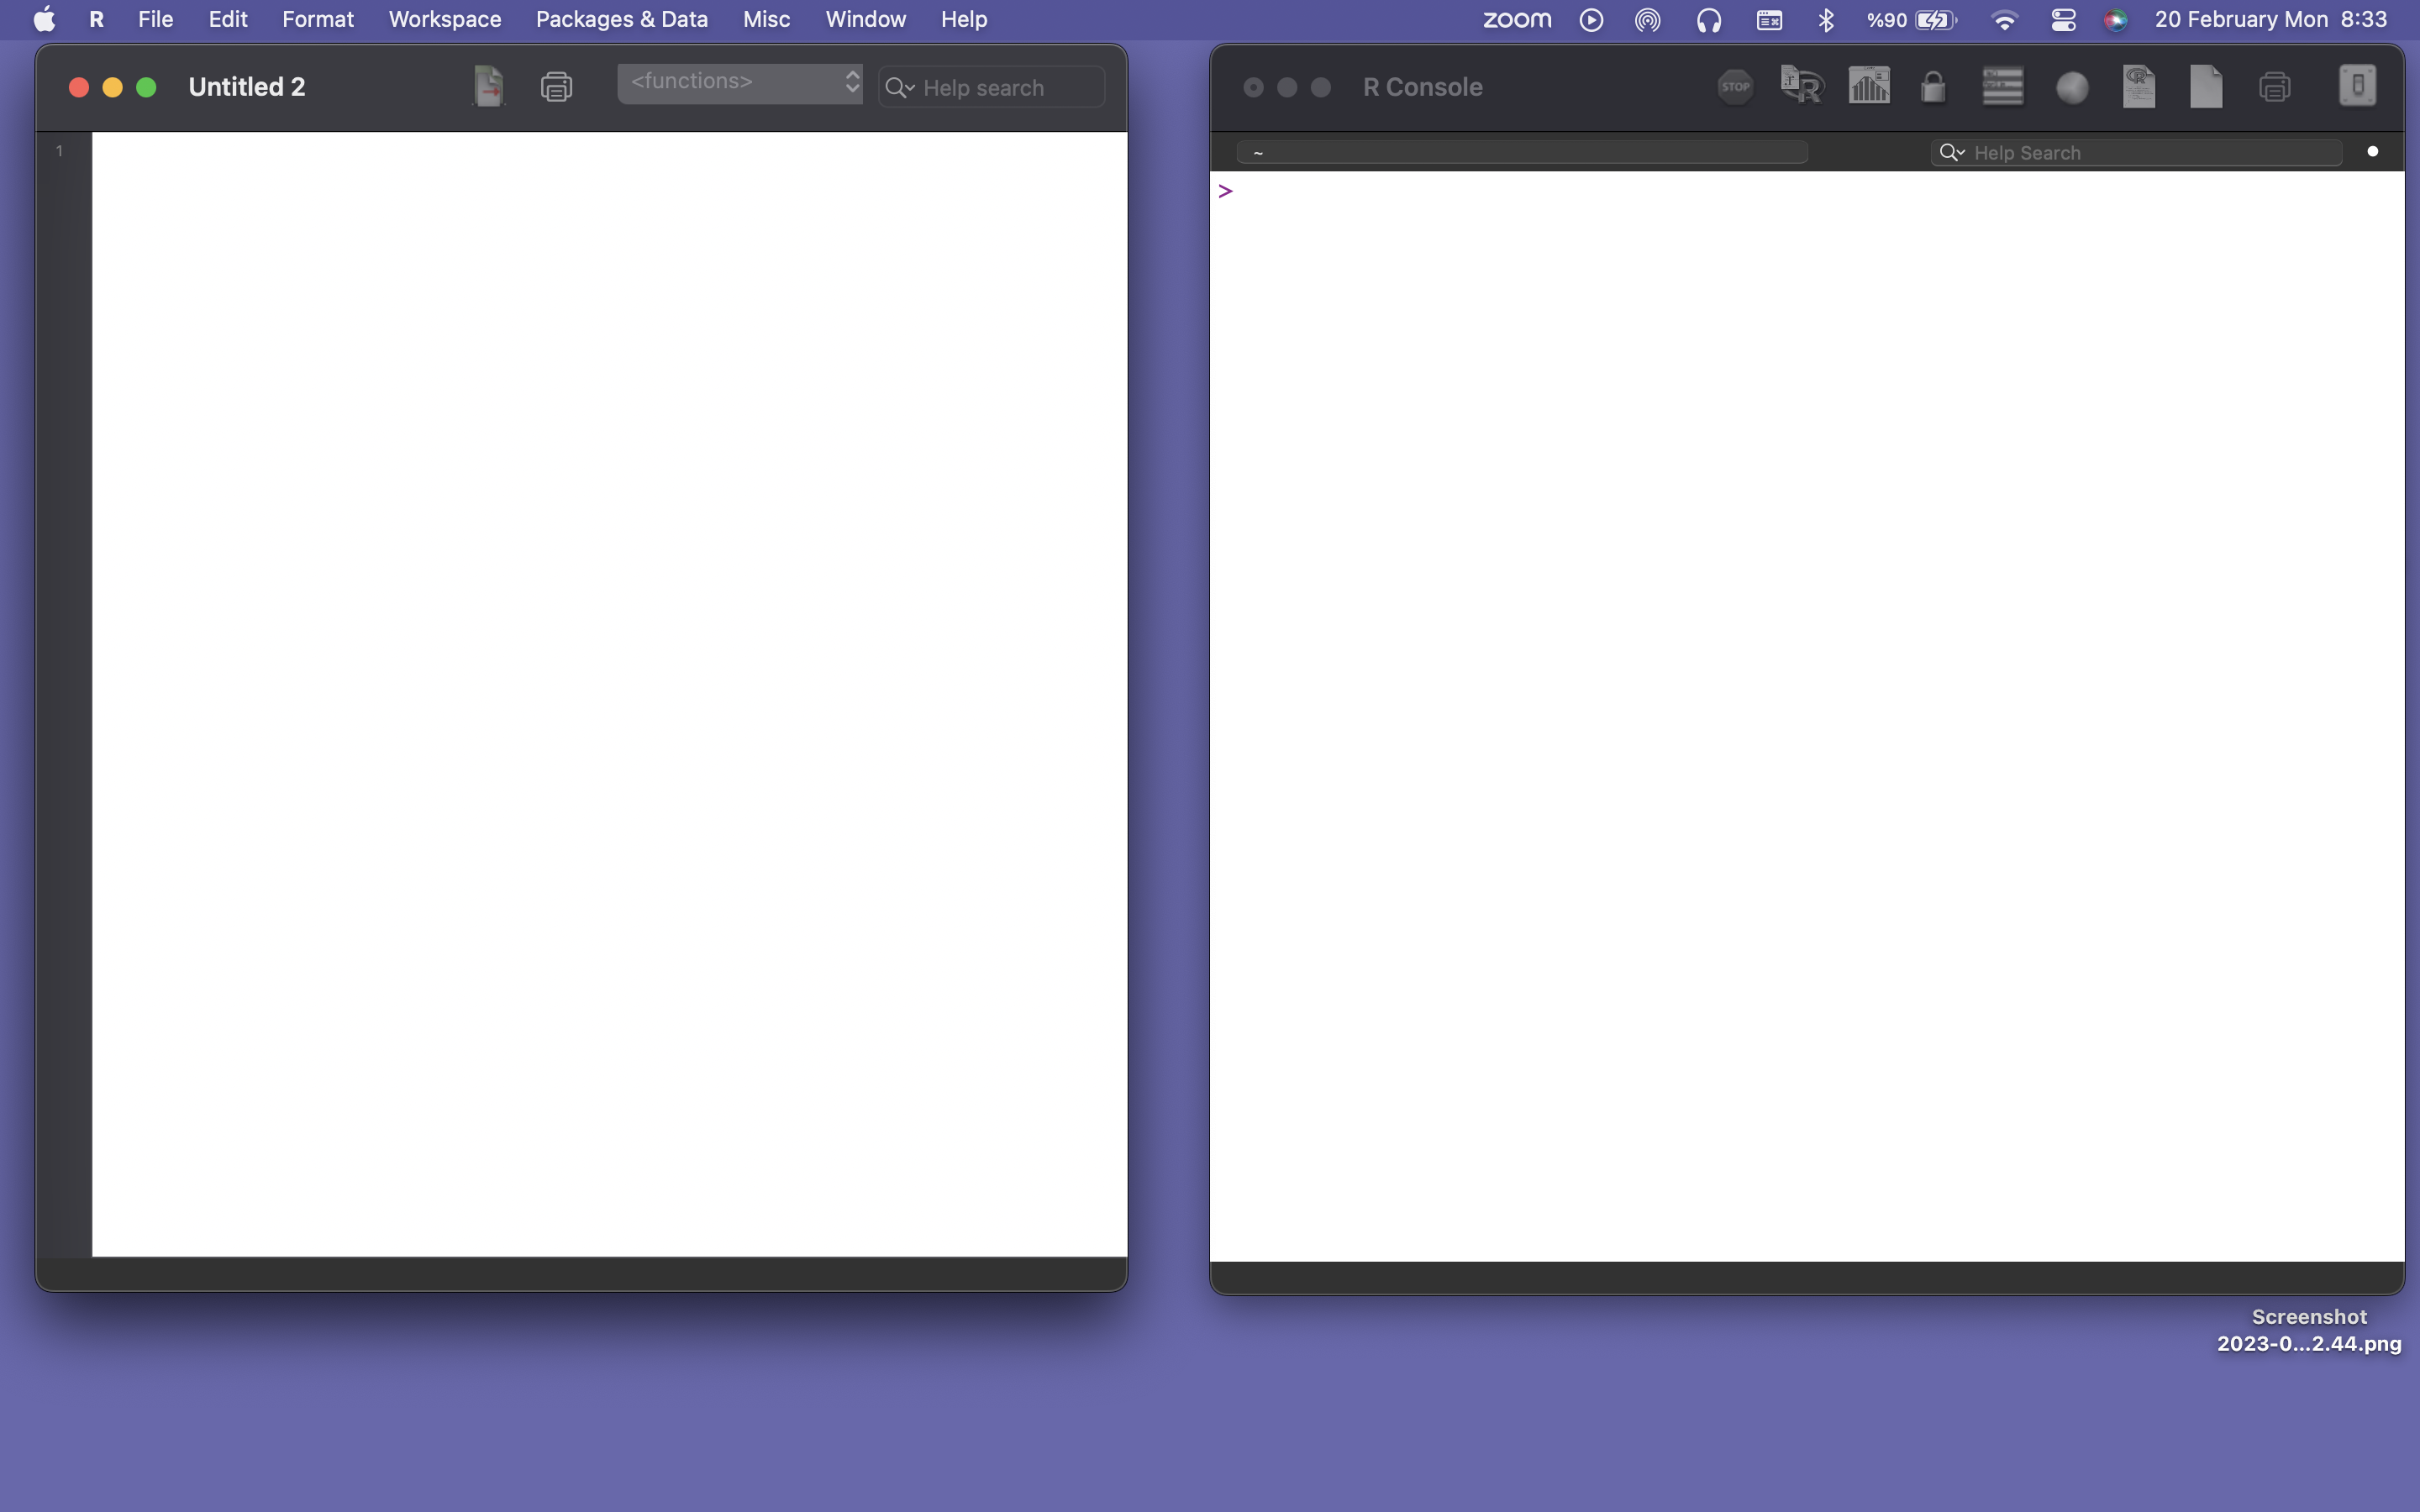
\includegraphics[width=0.8\linewidth]{Script2} 

}

\caption{Yeni Betik dosyası açıldı}\label{fig:Sekil14}
\end{figure}

Açılan betik dosyası Şekil \ref{fig:Sekil15} görüldüğü gibi dosyanın uzantısı \texttt{.R} olacak şekilde herhangi bir isimle kaydedilir.

\begin{figure}

{\centering 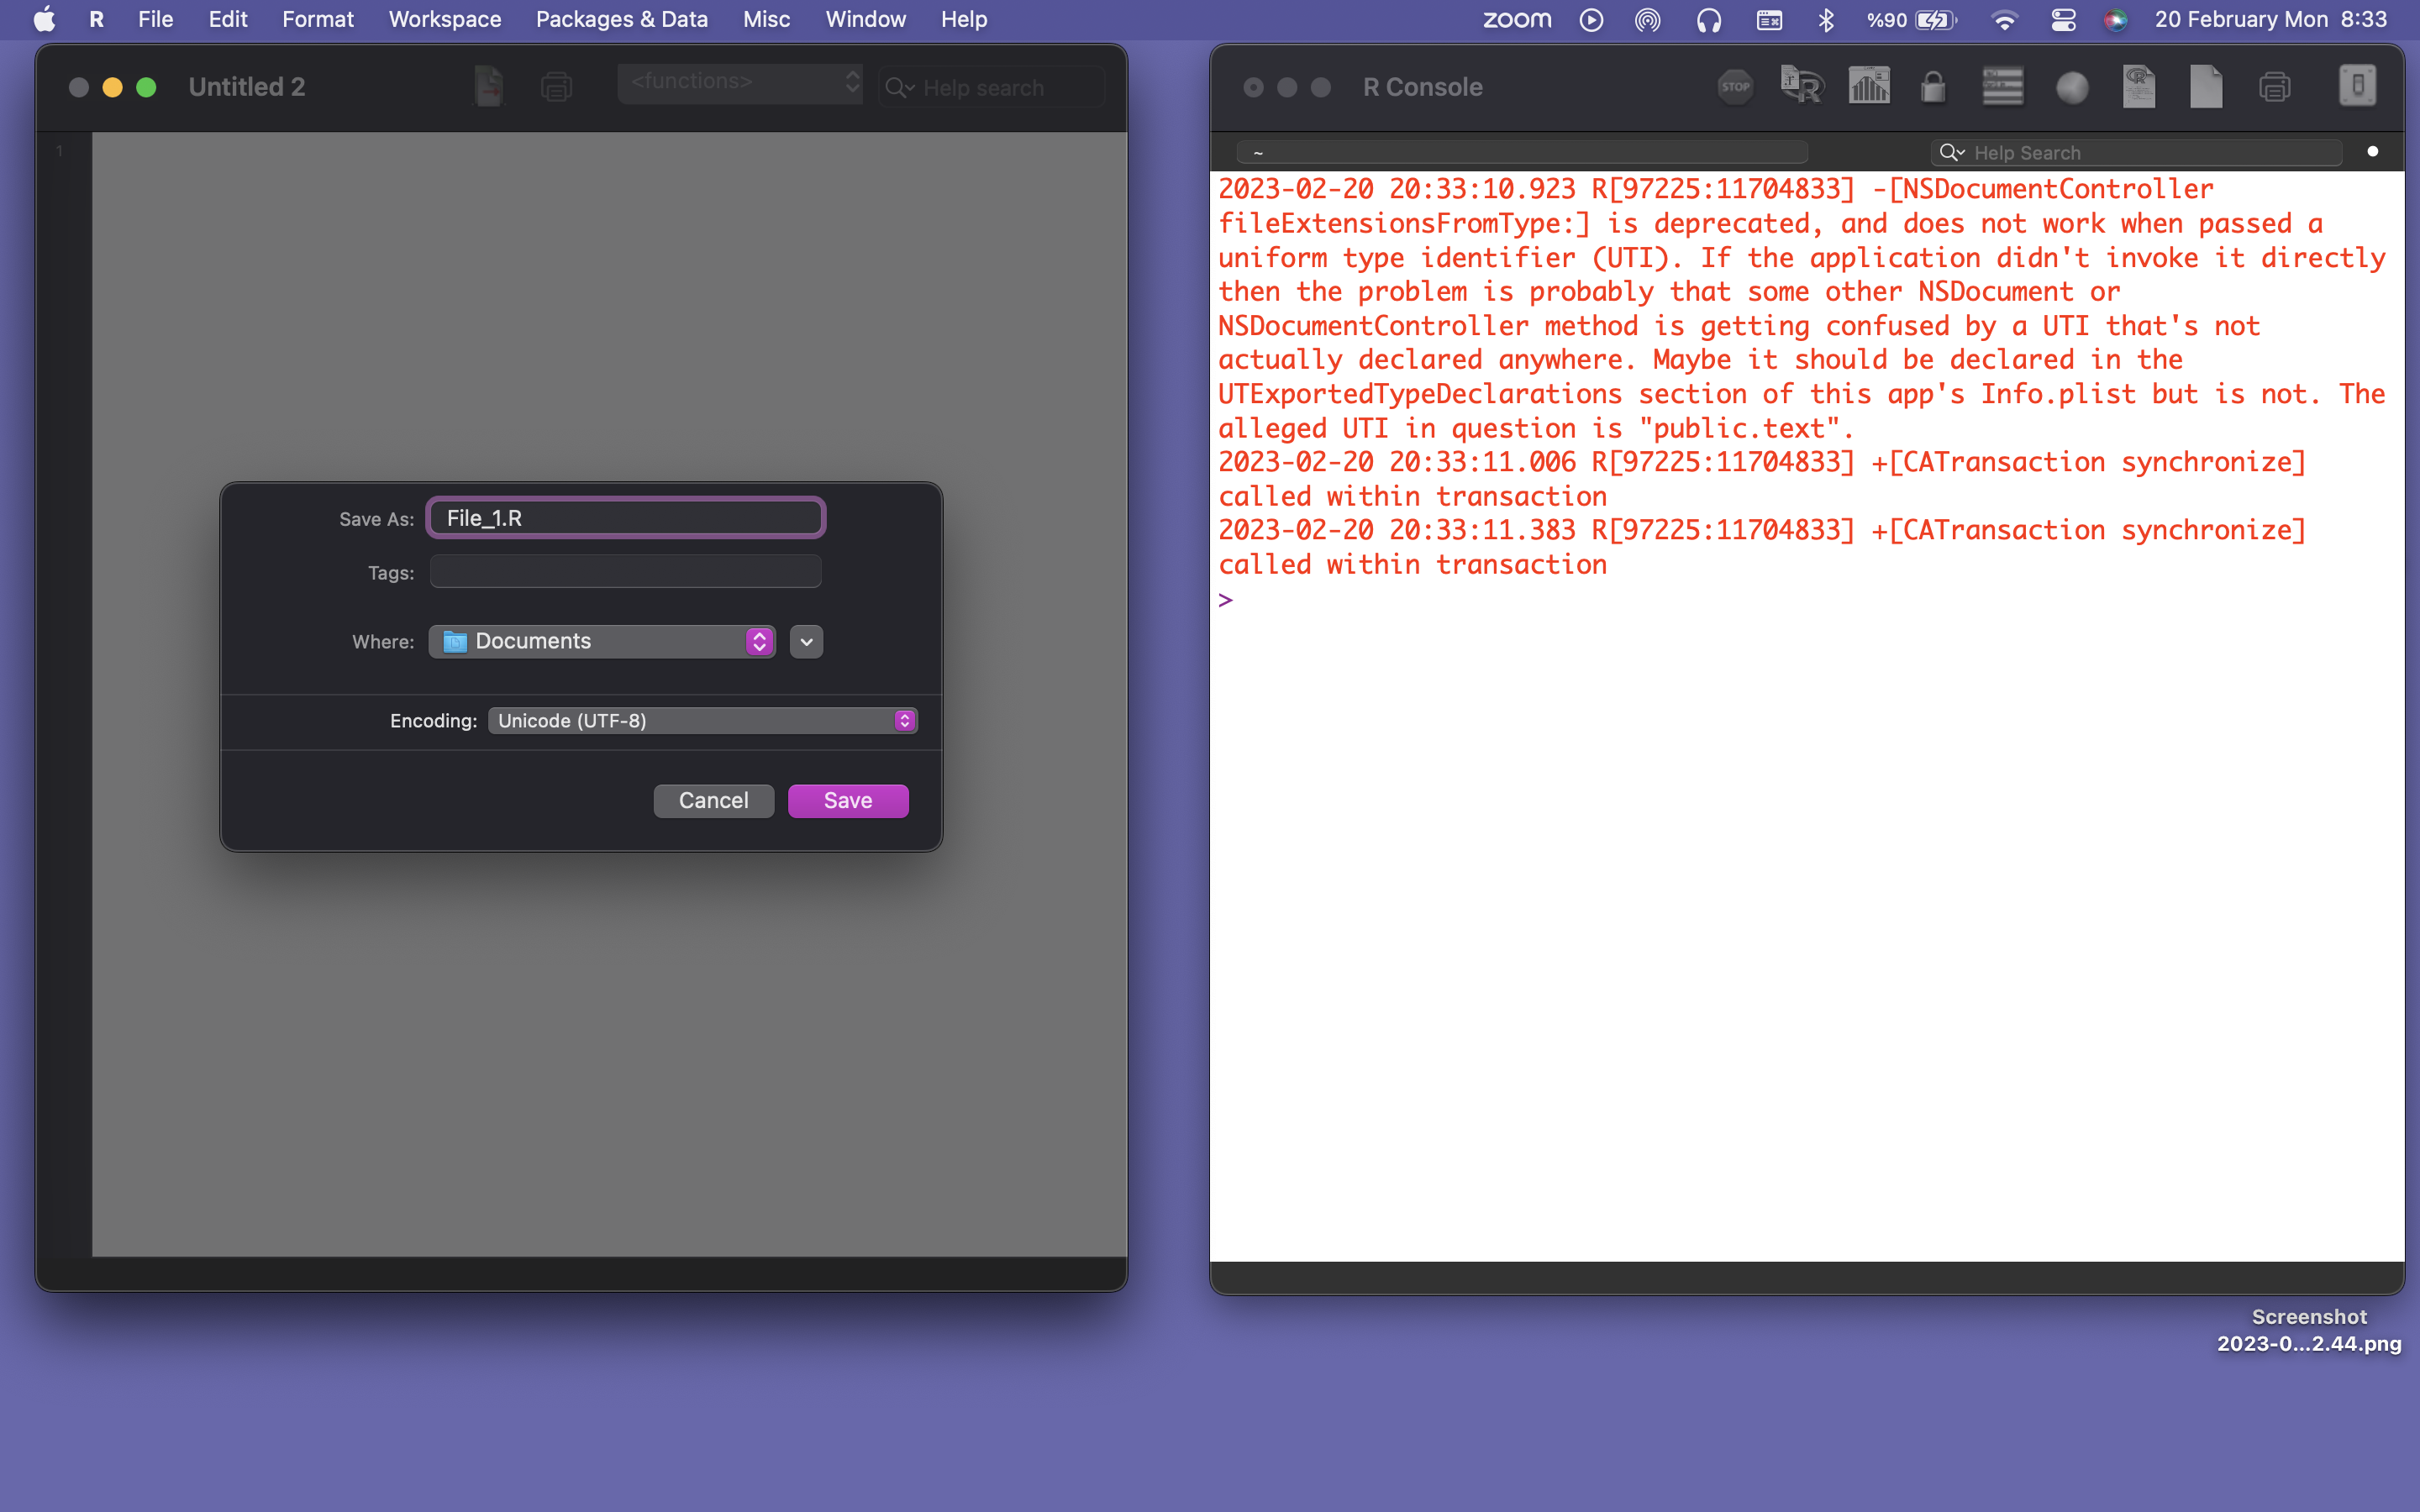
\includegraphics[width=0.8\linewidth]{Script3} 

}

\caption{Betik dosyası uznatısı .R olacak şekilde herhangi bir isimle kaydedilir}\label{fig:Sekil15}
\end{figure}

Açılan betik dosyasına Şekil \ref{fig:Sekil16} görüldüğü gibi kodlar yazılır ve \texttt{Edit} içerisinde yer alan \texttt{Execute} seçilerek kodlar çalıştırılır.

\begin{figure}

{\centering 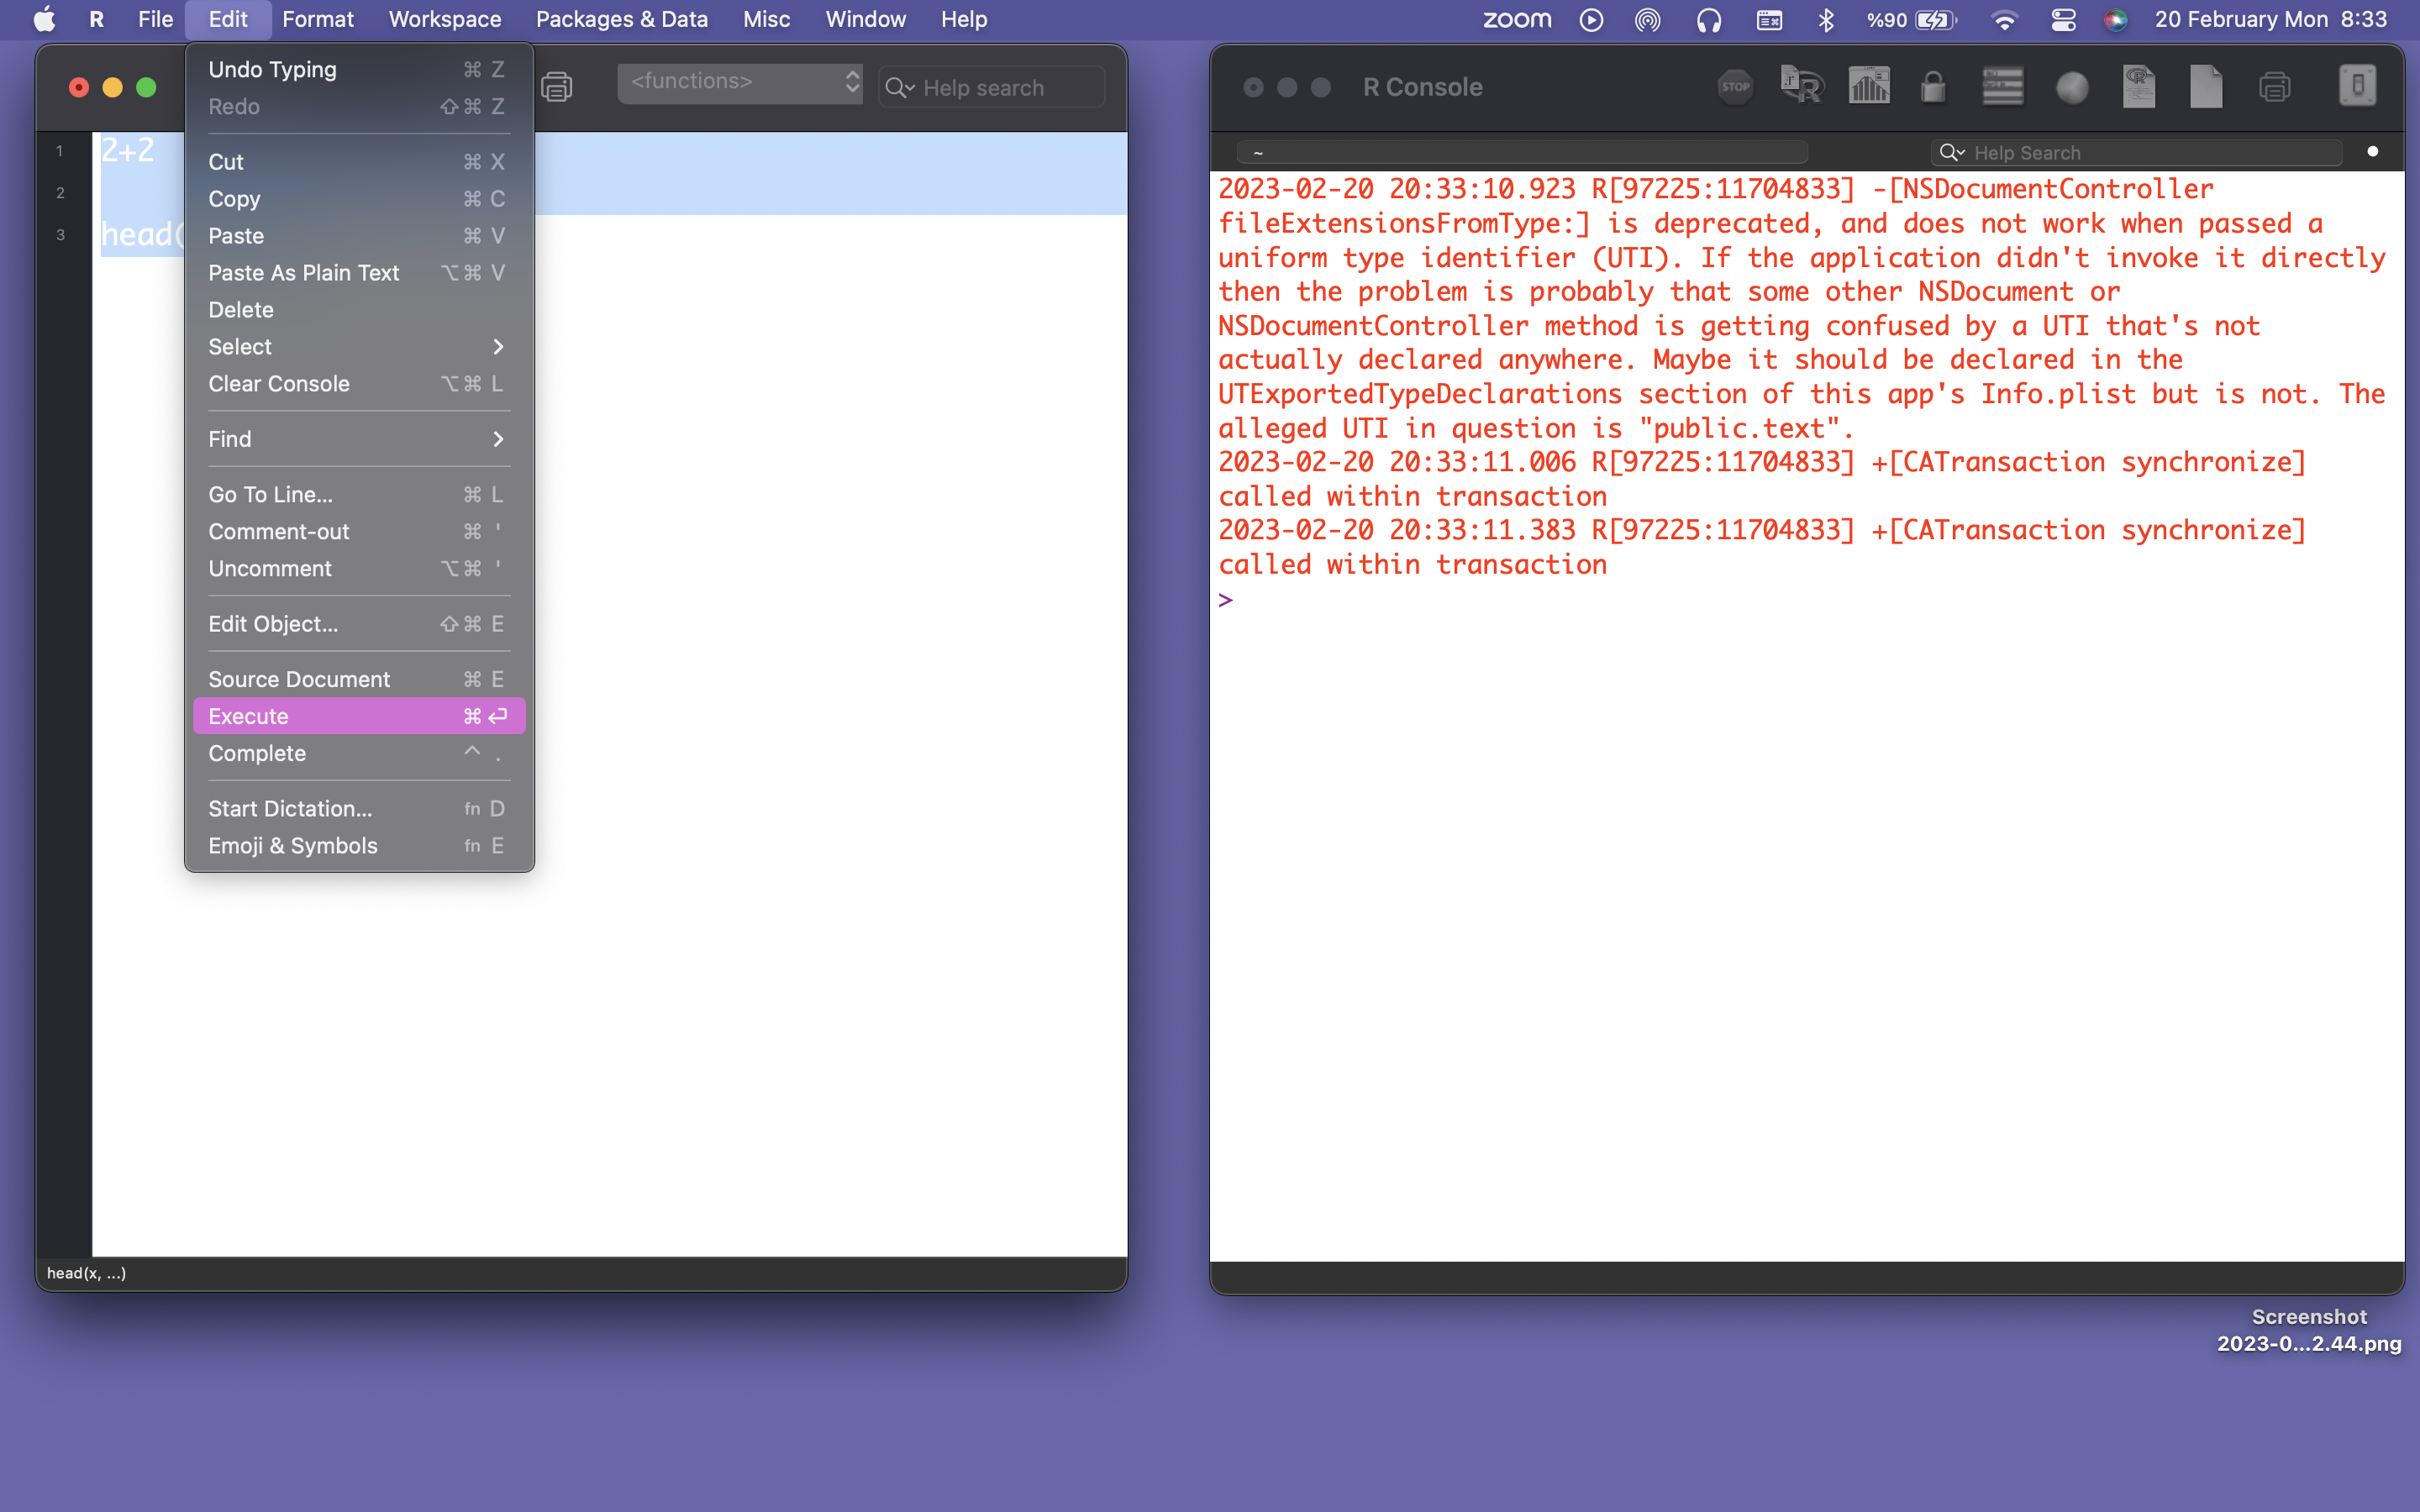
\includegraphics[width=0.8\linewidth]{Script4} 

}

\caption{Betik dosyasına kodların yazılması ve çalıştırılması}\label{fig:Sekil16}
\end{figure}

Betik dosyasındaki kodların çalıştırılmasına ait sonuçlar Şekil \ref{fig:Sekil17} görüldüğü \texttt{Console} penceresinde görüntülenir.

\begin{figure}

{\centering 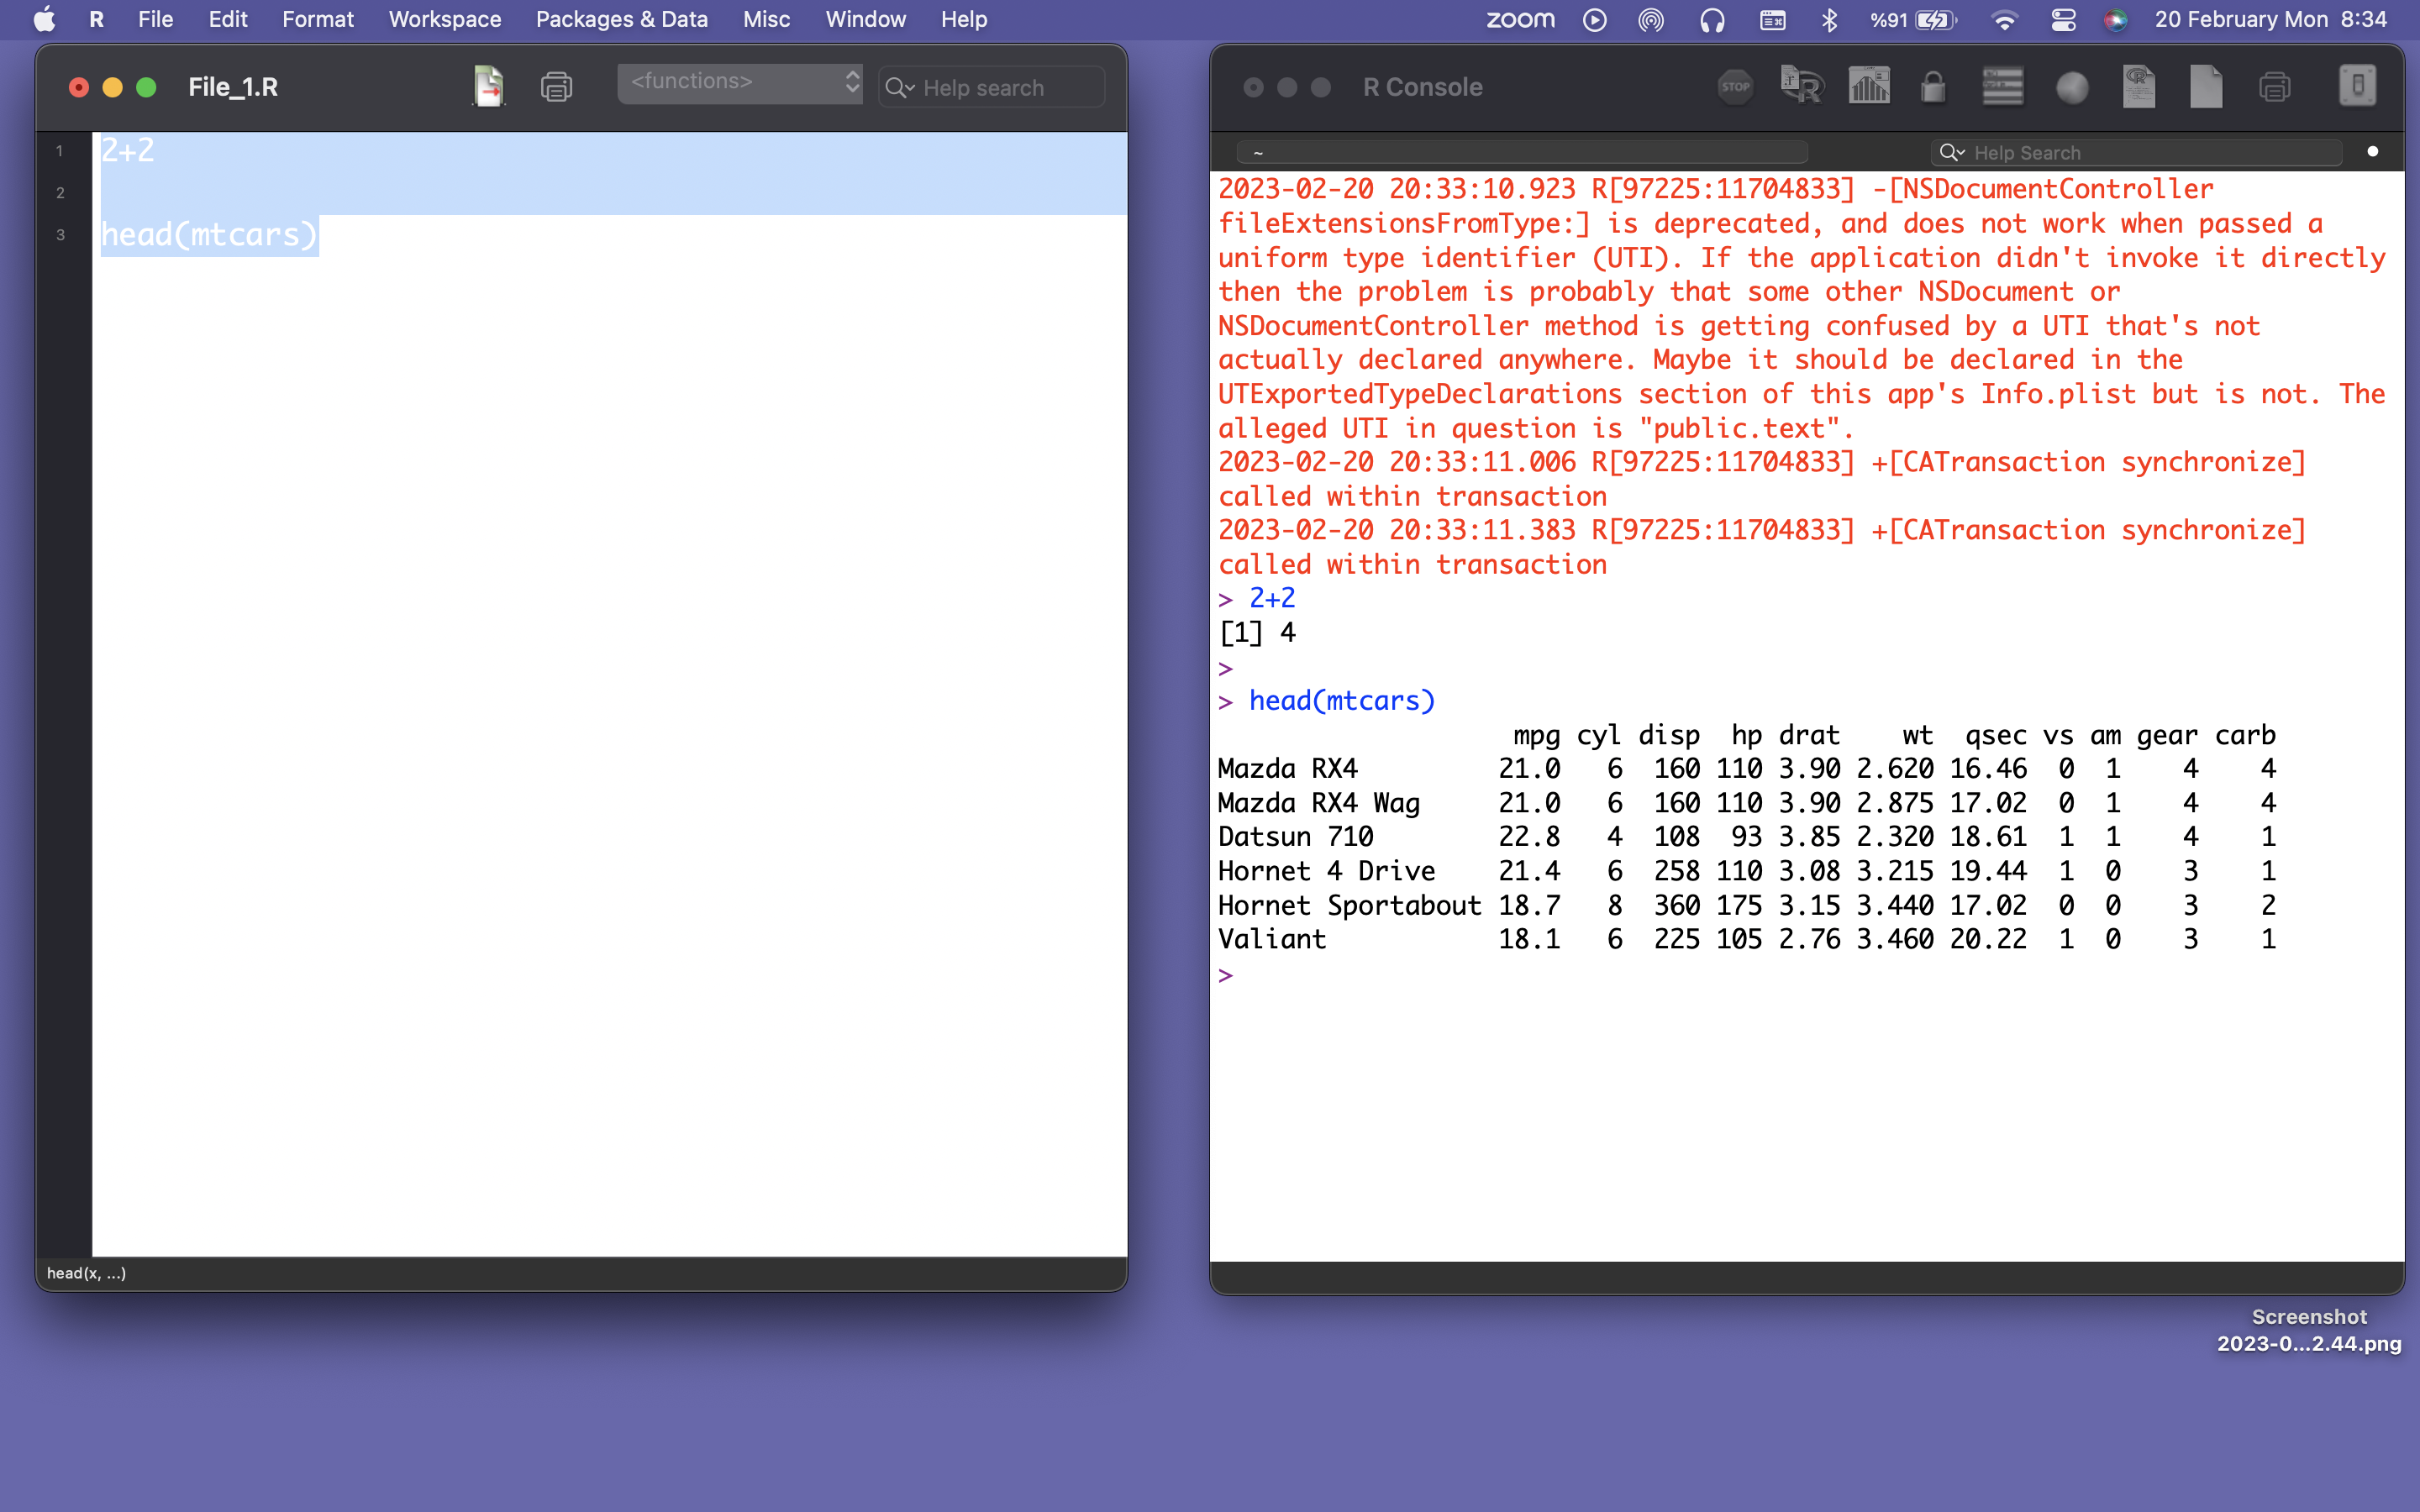
\includegraphics[width=0.8\linewidth]{Script5} 

}

\caption{Betik dosyasının çalıştırılması sonucu elde edilen sonuçlar}\label{fig:Sekil17}
\end{figure}

\chapter{Genel Kurallar ve Komutlar}\label{genel-kurallar-ve-komutlar}

\section{R Programında Geçerli Değişken İsimleri}\label{r-programux131nda-geuxe7erli-deux11fiux15fken-isimleri}

R programında değişken isimleri harflerin, rakamların ve noktaların `.' birleşimiyle oluşturulabilir. Yalnız,

\begin{itemize}
\tightlist
\item
  değişken isimleri için R programında tanımlı `c' veya `mean' gibi fonksiyon isimlerinin kullanılmamasına,
\item
  değişken isimlerinde Türkçe karakter Ç, Ğ, İ, Ö, Ş, Ü ve ç, ğ, ı, ö, ş, ü kullanılmamasına,
\item
  değişken isimlerinin rakam (0, 1, 2, 3, 4, 5, 6, 7, 8, 9) ile başlamamasına,
  dikkat edilmelidir. Ayrıca, R programında büyük ve küçük harf farklılığı olup, A ve a şeklinde kullanılan değişkenler aşağıda görüldüğü gibi birbirinden farklıdır.
\end{itemize}

\begin{Shaded}
\begin{Highlighting}[]
\NormalTok{A }\OtherTok{\textless{}{-}} \DecValTok{10}\SpecialCharTok{*}\DecValTok{2} 
\NormalTok{A}
\end{Highlighting}
\end{Shaded}

\begin{verbatim}
## [1] 20
\end{verbatim}

\begin{Shaded}
\begin{Highlighting}[]
\NormalTok{a }\OtherTok{\textless{}{-}} \DecValTok{15}\SpecialCharTok{/}\DecValTok{3} 
\NormalTok{a }
\end{Highlighting}
\end{Shaded}

\begin{verbatim}
## [1] 5
\end{verbatim}

\section{Boşluk}\label{boux15fluk}

R programlama dili, aşağıda görüldüğü gibi işlemleri gerçekleştirirken değişken isimleri ve operatörler (işlet) arasındaki boşlukları dikkate almaz.

\begin{Shaded}
\begin{Highlighting}[]
\NormalTok{x }\OtherTok{\textless{}{-}} \DecValTok{1} \SpecialCharTok{+} \DecValTok{3} 
\NormalTok{x }
\end{Highlighting}
\end{Shaded}

\begin{verbatim}
## [1] 4
\end{verbatim}

Buna karşılık, değişkene değer atama operatöründe (\textless-), \textless{} ile - arasında boşluk verilmemelidir. Boşluk verildiğinde aşağıdaki gibi farklı bir sonuç elde edilebilir.

\begin{Shaded}
\begin{Highlighting}[]
\NormalTok{x }\SpecialCharTok{\textless{}} \SpecialCharTok{{-}}\DecValTok{1} \SpecialCharTok{+} \DecValTok{3}
\end{Highlighting}
\end{Shaded}

\begin{verbatim}
## [1] FALSE
\end{verbatim}

Aşağıda verilen örneklerde açıkça görüldüğü gibi yazı karakterleri arasında boşluk kullanıldığında da dikkatli olunmalıdır.

\begin{Shaded}
\begin{Highlighting}[]
\NormalTok{y }\OtherTok{\textless{}{-}} \StringTok{"A B C D"} 
\NormalTok{y }
\end{Highlighting}
\end{Shaded}

\begin{verbatim}
## [1] "A B C D"
\end{verbatim}

\begin{Shaded}
\begin{Highlighting}[]
\NormalTok{z }\OtherTok{\textless{}{-}} \StringTok{"A   B   C   D"} 
\NormalTok{z }
\end{Highlighting}
\end{Shaded}

\begin{verbatim}
## [1] "A   B   C   D"
\end{verbatim}

\section{\texorpdfstring{Çalışma Dizininin Belirlenmesi \texttt{getwd()}}{Çalışma Dizininin Belirlenmesi getwd()}}\label{uxe7alux131ux15fma-dizininin-belirlenmesi-getwd}

R programında \texttt{getwd()} fonksiyonunun açılımı get working directory'dir ve çalışma dizini veya içerisinde çalışılan dizin aşağıdaki örnekte olduğu gibi \texttt{getwd()} fonksiyonu yazılarak belirlenebilir. Çalışma dizini aynı zamanda R programı araç çubuğunda Misc menüsü içerisinde Get Working Directory seçilerek de belirlenebilir.

\begin{Shaded}
\begin{Highlighting}[]
\FunctionTok{getwd}\NormalTok{()}
\end{Highlighting}
\end{Shaded}

\begin{verbatim}
## [1] "/Users/merve/Documents/R-Kitap"
\end{verbatim}

\section{\texorpdfstring{Çalışma Dizininin Değiştirilmesi \texttt{setwd()}}{Çalışma Dizininin Değiştirilmesi setwd()}}\label{uxe7alux131ux15fma-dizininin-deux11fiux15ftirilmesi-setwd}

R programında \texttt{setwd()} fonksiyonunun açılımı set working directory'dir.Değiştirilmek istenen dizin aşağıdaki örnekte olduğu gibi \texttt{setwd()} fonksiyonunda `` '' içerisinde yazılarak değiştirilebilir ve tekrar \texttt{getwd()} fonksiyonu kullanılarak içerisinde bulunan dizin belirlenebilir. R programında dizin değişikliği aynı zamanda R programı araç çubuğunda Misc menüsü içerisinde Change Working Directory seçilerek de değiştirilebilir.

\begin{Shaded}
\begin{Highlighting}[]
\FunctionTok{setwd}\NormalTok{(}\StringTok{"/Users/merve/Documents/R{-}Kitap"}\NormalTok{)}
\FunctionTok{getwd}\NormalTok{()}
\end{Highlighting}
\end{Shaded}

\begin{verbatim}
## [1] "/Users/merve/Documents/R-Kitap"
\end{verbatim}

\section{\texorpdfstring{Çalışma Dizininde Dizin ve Dosyaların Listelenmesi \texttt{dir()} veya \texttt{list.files()}}{Çalışma Dizininde Dizin ve Dosyaların Listelenmesi dir() veya list.files()}}\label{uxe7alux131ux15fma-dizininde-dizin-ve-dosyalarux131n-listelenmesi-dir-veya-list.files}

Çalışılan dizinde bulunan dizin ve dosyaların listesi konsol da \texttt{dir()} veya \texttt{list.files()} fonksiyonu yazılarak listelenebilir.

\begin{Shaded}
\begin{Highlighting}[]
\FunctionTok{list.files}\NormalTok{()}
\end{Highlighting}
\end{Shaded}

\begin{verbatim}
##  [1] "_book"                 "_bookdown_files"       "_bookdown.yml"        
##  [4] "_output.yml"           "01-RKurulum.Rmd"       "02-GenelKural.Rmd"    
##  [7] "03-VeriYapi.Rmd"       "04-Matrisler.Rmd"      "06-VektorFonk.Rmd"    
## [10] "B3_Sekil7.png"         "book.bib"              "data_tab.txt"         
## [13] "data_virgul.csv"       "data.csv"              "data.xlsx"            
## [16] "index.Rmd"             "ornek"                 "packages.bib"         
## [19] "preamble.tex"          "R Program.Rmd"         "R-Kitap.Rproj"        
## [22] "R-Program_files"       "R-Program.Rmd"         "README.md"            
## [25] "Rlogo.png"             "RRR_bookdown copy.yml" "Script1.png"          
## [28] "Script2.png"           "Script3.png"           "Script4.png"          
## [31] "Script5.png"           "Sekil1.png"            "Sekil2.png"           
## [34] "Sekil3.png"            "Sekil4.png"            "Sekil5.png"           
## [37] "Sekil6.png"            "style.css"             "Uygulama"             
## [40] "Uygulama1.R"
\end{verbatim}

veya

\begin{Shaded}
\begin{Highlighting}[]
\FunctionTok{dir}\NormalTok{()}
\end{Highlighting}
\end{Shaded}

\begin{verbatim}
##  [1] "_book"                 "_bookdown_files"       "_bookdown.yml"        
##  [4] "_output.yml"           "01-RKurulum.Rmd"       "02-GenelKural.Rmd"    
##  [7] "03-VeriYapi.Rmd"       "04-Matrisler.Rmd"      "06-VektorFonk.Rmd"    
## [10] "B3_Sekil7.png"         "book.bib"              "data_tab.txt"         
## [13] "data_virgul.csv"       "data.csv"              "data.xlsx"            
## [16] "index.Rmd"             "ornek"                 "packages.bib"         
## [19] "preamble.tex"          "R Program.Rmd"         "R-Kitap.Rproj"        
## [22] "R-Program_files"       "R-Program.Rmd"         "README.md"            
## [25] "Rlogo.png"             "RRR_bookdown copy.yml" "Script1.png"          
## [28] "Script2.png"           "Script3.png"           "Script4.png"          
## [31] "Script5.png"           "Sekil1.png"            "Sekil2.png"           
## [34] "Sekil3.png"            "Sekil4.png"            "Sekil5.png"           
## [37] "Sekil6.png"            "style.css"             "Uygulama"             
## [40] "Uygulama1.R"
\end{verbatim}

\section{\texorpdfstring{Çalışma Dizininde Dizin Oluşturma \texttt{dir.create()}}{Çalışma Dizininde Dizin Oluşturma dir.create()}}\label{uxe7alux131ux15fma-dizininde-dizin-oluux15fturma-dir.create}

Çalışma dizini içerisinde dizin oluşturmak için \texttt{dir.create()} fonksiyonu kullanılır. Aşağıdaki örnekte olduğu gibi ``/kadir/Documents'' dizini içerisinde ``ornek'' dizini \texttt{dir.create(“ornek”)} şeklinde oluşturulabilir.

\begin{Shaded}
\begin{Highlighting}[]
\FunctionTok{list.files}\NormalTok{()}
\end{Highlighting}
\end{Shaded}

\begin{verbatim}
##  [1] "_book"                 "_bookdown_files"       "_bookdown.yml"        
##  [4] "_output.yml"           "01-RKurulum.Rmd"       "02-GenelKural.Rmd"    
##  [7] "03-VeriYapi.Rmd"       "04-Matrisler.Rmd"      "06-VektorFonk.Rmd"    
## [10] "B3_Sekil7.png"         "book.bib"              "data_tab.txt"         
## [13] "data_virgul.csv"       "data.csv"              "data.xlsx"            
## [16] "index.Rmd"             "ornek"                 "packages.bib"         
## [19] "preamble.tex"          "R Program.Rmd"         "R-Kitap.Rproj"        
## [22] "R-Program_files"       "R-Program.Rmd"         "README.md"            
## [25] "Rlogo.png"             "RRR_bookdown copy.yml" "Script1.png"          
## [28] "Script2.png"           "Script3.png"           "Script4.png"          
## [31] "Script5.png"           "Sekil1.png"            "Sekil2.png"           
## [34] "Sekil3.png"            "Sekil4.png"            "Sekil5.png"           
## [37] "Sekil6.png"            "style.css"             "Uygulama"             
## [40] "Uygulama1.R"
\end{verbatim}

\begin{Shaded}
\begin{Highlighting}[]
\FunctionTok{dir.create}\NormalTok{(}\StringTok{"ornek"}\NormalTok{)}
\end{Highlighting}
\end{Shaded}

\begin{verbatim}
## Warning in dir.create("ornek"): 'ornek' already exists
\end{verbatim}

\begin{Shaded}
\begin{Highlighting}[]
\FunctionTok{list.files}\NormalTok{()}
\end{Highlighting}
\end{Shaded}

\begin{verbatim}
##  [1] "_book"                 "_bookdown_files"       "_bookdown.yml"        
##  [4] "_output.yml"           "01-RKurulum.Rmd"       "02-GenelKural.Rmd"    
##  [7] "03-VeriYapi.Rmd"       "04-Matrisler.Rmd"      "06-VektorFonk.Rmd"    
## [10] "B3_Sekil7.png"         "book.bib"              "data_tab.txt"         
## [13] "data_virgul.csv"       "data.csv"              "data.xlsx"            
## [16] "index.Rmd"             "ornek"                 "packages.bib"         
## [19] "preamble.tex"          "R Program.Rmd"         "R-Kitap.Rproj"        
## [22] "R-Program_files"       "R-Program.Rmd"         "README.md"            
## [25] "Rlogo.png"             "RRR_bookdown copy.yml" "Script1.png"          
## [28] "Script2.png"           "Script3.png"           "Script4.png"          
## [31] "Script5.png"           "Sekil1.png"            "Sekil2.png"           
## [34] "Sekil3.png"            "Sekil4.png"            "Sekil5.png"           
## [37] "Sekil6.png"            "style.css"             "Uygulama"             
## [40] "Uygulama1.R"
\end{verbatim}

\section{\texorpdfstring{Çalışma Alanında Oluşturulan Nesnelerin veya Değişkenlerin Listelenmesi \texttt{ls()} veya \texttt{objects()}}{Çalışma Alanında Oluşturulan Nesnelerin veya Değişkenlerin Listelenmesi ls() veya objects()}}\label{uxe7alux131ux15fma-alanux131nda-oluux15fturulan-nesnelerin-veya-deux11fiux15fkenlerin-listelenmesi-ls-veya-objects}

Çalışma alanında oluşturulan nesneler veya değişkenler R programının hafızasında tutulur. Çalışma alanı içerisinde oluşturulan nesnelerin bir listesi \texttt{objects()} komutu kullanılarak aşağıda verildiği şekilde R programının konsolunda listelenebilir. \texttt{ls()} komutu da kullanılarak nesnelerin listesi elde edilebilir. Oluşturulan bu nesneler sadece hafızada tutulmaktadır. R programından çıkılırken çalışma alanında oluşturulan bu nesneler kaydedilmediği taktirde tekrar yüklenemezler. Bu yüzden R programından çıkış yapıldığında çalışma alanının kaydedilmesini belirten bir pencere açılır. Bu pencerede Evet komutu seçildiğinde, R programının çalıştırıldığı klasörün içerisine o çalışma ortamında oluşturulan bütün nesneler \texttt{.Rhistory} isimli gizli dosya adı altında kaydedilir ve R programı yeniden bu klasörden çalıştırıldığında \texttt{.Rhistory} içerisine kaydedilen nesneler R programın hafızasına yüklenir.

\begin{Shaded}
\begin{Highlighting}[]
\FunctionTok{objects}\NormalTok{()}
\end{Highlighting}
\end{Shaded}

\begin{verbatim}
## [1] "a" "A" "x" "y" "z"
\end{verbatim}

\begin{Shaded}
\begin{Highlighting}[]
\FunctionTok{ls}\NormalTok{()}
\end{Highlighting}
\end{Shaded}

\begin{verbatim}
## [1] "a" "A" "x" "y" "z"
\end{verbatim}

\section{Çalışma Alanının (Workspace) Kaydedilmesi}\label{uxe7alux131ux15fma-alanux131nux131n-workspace-kaydedilmesi}

Yukarıda açıklandığı şekilde çalışma ortamının kaydedilmesi yerine, çalışma ortamında kullanılan komutların kaydedilmesi daha uygundur. Böylece, daha sonraki çalışmalarda aynı sonuçlar, kaydedilen komutların kolaylıkla çalıştırılmasıyla elde edilebilir. Bunu gerçekleştirmek için PC-Windows da \texttt{Dosya\ (File)} menüden \texttt{R\ betik\ (script)} editörü seçilir ve komutlar oraya yazılarak kaydedilir. Daha sonra, betiğe yazılan komutların çalıştırılması gerektiğinde, gerekli komut veya komutlar seçildikten sonra \texttt{Ctrl-R} tuşlarına birlikte basılır. Çalışmaların sonunda betiğe girilen bütün komutlar kaydedilerek çalışma sonlandırılır.

\section{Değişkenlerin Silinmesi}\label{deux11fiux15fkenlerin-silinmesi}

Çalışma klasöründen değişkenleri silmek için \texttt{rm()} veya \texttt{remove()} fonksiyonları kullanılabilir. Aşağıda görüldüğü gibi a değişkeni silindikten sonra R programı değişkenin bulunamadığı şeklinde hata mesajı vermektedir.

\begin{Shaded}
\begin{Highlighting}[]
\NormalTok{A }\OtherTok{\textless{}{-}} \DecValTok{10}\SpecialCharTok{*}\DecValTok{2} 
\NormalTok{a }\OtherTok{\textless{}{-}} \DecValTok{15}\SpecialCharTok{/}\DecValTok{3} 
\FunctionTok{ls}\NormalTok{()}
\end{Highlighting}
\end{Shaded}

\begin{verbatim}
## [1] "a" "A" "x" "y" "z"
\end{verbatim}

\begin{Shaded}
\begin{Highlighting}[]
\FunctionTok{rm}\NormalTok{(a)}
\CommentTok{\# a nesnesi (değişkeni) silindi}
\FunctionTok{ls}\NormalTok{()}
\end{Highlighting}
\end{Shaded}

\begin{verbatim}
## [1] "A" "x" "y" "z"
\end{verbatim}

\section{Operatörler}\label{operatuxf6rler}

\subsection{Atama Operatörleri}\label{atama-operatuxf6rleri}

R programında nesnelere veya değişkenlere değer aktarılırken aşağıda belirtilen sol veya sağ yönlü atama operatörlerinden herhangi biri kullanılabilir.

\begin{tabular}{ll}
\toprule
Operatör & Tanım\\
\midrule
<-, = veya <<- & Sola yönlü atama\\
-> veya ->> & Sağa yönlü atama\\
\bottomrule
\end{tabular}

\begin{Shaded}
\begin{Highlighting}[]
\CommentTok{\# Sola yönlü atama}
\NormalTok{A }\OtherTok{\textless{}{-}} \DecValTok{6}
\FunctionTok{print}\NormalTok{(A)}
\end{Highlighting}
\end{Shaded}

\begin{verbatim}
## [1] 6
\end{verbatim}

\begin{Shaded}
\begin{Highlighting}[]
\NormalTok{A }\OtherTok{=} \DecValTok{7}
\FunctionTok{print}\NormalTok{(A)}
\end{Highlighting}
\end{Shaded}

\begin{verbatim}
## [1] 7
\end{verbatim}

\begin{Shaded}
\begin{Highlighting}[]
\NormalTok{A }\OtherTok{\textless{}\textless{}{-}} \DecValTok{8}
\FunctionTok{print}\NormalTok{(A)}
\end{Highlighting}
\end{Shaded}

\begin{verbatim}
## [1] 8
\end{verbatim}

\begin{Shaded}
\begin{Highlighting}[]
\CommentTok{\# Sağa yönlü atama}
\DecValTok{9} \OtherTok{{-}\textgreater{}}\NormalTok{ A}
\FunctionTok{print}\NormalTok{(A)}
\end{Highlighting}
\end{Shaded}

\begin{verbatim}
## [1] 9
\end{verbatim}

\begin{Shaded}
\begin{Highlighting}[]
\DecValTok{10} \OtherTok{{-}\textgreater{}\textgreater{}}\NormalTok{ A}
\FunctionTok{print}\NormalTok{(A)}
\end{Highlighting}
\end{Shaded}

\begin{verbatim}
## [1] 10
\end{verbatim}

\subsection{Aritmetik Operatörler}\label{aritmetik-operatuxf6rler}

R programında aritmetik operatörler matematiksel işlemlerin yerine getirilmesinde kullanılan operatörlerdir. Aritmetik operatörlerin uygulanmasıyla ilgili örnekler aşağıdaki tabloda bir ve iki değişkenlerine 3 ve 5 değerleri aktarılarak açıklanmıştır.

\begin{tabular}{ll}
\toprule
Operatör & Tanım\\
\midrule
+ & Toplama işlemi\\
- & Çıkarma işlemi\\
* & Çarpma işlemi\\
/ & Bölme işlemi\\
\%\% & Bölme işleminde kalan değeri verir\\
\addlinespace
\%/\% & Bölme işleminde bölüm değerini verir\\
\textasciicircum{} & Sayının üssel değerini verir\\
\bottomrule
\end{tabular}

\begin{Shaded}
\begin{Highlighting}[]
\NormalTok{A}\OtherTok{=}\DecValTok{6}
\NormalTok{B}\OtherTok{=}\DecValTok{4}
\CommentTok{\# Toplama işlemi}
\NormalTok{A }\SpecialCharTok{+}\NormalTok{ B}
\end{Highlighting}
\end{Shaded}

\begin{verbatim}
## [1] 10
\end{verbatim}

\begin{Shaded}
\begin{Highlighting}[]
\CommentTok{\# Çıkarma işlemi}
\NormalTok{A }\SpecialCharTok{{-}}\NormalTok{ B}
\end{Highlighting}
\end{Shaded}

\begin{verbatim}
## [1] 2
\end{verbatim}

\begin{Shaded}
\begin{Highlighting}[]
\CommentTok{\# Çarpma işlemi}
\NormalTok{A }\SpecialCharTok{*}\NormalTok{ B}
\end{Highlighting}
\end{Shaded}

\begin{verbatim}
## [1] 24
\end{verbatim}

\begin{Shaded}
\begin{Highlighting}[]
\CommentTok{\# Bölme işlemi}
\NormalTok{A }\SpecialCharTok{/}\NormalTok{ B}
\end{Highlighting}
\end{Shaded}

\begin{verbatim}
## [1] 1.5
\end{verbatim}

\begin{Shaded}
\begin{Highlighting}[]
\CommentTok{\# Bölme işleminde kalan değeri verir}
\NormalTok{A }\SpecialCharTok{\%\%}\NormalTok{ B}
\end{Highlighting}
\end{Shaded}

\begin{verbatim}
## [1] 2
\end{verbatim}

\begin{Shaded}
\begin{Highlighting}[]
\CommentTok{\# Sayının üssel değerini verir}
\NormalTok{A }\SpecialCharTok{\^{}}\NormalTok{ B}
\end{Highlighting}
\end{Shaded}

\begin{verbatim}
## [1] 1296
\end{verbatim}

\subsection{Karşılaştırma Operatörleri}\label{karux15fux131laux15ftux131rma-operatuxf6rleri}

Karşılaştırma operatörleri, verilerin düzenlenmesinde ve program yazılırken çok sık kullanılan operatörlerdir. Döngü kullanılmadan işlemlerin daha kısa sürede gerçekleşmesini sağlamaktadırlar.

\begin{tabular}{ll}
\toprule
Operatör & Tanım\\
\midrule
> & Birinci sayının diğer sayıdan büyük mü olduğu kontrol edilir\\
< & Birinci sayının diğer sayıdan küçük mü olduğu kontrol edilir\\
== & Birinci sayının diğer sayıya eşit mi olduğunu kontrol edilir\\
<= & Birinci sayının diğer sayıdan küçük veya eşit mi olduğu kontrol edilir\\
>= & Birinci sayının diğer sayıdan büyük veya eşit mi olduğu kontrol edilir\\
\addlinespace
!= & Birinci sayının diğer sayıya eşit olup olamığı kontrol edilir\\
\bottomrule
\end{tabular}

\begin{Shaded}
\begin{Highlighting}[]
\NormalTok{A}\OtherTok{=}\DecValTok{3}
\NormalTok{B}\OtherTok{=}\DecValTok{5}
\CommentTok{\# Birinci sayının diğer sayıdan büyük mü olduğu kontrol edilir}
\NormalTok{A }\SpecialCharTok{\textgreater{}}\NormalTok{ B}
\end{Highlighting}
\end{Shaded}

\begin{verbatim}
## [1] FALSE
\end{verbatim}

\begin{Shaded}
\begin{Highlighting}[]
\CommentTok{\# Birinci sayının diğer sayıdan küçük mü olduğu kontrol edilir}
\NormalTok{A }\SpecialCharTok{\textless{}}\NormalTok{ B}
\end{Highlighting}
\end{Shaded}

\begin{verbatim}
## [1] TRUE
\end{verbatim}

\begin{Shaded}
\begin{Highlighting}[]
\CommentTok{\# Birinci sayının diğer sayıya eşit mi olduğunu kontrol edilir}
\NormalTok{A }\SpecialCharTok{==}\NormalTok{ B}
\end{Highlighting}
\end{Shaded}

\begin{verbatim}
## [1] FALSE
\end{verbatim}

\begin{Shaded}
\begin{Highlighting}[]
\CommentTok{\# Birinci sayının diğer sayıdan küçük veya eşit mi olduğu kontrol edilir}
\NormalTok{A }\SpecialCharTok{\textless{}=}\NormalTok{ B}
\end{Highlighting}
\end{Shaded}

\begin{verbatim}
## [1] TRUE
\end{verbatim}

\begin{Shaded}
\begin{Highlighting}[]
\CommentTok{\# Birinci sayının diğer sayıdan büyük veya eşit mi olduğu kontrol edilir}
\NormalTok{A }\SpecialCharTok{\textgreater{}=}\NormalTok{ B}
\end{Highlighting}
\end{Shaded}

\begin{verbatim}
## [1] FALSE
\end{verbatim}

\begin{Shaded}
\begin{Highlighting}[]
\CommentTok{\# Birinci sayının diğer sayıya eşit olup olamığı kontrol edilir}
\NormalTok{A }\SpecialCharTok{!=}\NormalTok{ B}
\end{Highlighting}
\end{Shaded}

\begin{verbatim}
## [1] TRUE
\end{verbatim}

\subsection{Mantık Operatörleri}\label{mantux131k-operatuxf6rleri}

Mantık operatörleri de karşılaştırma operatörleri gibi verilerin düzenlenmesinde ve program yazılırken çok sık kullanılan operatörlerdir. Döngü kullanılmadan işlemlerin daha kısa sürede gerçekleşmesini sağlamaktadırlar.

\begin{tabular}{ll}
\toprule
Operatör & Tanım\\
\midrule
\& & Mantıksal VE (AND) bağlacı olarak kullanılır\\
| & Mantıksal VEYA (OR) bağlacı olarak kullanılır\\
!= & Mantıksal DEĞİL (NOT) bağlacı olarak kullanılır\\
\bottomrule
\end{tabular}

\begin{Shaded}
\begin{Highlighting}[]
\NormalTok{A}\OtherTok{=}\DecValTok{3}
\NormalTok{B}\OtherTok{=}\DecValTok{5}
\NormalTok{C}\OtherTok{=}\DecValTok{4}
\NormalTok{D}\OtherTok{=}\DecValTok{6}
\CommentTok{\# Mantıksal VE (AND) bağlacı olarak kullanılır}
\NormalTok{A }\SpecialCharTok{\textgreater{}}\NormalTok{ B }\SpecialCharTok{\&}\NormalTok{ C }\SpecialCharTok{\textgreater{}}\NormalTok{ D}
\end{Highlighting}
\end{Shaded}

\begin{verbatim}
## [1] FALSE
\end{verbatim}

\begin{Shaded}
\begin{Highlighting}[]
\NormalTok{(A }\SpecialCharTok{\textgreater{}}\NormalTok{ B) }\SpecialCharTok{\&}\NormalTok{ (C }\SpecialCharTok{\textgreater{}}\NormalTok{ D)}
\end{Highlighting}
\end{Shaded}

\begin{verbatim}
## [1] FALSE
\end{verbatim}

\begin{Shaded}
\begin{Highlighting}[]
\NormalTok{A }\SpecialCharTok{\textless{}}\NormalTok{ B }\SpecialCharTok{\&}\NormalTok{ C }\SpecialCharTok{\textgreater{}}\NormalTok{ D}
\end{Highlighting}
\end{Shaded}

\begin{verbatim}
## [1] FALSE
\end{verbatim}

\begin{Shaded}
\begin{Highlighting}[]
\NormalTok{A }\SpecialCharTok{\textgreater{}}\NormalTok{ B }\SpecialCharTok{\&}\NormalTok{ C }\SpecialCharTok{\textless{}}\NormalTok{ D}
\end{Highlighting}
\end{Shaded}

\begin{verbatim}
## [1] FALSE
\end{verbatim}

\begin{Shaded}
\begin{Highlighting}[]
\NormalTok{A }\SpecialCharTok{\textless{}}\NormalTok{ B }\SpecialCharTok{\&}\NormalTok{ C }\SpecialCharTok{\textless{}}\NormalTok{ D}
\end{Highlighting}
\end{Shaded}

\begin{verbatim}
## [1] TRUE
\end{verbatim}

\begin{Shaded}
\begin{Highlighting}[]
\CommentTok{\# Mantıksal VEYA (OR) bağlacı olarak kullanılır}
\NormalTok{A }\SpecialCharTok{\textgreater{}}\NormalTok{ B }\SpecialCharTok{|}\NormalTok{ C }\SpecialCharTok{\textgreater{}}\NormalTok{ D}
\end{Highlighting}
\end{Shaded}

\begin{verbatim}
## [1] FALSE
\end{verbatim}

\begin{Shaded}
\begin{Highlighting}[]
\NormalTok{A }\SpecialCharTok{\textless{}}\NormalTok{ B }\SpecialCharTok{|}\NormalTok{ C }\SpecialCharTok{\textgreater{}}\NormalTok{ D}
\end{Highlighting}
\end{Shaded}

\begin{verbatim}
## [1] TRUE
\end{verbatim}

\begin{Shaded}
\begin{Highlighting}[]
\NormalTok{A }\SpecialCharTok{\textgreater{}}\NormalTok{ B }\SpecialCharTok{|}\NormalTok{ C }\SpecialCharTok{\textless{}}\NormalTok{ D}
\end{Highlighting}
\end{Shaded}

\begin{verbatim}
## [1] TRUE
\end{verbatim}

\begin{Shaded}
\begin{Highlighting}[]
\NormalTok{A }\SpecialCharTok{\textless{}}\NormalTok{ B }\SpecialCharTok{|}\NormalTok{ C }\SpecialCharTok{\textless{}}\NormalTok{ D}
\end{Highlighting}
\end{Shaded}

\begin{verbatim}
## [1] TRUE
\end{verbatim}

\begin{Shaded}
\begin{Highlighting}[]
\CommentTok{\# Mantıksal DEĞİL (NOT) bağlacı olarak kullanılır}
\NormalTok{(A }\SpecialCharTok{\textgreater{}}\NormalTok{ B) }\SpecialCharTok{!=}\NormalTok{ (C }\SpecialCharTok{\textgreater{}}\NormalTok{ D)}
\end{Highlighting}
\end{Shaded}

\begin{verbatim}
## [1] FALSE
\end{verbatim}

\begin{Shaded}
\begin{Highlighting}[]
\NormalTok{(A }\SpecialCharTok{\textless{}}\NormalTok{ B) }\SpecialCharTok{!=}\NormalTok{ (C }\SpecialCharTok{\textgreater{}}\NormalTok{ D)}
\end{Highlighting}
\end{Shaded}

\begin{verbatim}
## [1] TRUE
\end{verbatim}

\begin{Shaded}
\begin{Highlighting}[]
\NormalTok{(A }\SpecialCharTok{\textgreater{}}\NormalTok{ B) }\SpecialCharTok{!=}\NormalTok{ (C }\SpecialCharTok{\textless{}}\NormalTok{ D)}
\end{Highlighting}
\end{Shaded}

\begin{verbatim}
## [1] TRUE
\end{verbatim}

\begin{Shaded}
\begin{Highlighting}[]
\NormalTok{(A }\SpecialCharTok{\textless{}}\NormalTok{ B) }\SpecialCharTok{!=}\NormalTok{ (C }\SpecialCharTok{\textless{}}\NormalTok{ D)}
\end{Highlighting}
\end{Shaded}

\begin{verbatim}
## [1] FALSE
\end{verbatim}

\section{\texorpdfstring{Eksik Gözlem (\texttt{NA})}{Eksik Gözlem (NA)}}\label{eksik-guxf6zlem-na}

Yürütülen çalışmalarda bazen bazı bireylere ait özellikler için veriler elde edilememekte ve eksik gözlem olarak belirtilmektedir. R programında eksik gözlem \texttt{NA} olarak ifade edilir. Bir nesnenin herhangi bir elemanının değerinin \texttt{NA} olması bu elemanın değerinin bilinmediğini, ölçülemediğini veya elde edilemediğini belirtmektir ve bu elemanla ilgili olarak yapılacak her türlü matematiksel veya istatistiksel işlemlerde sonuç \texttt{NA} olarak elde edilecektir. Örneğin beş bireyin cm olarak boylarını belirten boy değişkeni aşağıda verilmiştir. Üçüncü bireyin boyu belirlenemediği için \texttt{NA} (\texttt{eksik\ gözlem}) olarak girilmiştir.

\begin{Shaded}
\begin{Highlighting}[]
\NormalTok{boy }\OtherTok{\textless{}{-}} \FunctionTok{c}\NormalTok{(}\DecValTok{75}\NormalTok{, }\DecValTok{68}\NormalTok{, }\ConstantTok{NA}\NormalTok{, }\DecValTok{82}\NormalTok{, }\DecValTok{70}\NormalTok{)}
\NormalTok{boy}
\end{Highlighting}
\end{Shaded}

\begin{verbatim}
## [1] 75 68 NA 82 70
\end{verbatim}

\section{\texorpdfstring{Özel Değerler (\texttt{Inf}, \texttt{NaN}, \texttt{Null})}{Özel Değerler (Inf, NaN, Null)}}\label{uxf6zel-deux11ferler-inf-nan-null}

R programında herhangi bir hesaplamanın sonucu aşırı derecede büyük olduğunda, artı veya eksi \texttt{sonsuz\ (Infinity)} anlamına gelen \texttt{Inf} veya \texttt{-Inf} sonuçları elde edilecektir.

\begin{Shaded}
\begin{Highlighting}[]
\DecValTok{3}\SpecialCharTok{\^{}}\DecValTok{1200}
\end{Highlighting}
\end{Shaded}

\begin{verbatim}
## [1] Inf
\end{verbatim}

\begin{Shaded}
\begin{Highlighting}[]
\SpecialCharTok{{-}}\DecValTok{3}\SpecialCharTok{\^{}}\DecValTok{1200}
\end{Highlighting}
\end{Shaded}

\begin{verbatim}
## [1] -Inf
\end{verbatim}

Ayrıca, herhangi bir sayı sıfıra (0) bölündüğünde de \texttt{Inf} veya \texttt{-Inf} sonuçları elde edilecektir.

\begin{Shaded}
\begin{Highlighting}[]
\DecValTok{3}\SpecialCharTok{/}\DecValTok{0}
\end{Highlighting}
\end{Shaded}

\begin{verbatim}
## [1] Inf
\end{verbatim}

\begin{Shaded}
\begin{Highlighting}[]
\SpecialCharTok{{-}}\DecValTok{3}\SpecialCharTok{/}\DecValTok{0}
\end{Highlighting}
\end{Shaded}

\begin{verbatim}
## [1] -Inf
\end{verbatim}

Bazı durumlarda da herhangi bir matematiksel işlemin sonucu belirlenememektedir. Bu durumlarda R programı, bir sayı değil (\texttt{not\ a\ number}) anlamına gelen \texttt{NaN} şeklinde bir sonuç verecektir.

\begin{Shaded}
\begin{Highlighting}[]
\DecValTok{0}\SpecialCharTok{/}\DecValTok{0}
\end{Highlighting}
\end{Shaded}

\begin{verbatim}
## [1] NaN
\end{verbatim}

\begin{Shaded}
\begin{Highlighting}[]
\ConstantTok{Inf} \SpecialCharTok{{-}} \ConstantTok{Inf}
\end{Highlighting}
\end{Shaded}

\begin{verbatim}
## [1] NaN
\end{verbatim}

Bunların dışında, R programında herhangi bir nesne veya değişken tanımlandığında ve bu değişkene bir değer atanmadığında, bu nesnenin herhangi bir değer içermediğini belirtmek amacıyla boş anlamına gelen \texttt{Null} ifadesi sonuç olarak elde edilir.

\begin{Shaded}
\begin{Highlighting}[]
\NormalTok{k }\OtherTok{\textless{}{-}} \FunctionTok{c}\NormalTok{() }
\NormalTok{k }
\end{Highlighting}
\end{Shaded}

\begin{verbatim}
## NULL
\end{verbatim}

\section{\texorpdfstring{\texttt{seq()} (\texttt{Sequence}) Komutu}{seq() (Sequence) Komutu}}\label{seq-sequence-komutu}

\texttt{seq()} komutunun genel ifadesi \texttt{seq(from=başlangıç,\ to=bitiş,\ by=artış)} şeklindedir. \texttt{seq()} komutu, sayıları düzenli bir sırada türetmek için kullanılabilecek bir komuttur. Aşağıdaki örnekte sayılar 1'den 10'a kadar 1'er artarak türetilecektir.

\begin{Shaded}
\begin{Highlighting}[]
\FunctionTok{seq}\NormalTok{(}\AttributeTok{from=}\DecValTok{1}\NormalTok{, }\AttributeTok{to=}\DecValTok{10}\NormalTok{, }\AttributeTok{by=}\DecValTok{1}\NormalTok{)}
\end{Highlighting}
\end{Shaded}

\begin{verbatim}
##  [1]  1  2  3  4  5  6  7  8  9 10
\end{verbatim}

Aynı şeklide, 0'dan 1'e kadar 0.1 artacak şekilde türetilecektir.

\begin{Shaded}
\begin{Highlighting}[]
\FunctionTok{seq}\NormalTok{(}\DecValTok{0}\NormalTok{, }\DecValTok{1}\NormalTok{, }\FloatTok{0.1}\NormalTok{)}
\end{Highlighting}
\end{Shaded}

\begin{verbatim}
##  [1] 0.0 0.1 0.2 0.3 0.4 0.5 0.6 0.7 0.8 0.9 1.0
\end{verbatim}

\texttt{seq()} fonksiyonunda tanımlı artış değeri 1 olduğundan dolayı, yukarıda verilen örnek

\begin{Shaded}
\begin{Highlighting}[]
\FunctionTok{seq}\NormalTok{(}\DecValTok{0}\NormalTok{, }\DecValTok{10}\NormalTok{)}
\end{Highlighting}
\end{Shaded}

\begin{verbatim}
##  [1]  0  1  2  3  4  5  6  7  8  9 10
\end{verbatim}

veya şeklinde daha basit olarak yazılabilir. Ayrıca, \texttt{seq()} komutunda başlangıç değeri verilmediğinde, tanımlı başlangıç değeri 1 kullanılarak işlem gerçekleştirilir ve yukarıdaki komut daha da sadeleştirilmiş olarak

\begin{Shaded}
\begin{Highlighting}[]
\FunctionTok{seq}\NormalTok{(}\DecValTok{10}\NormalTok{)}
\end{Highlighting}
\end{Shaded}

\begin{verbatim}
##  [1]  1  2  3  4  5  6  7  8  9 10
\end{verbatim}

şeklinde yazılabilir. \texttt{seq()} fonksiyonu olarak kullanılabilecek en kısa yol ``:'' iki nokta üst üste komutunun kullanılmasıdır. Buna göre, 1, 2, \ldots, 10 sayı dizisi

\begin{Shaded}
\begin{Highlighting}[]
\DecValTok{1}\SpecialCharTok{:}\DecValTok{10}
\end{Highlighting}
\end{Shaded}

\begin{verbatim}
##  [1]  1  2  3  4  5  6  7  8  9 10
\end{verbatim}

şeklinde kolayca elde edilebilir. Bu örnekte, kullanılan ``:'' kolon operatörüdür ve ardışık sayıların türetilmesinde kullanılmaktadır. Buna ek olarak, azalarak devam eden sayı dizileri de \texttt{seq()} fonksiyonu ile türetilebilir.

\begin{Shaded}
\begin{Highlighting}[]
\FunctionTok{seq}\NormalTok{(}\DecValTok{5}\NormalTok{, }\DecValTok{1}\NormalTok{, }\SpecialCharTok{{-}}\DecValTok{1}\NormalTok{)}
\end{Highlighting}
\end{Shaded}

\begin{verbatim}
## [1] 5 4 3 2 1
\end{verbatim}

\begin{Shaded}
\begin{Highlighting}[]
\DecValTok{10}\SpecialCharTok{:}\DecValTok{1}
\end{Highlighting}
\end{Shaded}

\begin{verbatim}
##  [1] 10  9  8  7  6  5  4  3  2  1
\end{verbatim}

Belirli sayıda eleman içeren bir dizi türetmek amaçlandığında, \texttt{seq()} fonksiyonu length komutu ile birlikte aşağıda verildiği şekilde kullanılmalıdır.

\begin{Shaded}
\begin{Highlighting}[]
\FunctionTok{seq}\NormalTok{(}\DecValTok{0}\NormalTok{, }\DecValTok{1}\NormalTok{, }\AttributeTok{length=}\DecValTok{15}\NormalTok{)}
\end{Highlighting}
\end{Shaded}

\begin{verbatim}
##  [1] 0.00000000 0.07142857 0.14285714 0.21428571 0.28571429 0.35714286
##  [7] 0.42857143 0.50000000 0.57142857 0.64285714 0.71428571 0.78571429
## [13] 0.85714286 0.92857143 1.00000000
\end{verbatim}

\section{\texorpdfstring{\texttt{rep()} (\texttt{Replicate}) Komutu}{rep() (Replicate) Komutu}}\label{rep-replicate-komutu}

\texttt{rep()} fonksiyonu, belirli bir yapıda olan verilerin belirli sayıda tekrarlanarak çoğaltılmasını sağlar. Bu komutun genel ifadesi \texttt{rep(veriyapısı,\ tekrarsayısı)} şeklindedir. 1 rakamı 5 kere tekrarlanmak istendiğinde

\begin{Shaded}
\begin{Highlighting}[]
\FunctionTok{rep}\NormalTok{(}\DecValTok{1}\NormalTok{, }\DecValTok{5}\NormalTok{)       }\CommentTok{\# 1 veri yapısı, 5 kere tekrarlanacaktır}
\end{Highlighting}
\end{Shaded}

\begin{verbatim}
## [1] 1 1 1 1 1
\end{verbatim}

şeklinde yazılır. Buna ek olarak, 0 ve 6 veri yapısı 2 kere, 0 ve ``x'' veri yapısı 3 kere ve 1, 2, 3 veri yapısı da 4 kere tekrarlanmak istendiğinde \texttt{rep()} komutu aşağıdaki şekilde uygulanabilir.

\begin{Shaded}
\begin{Highlighting}[]
\FunctionTok{rep}\NormalTok{(}\DecValTok{1}\NormalTok{, }\DecValTok{5}\NormalTok{)       }\CommentTok{\# 1 veri yapısı, 5 kere tekrarlanacaktır}
\end{Highlighting}
\end{Shaded}

\begin{verbatim}
## [1] 1 1 1 1 1
\end{verbatim}

\begin{Shaded}
\begin{Highlighting}[]
\FunctionTok{rep}\NormalTok{(}\FunctionTok{c}\NormalTok{(}\DecValTok{0}\NormalTok{, }\DecValTok{6}\NormalTok{), }\DecValTok{2}\NormalTok{)}
\end{Highlighting}
\end{Shaded}

\begin{verbatim}
## [1] 0 6 0 6
\end{verbatim}

\begin{Shaded}
\begin{Highlighting}[]
\FunctionTok{rep}\NormalTok{(}\FunctionTok{c}\NormalTok{(}\DecValTok{0}\NormalTok{, }\StringTok{"x"}\NormalTok{), }\DecValTok{3}\NormalTok{)}
\end{Highlighting}
\end{Shaded}

\begin{verbatim}
## [1] "0" "x" "0" "x" "0" "x"
\end{verbatim}

\begin{Shaded}
\begin{Highlighting}[]
\FunctionTok{rep}\NormalTok{(}\DecValTok{1}\SpecialCharTok{:}\DecValTok{3}\NormalTok{, }\DecValTok{4}\NormalTok{)     }\CommentTok{\# 1 2 3 veri yapısı, 4 kere tekrarlanacaktır }
\end{Highlighting}
\end{Shaded}

\begin{verbatim}
##  [1] 1 2 3 1 2 3 1 2 3 1 2 3
\end{verbatim}

\texttt{rep()} fonksiyonunda veri yapısı ve tekrar sayısı, tek bir sayı olarak tanımlandığı gibi aşağıdaki şekilde vektör olarak da tanımlanabilir.

\begin{Shaded}
\begin{Highlighting}[]
\CommentTok{\# 1 degeri 1 kere, 2 degeri 4 kere tekrarlanacaktır}
\FunctionTok{rep}\NormalTok{(}\DecValTok{1}\SpecialCharTok{:}\DecValTok{2}\NormalTok{, }\FunctionTok{c}\NormalTok{(}\DecValTok{1}\NormalTok{, }\DecValTok{4}\NormalTok{))   }
\end{Highlighting}
\end{Shaded}

\begin{verbatim}
## [1] 1 2 2 2 2
\end{verbatim}

\begin{Shaded}
\begin{Highlighting}[]
\CommentTok{\# a degeri 3, b degeri 2 ve c degeri 1 kere tekrarlanacaktır}
\FunctionTok{rep}\NormalTok{(}\FunctionTok{c}\NormalTok{(}\StringTok{"a"}\NormalTok{, }\StringTok{"b"}\NormalTok{, }\StringTok{"c"}\NormalTok{), }\FunctionTok{c}\NormalTok{(}\DecValTok{3}\NormalTok{, }\DecValTok{2}\NormalTok{, }\DecValTok{1}\NormalTok{)) }
\end{Highlighting}
\end{Shaded}

\begin{verbatim}
## [1] "a" "a" "a" "b" "b" "c"
\end{verbatim}

\begin{Shaded}
\begin{Highlighting}[]
\CommentTok{\# 10, 20 ve 30 veri yapisi, 10 rakam olana kadar tekrarlanacaktır}
\FunctionTok{rep}\NormalTok{(}\FunctionTok{c}\NormalTok{(}\DecValTok{10}\NormalTok{, }\DecValTok{20}\NormalTok{, }\DecValTok{30}\NormalTok{), }\AttributeTok{length=}\DecValTok{10}\NormalTok{)    }
\end{Highlighting}
\end{Shaded}

\begin{verbatim}
##  [1] 10 20 30 10 20 30 10 20 30 10
\end{verbatim}

\chapter{Veri Yapıları ve Veri Tipleri}\label{veri-yapux131larux131-ve-veri-tipleri}

Her programla dilinde olduğu gibi R programında da veri setlerini oluşturan elemanlar, farklı veri tiplerinde tanımlanabilmekte ve farklı veri yapıları içerisinde tutulabilmektedir. R programında \texttt{vektör}, \texttt{matris}, \texttt{dizi}, \texttt{liste}, \texttt{faktör} ve \texttt{veri\ çerçevesi} olarak adlandırılan veri yapıları ve mantıksal (\texttt{logical}), karakter (\texttt{character}), tam sayı (\texttt{integer}), sayısal (\texttt{numeric}), komplex sayı (\texttt{complex}) olarak adlandırılan veri tipleri mevcuttur. Bu veri yapıları, mantıksal, karakter, tam sayı, sayısal, komplex sayı tipinde verileri (veri setlerini) içermektedir. Aşağıdaki bölümlerde detaylı şekilde açıklandığı gibi veri setlerinin oluşturulmasında, düzenlenmesinde ve işlem yapılmasında bu veri yapıları ve veri tipleri kullanılmaktadır.

\section{Veri Tipi}\label{veri-tipi}

\begin{tabular}{ll}
\toprule
Veri Tipi & Örnek\\
\midrule
Mantıksal (Logical) & TRUE, FALSE\\
Karakter (Character) & a\\
Tam sayı (Integer) & 5\\
Sayısal (Numeric) & 1.23\\
Kompleks sayı (Complex) & 5+i\\
\bottomrule
\end{tabular}

\textbf{NOT:} as.integer() fonksiyonu verilen değişkenin veya değerin \texttt{tam\ sayı\ (integer)} olarak kaydedilmesini sağlamaktadır. Eğer sadece \texttt{var\_int\ =\ 5} olarak kod bloğu oluşturulsaydı sayı, tam sayı yerine \texttt{nümerik\ sayı\ (double)} olarak kaydedilecekti.

\begin{Shaded}
\begin{Highlighting}[]
\NormalTok{var\_num }\OtherTok{=} \DecValTok{5}
\FunctionTok{typeof}\NormalTok{(var\_num) }
\end{Highlighting}
\end{Shaded}

\begin{verbatim}
## [1] "double"
\end{verbatim}

\textbf{NOT:} \texttt{typeof()} fonksiyonu, değişkenin hangi veri tipinde tanımlandığını göstermektedir. Aynı zamanda \texttt{class()} fonksiyonu aynı işlevi yerine getirmektedir.

\begin{Shaded}
\begin{Highlighting}[]
\FunctionTok{class}\NormalTok{(var\_num)}
\end{Highlighting}
\end{Shaded}

\begin{verbatim}
## [1] "numeric"
\end{verbatim}

\begin{Shaded}
\begin{Highlighting}[]
\CommentTok{\# Mantıksal (Logical)}
\NormalTok{var.log}\OtherTok{=}\ConstantTok{TRUE}
\FunctionTok{typeof}\NormalTok{(var.log)}
\end{Highlighting}
\end{Shaded}

\begin{verbatim}
## [1] "logical"
\end{verbatim}

\begin{Shaded}
\begin{Highlighting}[]
\CommentTok{\# Karakter (Character)}
\NormalTok{var.char}\OtherTok{=}\StringTok{"R"}
\FunctionTok{typeof}\NormalTok{(var.log)}
\end{Highlighting}
\end{Shaded}

\begin{verbatim}
## [1] "logical"
\end{verbatim}

\begin{Shaded}
\begin{Highlighting}[]
\CommentTok{\# Tam sayı (Integer)}
\NormalTok{var.int}\OtherTok{=}\FunctionTok{as.integer}\NormalTok{(}\DecValTok{5}\NormalTok{)}
\FunctionTok{typeof}\NormalTok{(var.int)}
\end{Highlighting}
\end{Shaded}

\begin{verbatim}
## [1] "integer"
\end{verbatim}

\begin{Shaded}
\begin{Highlighting}[]
\CommentTok{\# Sayısal (Numeric)}
\NormalTok{var.num}\OtherTok{=}\FloatTok{5.2}
\FunctionTok{typeof}\NormalTok{(var.num)}
\end{Highlighting}
\end{Shaded}

\begin{verbatim}
## [1] "double"
\end{verbatim}

\begin{Shaded}
\begin{Highlighting}[]
\CommentTok{\# Kompleks sayı (Complex)}
\NormalTok{var.comp}\OtherTok{=}\DecValTok{2} \SpecialCharTok{+} \DecValTok{3}\DataTypeTok{i}
\FunctionTok{typeof}\NormalTok{(var.comp)}
\end{Highlighting}
\end{Shaded}

\begin{verbatim}
## [1] "complex"
\end{verbatim}

\section{Veri Yapıları}\label{veri-yapux131larux131}

R programında verilerin aktarılabileceği; vektörler, matrisler, veri çerçeveleri, diziler ve listeler gibi değişik veri yapıları mevcuttur. Şekil \ref{fig:B3Sekil7}'de görüldüğü gibi bu farklı veri yapıları (vektörler, matrisler ve diziler ) aynı türde ve aynı boyutta verileri içerdiği gibi veri çerçevesi ve listeler gibi veri yapıları da farklı türden ve farklı boyutta verileri de içerebilmektedir.

\begin{figure}

{\centering 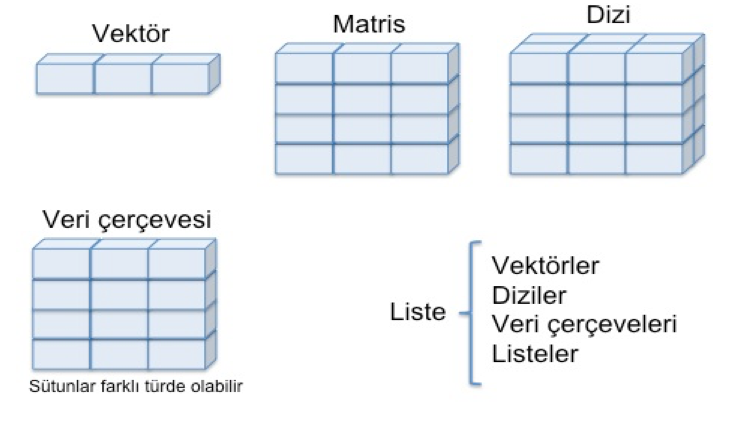
\includegraphics[width=0.8\linewidth]{B3_Sekil7} 

}

\caption{R programında yer alan veri yapıları (Kabacoff, 2011. "R in Action")}\label{fig:B3Sekil7}
\end{figure}

\subsection{Vektörler}\label{vektuxf6rler}

R programında vektörler bir dizi veri içeren tek boyutlu veri yapılarıdır. Vektörlerde bir araya getirilen veriler sayısal (tamsayı veya double), mantıksal, karakter veya kompleks olabilir. Aşağıda görüldüğü gibi R programında konsoldan girilen herhangi bir sayı bir vektör olarak yorumlanmaktadır. ``{[}1{]}'' değeri bu satırda görüntülenen ilk değerin indeksini belirtmektedir ve bu durumda vektörde sadece bir değer olduğunu göstermektedir.

\begin{Shaded}
\begin{Highlighting}[]
\DecValTok{2}
\end{Highlighting}
\end{Shaded}

\begin{verbatim}
## [1] 2
\end{verbatim}

Birden fazla eleman içeren bir vektör oluşturmak istendiğinde \texttt{c()} (combine -- birleştir) fonksiyonu kullanılmaktadır. Vektörde yer alacak her eleman \texttt{c()} fonksiyonunda (,) virgül kullanılarak ayrılmaktadır.

\begin{Shaded}
\begin{Highlighting}[]
\NormalTok{vec }\OtherTok{\textless{}{-}} \FunctionTok{c}\NormalTok{(}\DecValTok{20}\NormalTok{,}\DecValTok{1}\NormalTok{,}\DecValTok{23}\NormalTok{,}\DecValTok{8}\NormalTok{,}\DecValTok{6}\NormalTok{,}\DecValTok{25}\NormalTok{,}\DecValTok{4}\NormalTok{,}\DecValTok{19}\NormalTok{,}\DecValTok{22}\NormalTok{,}\DecValTok{16}\NormalTok{,}\DecValTok{11}\NormalTok{,}\DecValTok{17}\NormalTok{,}\DecValTok{3}\NormalTok{,}\DecValTok{18}\NormalTok{,}\DecValTok{5}\NormalTok{,}\DecValTok{24}\NormalTok{,}\DecValTok{7}\NormalTok{,}\DecValTok{15}\NormalTok{,}\DecValTok{21}\NormalTok{,}\DecValTok{12}\NormalTok{, }\DecValTok{2}\NormalTok{,}\DecValTok{10}\NormalTok{, }\DecValTok{9}\NormalTok{,}\DecValTok{13}\NormalTok{,}\DecValTok{14}\NormalTok{)}
\NormalTok{vec}
\end{Highlighting}
\end{Shaded}

\begin{verbatim}
##  [1] 20  1 23  8  6 25  4 19 22 16 11 17  3 18  5 24  7 15 21 12  2 10  9 13 14
\end{verbatim}

\begin{Shaded}
\begin{Highlighting}[]
\FunctionTok{typeof}\NormalTok{(vec)}
\end{Highlighting}
\end{Shaded}

\begin{verbatim}
## [1] "double"
\end{verbatim}

Vektör yapısında tanımlanan vec isimli değişken 25 eleman içermektedir. Listelenen değerlerin sol tarafında {[} {]} içerisinde verilen değerler ({[}1{]} ve {[}14{]}) her bir satırda sıralanan 20 ve 18 değerlerinin indeksini belirtmektedir. R programında indeksler her zaman 1'den başlar. R programında \texttt{vec} vektörünün 12. elemanını veya 10. elemandan 12. elemana kadarki değerleri elde etmek için aşağıdaki şekilde işlem yapılmalıdır.

\begin{Shaded}
\begin{Highlighting}[]
\NormalTok{vec }\OtherTok{\textless{}{-}} \FunctionTok{c}\NormalTok{(}\DecValTok{20}\NormalTok{,}\DecValTok{1}\NormalTok{,}\DecValTok{23}\NormalTok{,}\DecValTok{8}\NormalTok{,}\DecValTok{6}\NormalTok{,}\DecValTok{25}\NormalTok{,}\DecValTok{4}\NormalTok{,}\DecValTok{19}\NormalTok{,}\DecValTok{22}\NormalTok{,}\DecValTok{16}\NormalTok{,}\DecValTok{11}\NormalTok{,}\DecValTok{17}\NormalTok{,}\DecValTok{3}\NormalTok{,}\DecValTok{18}\NormalTok{,}\DecValTok{5}\NormalTok{,}\DecValTok{24}\NormalTok{,}\DecValTok{7}\NormalTok{,}\DecValTok{15}\NormalTok{,}\DecValTok{21}\NormalTok{,}\DecValTok{12}\NormalTok{, }\DecValTok{2}\NormalTok{,}\DecValTok{10}\NormalTok{, }\DecValTok{9}\NormalTok{,}\DecValTok{13}\NormalTok{,}\DecValTok{14}\NormalTok{)}
\NormalTok{vec}
\end{Highlighting}
\end{Shaded}

\begin{verbatim}
##  [1] 20  1 23  8  6 25  4 19 22 16 11 17  3 18  5 24  7 15 21 12  2 10  9 13 14
\end{verbatim}

\begin{Shaded}
\begin{Highlighting}[]
\NormalTok{vec[}\DecValTok{12}\NormalTok{]}
\end{Highlighting}
\end{Shaded}

\begin{verbatim}
## [1] 17
\end{verbatim}

\begin{Shaded}
\begin{Highlighting}[]
\NormalTok{vec[}\DecValTok{10}\SpecialCharTok{:}\DecValTok{12}\NormalTok{]}
\end{Highlighting}
\end{Shaded}

\begin{verbatim}
## [1] 16 11 17
\end{verbatim}

NOT: Vektör oluştururken, vektörde yer alan tüm verilerin aynı tipte olmasına dikkat edilmelidir. Eğer vektörde yer alan veriler içerisinde karakter olarak tanımlanan herhangi bir değer yer alırsa, R programı bu vektörü aşağıda verilen \texttt{x\ vektörü} gibi karakter veri türünde tanımlayacaktır.

\begin{Shaded}
\begin{Highlighting}[]
\NormalTok{x }\OtherTok{\textless{}{-}} \FunctionTok{c}\NormalTok{(}\DecValTok{1}\NormalTok{,}\DecValTok{2}\NormalTok{,}\StringTok{"a"}\NormalTok{)}
\NormalTok{x}
\end{Highlighting}
\end{Shaded}

\begin{verbatim}
## [1] "1" "2" "a"
\end{verbatim}

\begin{Shaded}
\begin{Highlighting}[]
\FunctionTok{typeof}\NormalTok{(x)}
\end{Highlighting}
\end{Shaded}

\begin{verbatim}
## [1] "character"
\end{verbatim}

\subsection{Matrisler}\label{matrisler}

R programında matrisler bir dizi veri içeren iki (satır ve sütun) boyutlu veri yapılarıdır. Matrislerde bir araya getirilen veriler sayısal (tamsayı veya double), mantıksal, karakter veya kompleks olabilir. R programında matrisler, \texttt{matrix(değerler,\ satır\ sayısı,\ sütun\ sayısı)} fonksiyonuyla oluşturulur. Matrisler tek boyutlu vektörlerden oluşturulduğundan matrisin satır ve sütun bilgilerinin belirtilmesi gerekir. Ayrıca, matrisin değerleri satır satır yerleştirilecek ise \texttt{byrow\ =\ TRUE} komutu da kullanılmalıdır. Komut \texttt{byrow\ =\ FALSE} olduğunda matrisin alacağı değerler sütun sütun yerleştirilecektir. R programında matrisler ve matris işlemleriyle ilgili detaylı bilgiler Bölüm IV`de verilmiştir.

\begin{Shaded}
\begin{Highlighting}[]
\NormalTok{matris }\OtherTok{\textless{}{-}} \FunctionTok{matrix}\NormalTok{(}\FunctionTok{c}\NormalTok{(}\DecValTok{1}\NormalTok{, }\DecValTok{2}\NormalTok{, }\DecValTok{3}\NormalTok{, }\DecValTok{4}\NormalTok{, }\DecValTok{5}\NormalTok{, }\DecValTok{6}\NormalTok{), }\AttributeTok{nrow =} \DecValTok{3}\NormalTok{, }\AttributeTok{ncol =} \DecValTok{2}\NormalTok{, }\AttributeTok{byrow =} \ConstantTok{TRUE}\NormalTok{)}
\NormalTok{matris}
\end{Highlighting}
\end{Shaded}

\begin{verbatim}
##      [,1] [,2]
## [1,]    1    2
## [2,]    3    4
## [3,]    5    6
\end{verbatim}

\begin{Shaded}
\begin{Highlighting}[]
\FunctionTok{typeof}\NormalTok{(matris)}
\end{Highlighting}
\end{Shaded}

\begin{verbatim}
## [1] "double"
\end{verbatim}

\subsection{Diziler}\label{diziler}

R programında diziler bir veya birden fazla aynı boyutta matris içeren çok boyutlu veri yapılarıdır. Matris ve vektörlerde olduğu gibi dizilerin elemanları aynı tipten (sayısal, mantıksal, karakter veya kompleks) olmalıdır. R programında diziler, \texttt{array(veri,\ dim=c(satır\ sayısı,\ sütun\ sayısı,\ matris\ sayısı),\ dimnames=NULL)} fonksiyonuyla oluşturulur. Fonksiyonda, \texttt{veri}: dizi değerlerini oluşturacak vektörü, \texttt{dim}: dizide yer alacak matrislerin boyutunu ve matris sayısını ve \texttt{dimnames}: boyutların isimlerini belirtir.

\begin{Shaded}
\begin{Highlighting}[]
\CommentTok{\# 2x3 boyutunda 2 matris (N ve M) içeren w dizi değişkeni}
\NormalTok{w }\OtherTok{\textless{}{-}} \FunctionTok{array}\NormalTok{(}\DecValTok{1}\SpecialCharTok{:}\DecValTok{12}\NormalTok{, }\AttributeTok{dim=}\FunctionTok{c}\NormalTok{(}\DecValTok{2}\NormalTok{,}\DecValTok{3}\NormalTok{,}\DecValTok{2}\NormalTok{), }
           \AttributeTok{dimnames=}\FunctionTok{list}\NormalTok{(}\FunctionTok{c}\NormalTok{(}\StringTok{"A"}\NormalTok{,}\StringTok{"B"}\NormalTok{), }\FunctionTok{c}\NormalTok{(}\StringTok{"X"}\NormalTok{,}\StringTok{"Y"}\NormalTok{,}\StringTok{"Z"}\NormalTok{), }\FunctionTok{c}\NormalTok{(}\StringTok{"N"}\NormalTok{,}\StringTok{"M"}\NormalTok{))) }
\NormalTok{w}
\end{Highlighting}
\end{Shaded}

\begin{verbatim}
## , , N
## 
##   X Y Z
## A 1 3 5
## B 2 4 6
## 
## , , M
## 
##   X  Y  Z
## A 7  9 11
## B 8 10 12
\end{verbatim}

Matematiksel ifadelerde diziler kullanıldığında, vektör ve matrislerde olduğu gibi işlemler element element gerçekleştirilir.

\begin{Shaded}
\begin{Highlighting}[]
\NormalTok{w }\OtherTok{\textless{}{-}} \FunctionTok{array}\NormalTok{(}\DecValTok{1}\SpecialCharTok{:}\DecValTok{12}\NormalTok{, }\AttributeTok{dim=}\FunctionTok{c}\NormalTok{(}\DecValTok{2}\NormalTok{,}\DecValTok{3}\NormalTok{,}\DecValTok{2}\NormalTok{), }
           \AttributeTok{dimnames=}\FunctionTok{list}\NormalTok{(}\FunctionTok{c}\NormalTok{(}\StringTok{"A"}\NormalTok{,}\StringTok{"B"}\NormalTok{), }\FunctionTok{c}\NormalTok{(}\StringTok{"X"}\NormalTok{,}\StringTok{"Y"}\NormalTok{,}\StringTok{"Z"}\NormalTok{), }\FunctionTok{c}\NormalTok{(}\StringTok{"N"}\NormalTok{,}\StringTok{"M"}\NormalTok{))) }
\CommentTok{\# w dizisinde yer alan 1. matrisin 2. satır ve 3. sütununda bulunan değer}
\NormalTok{w[}\DecValTok{2}\NormalTok{, }\DecValTok{3}\NormalTok{, }\DecValTok{1}\NormalTok{]}
\end{Highlighting}
\end{Shaded}

\begin{verbatim}
## [1] 6
\end{verbatim}

\begin{Shaded}
\begin{Highlighting}[]
\CommentTok{\# w dizisindeki N ve M matrislerindeki Y sütunda bulunan değerler}
\NormalTok{w[ , }\StringTok{"Y"}\NormalTok{, ]}
\end{Highlighting}
\end{Shaded}

\begin{verbatim}
##   N  M
## A 3  9
## B 4 10
\end{verbatim}

\begin{Shaded}
\begin{Highlighting}[]
\CommentTok{\# w dizisindeki M matrisindeki 1. ve 2. satırında bulunan değerler}
\NormalTok{w[}\DecValTok{1}\SpecialCharTok{:}\DecValTok{2}\NormalTok{, ,}\StringTok{"M"}\NormalTok{] }
\end{Highlighting}
\end{Shaded}

\begin{verbatim}
##   X  Y  Z
## A 7  9 11
## B 8 10 12
\end{verbatim}

\subsection{Listeler}\label{listeler}

R programında listeler dizilerin daha genel bir formu olup, farklı veri tipinde ve boyutta elemanlara (vektör, matris vb.) sahip olan veri yapılarıdır. \texttt{list()} fonksiyonu kullanılarak istenilen tüm aynı veya farklı türde ve boyutta olan veri yapıları liste veri yapısı bünyesinde bir araya getirilebilir. Aşağıda verilen örnekte \texttt{num} sayısal vektörü, ``\texttt{Ali}'' karakter değişkeni ve 2x2 boyutundaki identity matrisi \texttt{x} listesi içerisinde bir araya getirilmiştir.

\begin{Shaded}
\begin{Highlighting}[]
\NormalTok{x }\OtherTok{\textless{}{-}} \FunctionTok{list}\NormalTok{(}\AttributeTok{num=}\FunctionTok{c}\NormalTok{(}\DecValTok{1}\NormalTok{, }\DecValTok{2}\NormalTok{, }\DecValTok{3}\NormalTok{), }\StringTok{"Ali"}\NormalTok{, }\AttributeTok{identity=}\FunctionTok{diag}\NormalTok{(}\DecValTok{2}\NormalTok{)) }
\NormalTok{x}
\end{Highlighting}
\end{Shaded}

\begin{verbatim}
## $num
## [1] 1 2 3
## 
## [[2]]
## [1] "Ali"
## 
## $identity
##      [,1] [,2]
## [1,]    1    0
## [2,]    0    1
\end{verbatim}

\begin{Shaded}
\begin{Highlighting}[]
\FunctionTok{typeof}\NormalTok{(x)}
\end{Highlighting}
\end{Shaded}

\begin{verbatim}
## [1] "list"
\end{verbatim}

Listenin elemanlarına ulaşabilmek için {[} {]}, {[}{[} {]}{]} ve \$ işareti kullanılabilir

\begin{Shaded}
\begin{Highlighting}[]
\NormalTok{x }\OtherTok{\textless{}{-}} \FunctionTok{list}\NormalTok{(}\AttributeTok{num=}\FunctionTok{c}\NormalTok{(}\DecValTok{1}\NormalTok{, }\DecValTok{2}\NormalTok{, }\DecValTok{3}\NormalTok{), }\StringTok{"Ali"}\NormalTok{, }\AttributeTok{identity=}\FunctionTok{diag}\NormalTok{(}\DecValTok{2}\NormalTok{)) }
\NormalTok{x}
\end{Highlighting}
\end{Shaded}

\begin{verbatim}
## $num
## [1] 1 2 3
## 
## [[2]]
## [1] "Ali"
## 
## $identity
##      [,1] [,2]
## [1,]    1    0
## [2,]    0    1
\end{verbatim}

\begin{Shaded}
\begin{Highlighting}[]
\CommentTok{\# x listesinin ikinci elemanı}
\NormalTok{x[[}\DecValTok{2}\NormalTok{]]}
\end{Highlighting}
\end{Shaded}

\begin{verbatim}
## [1] "Ali"
\end{verbatim}

\begin{Shaded}
\begin{Highlighting}[]
\CommentTok{\# x listesinin “num” isimli elemanı}
\NormalTok{x[[}\StringTok{"num"}\NormalTok{]]             }
\end{Highlighting}
\end{Shaded}

\begin{verbatim}
## [1] 1 2 3
\end{verbatim}

\begin{Shaded}
\begin{Highlighting}[]
\CommentTok{\# x listesinin “identity” isimli elemanı}
\NormalTok{x}\SpecialCharTok{$}\NormalTok{identity             }
\end{Highlighting}
\end{Shaded}

\begin{verbatim}
##      [,1] [,2]
## [1,]    1    0
## [2,]    0    1
\end{verbatim}

\begin{Shaded}
\begin{Highlighting}[]
\CommentTok{\# x listesinin 3. elemanının 1. satırı}
\NormalTok{x[[}\DecValTok{3}\NormalTok{]][}\DecValTok{1}\NormalTok{,]}
\end{Highlighting}
\end{Shaded}

\begin{verbatim}
## [1] 1 0
\end{verbatim}

\begin{Shaded}
\begin{Highlighting}[]
\CommentTok{\# x listesinin ilk iki elemanından oluşan bir alt liste}
\NormalTok{x[}\DecValTok{1}\SpecialCharTok{:}\DecValTok{2}\NormalTok{]}
\end{Highlighting}
\end{Shaded}

\begin{verbatim}
## $num
## [1] 1 2 3
## 
## [[2]]
## [1] "Ali"
\end{verbatim}

\subsection{Faktörler}\label{faktuxf6rler}

R programında faktörler, bir dizi karakter veya tamsayı veri tipinde kategorik veri içeren tek boyutlu veri yapılarıdır. \texttt{factor()} fonksiyonu kullanılarak mevcut veriler, faktör veri yapısına dönüştürülebilir ve birbirinden farklı eleman sayısı \texttt{nlevels()} fonksiyonu kullanılarak belirlenebilir. Faktör veri yapısı istatistiksel analizlerde değişken tanımlamada çok kullanılan yapılardır.

\begin{Shaded}
\begin{Highlighting}[]
\NormalTok{degisken }\OtherTok{\textless{}{-}} \FunctionTok{c}\NormalTok{(}\StringTok{"ahmet"}\NormalTok{,}\StringTok{"mehmet"}\NormalTok{,}\StringTok{"ali"}\NormalTok{,}\StringTok{"ahmet"}\NormalTok{,}\StringTok{"ahmet"}\NormalTok{,}\StringTok{"ali"}\NormalTok{,}\StringTok{"veli"}\NormalTok{,}\StringTok{"mehmet"}\NormalTok{)}
\NormalTok{factor\_degisken }\OtherTok{\textless{}{-}} \FunctionTok{factor}\NormalTok{(degisken)}
\NormalTok{factor\_degisken}
\end{Highlighting}
\end{Shaded}

\begin{verbatim}
## [1] ahmet  mehmet ali    ahmet  ahmet  ali    veli   mehmet
## Levels: ahmet ali mehmet veli
\end{verbatim}

\begin{Shaded}
\begin{Highlighting}[]
\FunctionTok{nlevels}\NormalTok{(factor\_degisken)}
\end{Highlighting}
\end{Shaded}

\begin{verbatim}
## [1] 4
\end{verbatim}

R programda \texttt{gl(n,\ k,\ labels)} fonksiyonu kullanılarak faktör veri yapısında değişkenler oluşturulabilir. Bu fonksiyonda \texttt{n}: tam sayı olmalıdır ve faktör değişkenindeki seviye sayısını, \texttt{k}: tam sayı olmalıdır ve faktör değişkenindeki seviyelerin tekrar sayısını ve \texttt{labels}: faktör değişkeninde yer alan seviyelerin etiketlerinin içeren bir vektörü belirtmektedir.

\begin{Shaded}
\begin{Highlighting}[]
\NormalTok{grup }\OtherTok{=} \FunctionTok{gl}\NormalTok{(}\DecValTok{2}\NormalTok{, }\DecValTok{5}\NormalTok{, }\AttributeTok{labels =} \FunctionTok{c}\NormalTok{(}\StringTok{"A"}\NormalTok{, }\StringTok{"B"}\NormalTok{))}
\NormalTok{grup}
\end{Highlighting}
\end{Shaded}

\begin{verbatim}
##  [1] A A A A A B B B B B
## Levels: A B
\end{verbatim}

\subsection{Veri Çerçeveleri}\label{veri-uxe7eruxe7eveleri}

R programında veri çerçeveleri matrisler gibi iki boyutlu olup farklı veri tiplerini (sayısal, mantıksal, karakter veya kompleks) aynı boyutta vektörler (sütunlar) halinde bünyesinde bulunduran veri yapılarıdır. Veri çerçeveleri aynı zamanda aşağıda verilen örnekte de olduğu gibi aynı veya farklı veri tiplerinin (değişkenlerin) tablo halinde bir araya getirilmesi olarak da düşünülebilir. \texttt{data.frame()} fonksiyonu kullanılarak, veri tiplerine bakılmaksızın boyutları aynı olan vektörler tablo formatında veri çerçevesi olarak bir araya getirilebilir.

\begin{Shaded}
\begin{Highlighting}[]
\NormalTok{isim }\OtherTok{=} \FunctionTok{c}\NormalTok{(}\StringTok{"Ahmet"}\NormalTok{,}\StringTok{"Mehmet"}\NormalTok{,}\StringTok{"Veli"}\NormalTok{)}
\NormalTok{satislari }\OtherTok{=} \FunctionTok{c}\NormalTok{(}\DecValTok{120000}\NormalTok{,}\DecValTok{140000}\NormalTok{,}\DecValTok{100000}\NormalTok{)}
\NormalTok{karoranlari }\OtherTok{=} \FunctionTok{c}\NormalTok{(}\FloatTok{25.5}\NormalTok{,}\DecValTok{22}\NormalTok{,}\FloatTok{38.75}\NormalTok{)}
\NormalTok{aktifdurumlari }\OtherTok{=} \FunctionTok{c}\NormalTok{(}\StringTok{"Evet"}\NormalTok{,}\StringTok{"Hayir"}\NormalTok{,}\StringTok{"Evet"}\NormalTok{)}

\NormalTok{FinansVerileri }\OtherTok{\textless{}{-}} \FunctionTok{data.frame}\NormalTok{(isim, satislari, karoranlari, aktifdurumlari)}
\NormalTok{FinansVerileri}
\end{Highlighting}
\end{Shaded}

\begin{verbatim}
##     isim satislari karoranlari aktifdurumlari
## 1  Ahmet    120000       25.50           Evet
## 2 Mehmet    140000       22.00          Hayir
## 3   Veli    100000       38.75           Evet
\end{verbatim}

Yukarıda oluşturulan \texttt{FinansVerileri} veri çerçevesinde olduğu gibi R programında veri çerçevelerinde:

\begin{itemize}
\tightlist
\item
  Sütun isimleri R programında değişken isimleri için geçerli olan kurallar dikkate alınarak oluşturulmalı ve boş bırakılmamalıdır
\item
  Satır isimleri de farklı olmalıdır
\item
  Veri çerçevesinde oluşturulan veri seti sayısal, mantıksal, karakter veya kompleks veri tiplerini sütunlar halinde karışı olarak içerebilir
\item
  Veri çerçevelerinde her sütun aynı boyutta veri içermelidir
  Veri çerçevelerindeki sütun değerlerine veya bireysel değerlere ulaşabilmek için {[} {]} veya \$ işareti kullanılabilir.
\end{itemize}

\begin{Shaded}
\begin{Highlighting}[]
\NormalTok{isim }\OtherTok{=} \FunctionTok{c}\NormalTok{(}\StringTok{"Ahmet"}\NormalTok{,}\StringTok{"Mehmet"}\NormalTok{,}\StringTok{"Veli"}\NormalTok{)}
\NormalTok{satislari }\OtherTok{=} \FunctionTok{c}\NormalTok{(}\DecValTok{120000}\NormalTok{,}\DecValTok{140000}\NormalTok{,}\DecValTok{100000}\NormalTok{)}
\NormalTok{karoranlari }\OtherTok{=} \FunctionTok{c}\NormalTok{(}\FloatTok{25.5}\NormalTok{,}\DecValTok{22}\NormalTok{,}\FloatTok{38.75}\NormalTok{)}
\NormalTok{aktifdurumlari }\OtherTok{=} \FunctionTok{c}\NormalTok{(}\StringTok{"Evet"}\NormalTok{,}\StringTok{"Hayir"}\NormalTok{,}\StringTok{"Evet"}\NormalTok{)}

\NormalTok{FinansVerileri }\OtherTok{\textless{}{-}} \FunctionTok{data.frame}\NormalTok{(isim, satislari, karoranlari, aktifdurumlari)}
\NormalTok{FinansVerileri}
\end{Highlighting}
\end{Shaded}

\begin{verbatim}
##     isim satislari karoranlari aktifdurumlari
## 1  Ahmet    120000       25.50           Evet
## 2 Mehmet    140000       22.00          Hayir
## 3   Veli    100000       38.75           Evet
\end{verbatim}

\begin{Shaded}
\begin{Highlighting}[]
\CommentTok{\# FinansVerileri veri çerçevesinde sütunun değerleri aşağıda verilen farklı şekillerde elde edilebilir }
\NormalTok{FinansVerileri[}\DecValTok{1}\NormalTok{]}
\end{Highlighting}
\end{Shaded}

\begin{verbatim}
##     isim
## 1  Ahmet
## 2 Mehmet
## 3   Veli
\end{verbatim}

\begin{Shaded}
\begin{Highlighting}[]
\NormalTok{FinansVerileri[,}\DecValTok{1}\NormalTok{]}
\end{Highlighting}
\end{Shaded}

\begin{verbatim}
## [1] "Ahmet"  "Mehmet" "Veli"
\end{verbatim}

\begin{Shaded}
\begin{Highlighting}[]
\NormalTok{FinansVerileri}\SpecialCharTok{$}\NormalTok{isim}
\end{Highlighting}
\end{Shaded}

\begin{verbatim}
## [1] "Ahmet"  "Mehmet" "Veli"
\end{verbatim}

\begin{Shaded}
\begin{Highlighting}[]
\CommentTok{\# FinansVerileri veri çerçevesinde gözlem değerleri aşağıda verilen farklı şekillerde elde edilebilir }
\NormalTok{FinansVerileri[}\DecValTok{1}\NormalTok{,}\DecValTok{2}\NormalTok{]}
\end{Highlighting}
\end{Shaded}

\begin{verbatim}
## [1] 120000
\end{verbatim}

\begin{Shaded}
\begin{Highlighting}[]
\NormalTok{FinansVerileri}\SpecialCharTok{$}\NormalTok{satislari[}\DecValTok{1}\NormalTok{]}
\end{Highlighting}
\end{Shaded}

\begin{verbatim}
## [1] 120000
\end{verbatim}

\section{\texorpdfstring{Çıktıların Yazdırılması \texttt{print()} ve \texttt{cat()} Fonksiyonları}{Çıktıların Yazdırılması print() ve cat() Fonksiyonları}}\label{uxe7ux131ktux131larux131n-yazdux131rux131lmasux131-print-ve-cat-fonksiyonlarux131}

R programında çıktıların veya nesnelerin ekrana veya dosyaya yazdırılmasında \texttt{print()} veya \texttt{cat()} fonksiyonları kullanılır.

\subsection{print() Fonksiyonu}\label{print-fonksiyonu}

R programında oluşturulan farklı veya aynı veri tiplerini (sayısal, mantıksal, karakter veya kompleks) içeren veri yapıları veya analiz çıktıları \texttt{print()} fonksiyonu ile yazdırılabilir.

\begin{Shaded}
\begin{Highlighting}[]
\CommentTok{\# "Merhaba dünya" ifadesi " " içerisinde ekrana yazdırılmaktadır}
\FunctionTok{print}\NormalTok{(}\StringTok{"Merhaba dünya"}\NormalTok{)}
\end{Highlighting}
\end{Shaded}

\begin{verbatim}
## [1] "Merhaba dünya"
\end{verbatim}

\begin{Shaded}
\begin{Highlighting}[]
\CommentTok{\# B numerik nesnesinin ekrana yazdırılması}
\NormalTok{B }\OtherTok{\textless{}{-}} \DecValTok{3} \SpecialCharTok{+} \DecValTok{5}
\FunctionTok{print}\NormalTok{(B)}
\end{Highlighting}
\end{Shaded}

\begin{verbatim}
## [1] 8
\end{verbatim}

\begin{Shaded}
\begin{Highlighting}[]
\CommentTok{\# B numerik nesnesinin paste() fonksiyonu ile ekrana yazdırılması}
\NormalTok{B }\OtherTok{\textless{}{-}} \DecValTok{3} \SpecialCharTok{+} \DecValTok{5}
\FunctionTok{print}\NormalTok{(}\FunctionTok{paste}\NormalTok{(}\StringTok{"B değişkeninin değeri: "}\NormalTok{, B))}
\end{Highlighting}
\end{Shaded}

\begin{verbatim}
## [1] "B değişkeninin değeri:  8"
\end{verbatim}

\begin{Shaded}
\begin{Highlighting}[]
\CommentTok{\# A matrisi de matris formatında ekrana yazdırılmaktadır}
\NormalTok{A }\OtherTok{\textless{}{-}} \FunctionTok{matrix}\NormalTok{(}\DecValTok{1}\SpecialCharTok{:}\DecValTok{9}\NormalTok{, }\DecValTok{3}\NormalTok{, }\DecValTok{3}\NormalTok{)}
\FunctionTok{print}\NormalTok{(A)}
\end{Highlighting}
\end{Shaded}

\begin{verbatim}
##      [,1] [,2] [,3]
## [1,]    1    4    7
## [2,]    2    5    8
## [3,]    3    6    9
\end{verbatim}

\begin{Shaded}
\begin{Highlighting}[]
\CommentTok{\# insan veri seti de ekrana data.frame formatında yazdırılmaktadır}
\NormalTok{insan }\OtherTok{\textless{}{-}} \FunctionTok{data.frame}\NormalTok{(}\AttributeTok{No=}\FunctionTok{c}\NormalTok{(}\DecValTok{1}\SpecialCharTok{:}\DecValTok{5}\NormalTok{), }
                    \AttributeTok{Cinsiyet=}\FunctionTok{c}\NormalTok{(}\StringTok{"Erkek"}\NormalTok{,}\StringTok{"Dişi"}\NormalTok{,}\StringTok{"Erkek"}\NormalTok{,}\StringTok{"Dişi"}\NormalTok{,}\StringTok{"Dişi"}\NormalTok{),}
                    \AttributeTok{Boy=}\FunctionTok{c}\NormalTok{(}\DecValTok{190}\NormalTok{, }\DecValTok{170}\NormalTok{, }\DecValTok{175}\NormalTok{, }\DecValTok{180}\NormalTok{, }\DecValTok{173}\NormalTok{))}
\FunctionTok{print}\NormalTok{(insan)}
\end{Highlighting}
\end{Shaded}

\begin{verbatim}
##   No Cinsiyet Boy
## 1  1    Erkek 190
## 2  2     Dişi 170
## 3  3    Erkek 175
## 4  4     Dişi 180
## 5  5     Dişi 173
\end{verbatim}

\subsection{cat() Fonksiyonu}\label{cat-fonksiyonu}

R programında, sayısal, mantıksal, karakter veya kompleks veri tipinde oluşturulan değişkenler \texttt{cat()} fonksiyonu ile yazdırılabilir. \texttt{cat()} fonksiyonu ile arka arkaya iki satırda yazdırılmak istenen ifadeler olduğunda, birleştirerek yazdırılmaktadır. Bunu önlemek ve yeni satıra yazdırmak için \texttt{cat()} içerisindeki ifadenin sonuna ``\texttt{\textbackslash{}n}'' eklenmelidir. \texttt{cat()} fonksiyonu içerisinde \texttt{paste()} fonksiyonu kullanılarak da ifadeler birleştirilerek yazdırılabilir.

\begin{Shaded}
\begin{Highlighting}[]
\CommentTok{\# "Merhaba dünya" ifadesi " " olmadan ekrana yazdırılmaktadır}
\FunctionTok{cat}\NormalTok{(}\StringTok{"Merhaba dünya }\SpecialCharTok{\textbackslash{}n}\StringTok{"}\NormalTok{)}
\end{Highlighting}
\end{Shaded}

\begin{verbatim}
## Merhaba dünya
\end{verbatim}

\begin{Shaded}
\begin{Highlighting}[]
\CommentTok{\# B numerik nesnesinin ekrana yazdırılması}
\NormalTok{B }\OtherTok{\textless{}{-}} \DecValTok{3} \SpecialCharTok{+} \DecValTok{5}
\FunctionTok{cat}\NormalTok{(B, }\StringTok{"}\SpecialCharTok{\textbackslash{}n}\StringTok{"}\NormalTok{)}
\end{Highlighting}
\end{Shaded}

\begin{verbatim}
## 8
\end{verbatim}

\begin{Shaded}
\begin{Highlighting}[]
\CommentTok{\# B numerik nesnesinin paste() fonksiyonu ile ekrana yazdırılması}
\NormalTok{B }\OtherTok{\textless{}{-}} \DecValTok{3} \SpecialCharTok{+} \DecValTok{5}
\FunctionTok{cat}\NormalTok{(}\FunctionTok{paste}\NormalTok{(}\StringTok{"B değişkeninin değeri: "}\NormalTok{, B, }\StringTok{"}\SpecialCharTok{\textbackslash{}n}\StringTok{"}\NormalTok{))}
\end{Highlighting}
\end{Shaded}

\begin{verbatim}
## B değişkeninin değeri:  8
\end{verbatim}

\texttt{cat()} fonksiyonu ile matris veya veri çerçevesi gibi veri yapısında oluşturulan nesneler istenilen formatta yazdırılamamakta veya hata oluşmaktadır. Veri yapılarının yazdırılabilmesi için \texttt{print()} fonksiyonu kullanılmalıdır.

\begin{Shaded}
\begin{Highlighting}[]
\CommentTok{\# A matrisi de matris formatında ekrana yazdırılmaktadır}
\NormalTok{A }\OtherTok{\textless{}{-}} \FunctionTok{matrix}\NormalTok{(}\DecValTok{1}\SpecialCharTok{:}\DecValTok{9}\NormalTok{, }\DecValTok{3}\NormalTok{, }\DecValTok{3}\NormalTok{)}
\FunctionTok{cat}\NormalTok{(A, }\StringTok{"}\SpecialCharTok{\textbackslash{}n}\StringTok{"}\NormalTok{)}
\end{Highlighting}
\end{Shaded}

\begin{verbatim}
## 1 2 3 4 5 6 7 8 9
\end{verbatim}

\begin{Shaded}
\begin{Highlighting}[]
\CommentTok{\# insan veri seti de ekrana data.frame formatında yazdırılmaktadır}
\NormalTok{insan }\OtherTok{\textless{}{-}} \FunctionTok{data.frame}\NormalTok{(}\AttributeTok{No=}\FunctionTok{c}\NormalTok{(}\DecValTok{1}\SpecialCharTok{:}\DecValTok{5}\NormalTok{), }
                    \AttributeTok{Cinsiyet=}\FunctionTok{c}\NormalTok{(}\StringTok{"Erkek"}\NormalTok{,}\StringTok{"Dişi"}\NormalTok{,}\StringTok{"Erkek"}\NormalTok{,}\StringTok{"Dişi"}\NormalTok{,}\StringTok{"Dişi"}\NormalTok{),}
                    \AttributeTok{Boy=}\FunctionTok{c}\NormalTok{(}\DecValTok{190}\NormalTok{, }\DecValTok{170}\NormalTok{, }\DecValTok{175}\NormalTok{, }\DecValTok{180}\NormalTok{, }\DecValTok{173}\NormalTok{))}
\FunctionTok{cat}\NormalTok{(insan, }\StringTok{"}\SpecialCharTok{\textbackslash{}n}\StringTok{"}\NormalTok{)}
\end{Highlighting}
\end{Shaded}

\begin{verbatim}
## Error in cat(insan, "\n"): argument 1 (type 'list') cannot be handled by 'cat'
\end{verbatim}

\chapter{Matrisler}\label{matrisler-1}

Matrisler, sayıların veya matematiksel ifadelerin satırlar ve sütunlar halinde düzenlenmiş şekli olup \textbf{A}, \textbf{B}, \textbf{I} veya \textbf{X} gibi büyük ve koyu harflerle gösterilirlerc

\[A_{r×c} =
 \begin{pmatrix}
  a_{1,1} & a_{1,2} & \cdots & a_{1,c} \\
  a_{2,1} & a_{2,2} & \cdots & a_{2,c} \\
  \vdots  & \vdots  & \ddots & \vdots  \\
  a_{r,1} & a_{r,2} & \cdots & a_{r,c}
 \end{pmatrix}_{r × c}\]

Yukarıda verilen \textbf{A} matrisi, \emph{r satır} ve \emph{c sütundan} oluşmuştur. Matrisin sağ alt köşesinde verilen bu değerler (\emph{r × c}), matrisin boyutunu belirtir. Aşağıda verilen \textbf{M} matrisi, 3 satır ve 3 sütundan oluşan ve sayısal değerler içeren bir matristir.

\[M_{3×3} =
  \begin{pmatrix}
11 & 0.20 & 13 \\
47 & 35 & 6.7 \\
0.70 & 18 & 29 
\end{pmatrix}_{3×3}\]

R programında matrisler, \texttt{matrix(değerler,\ satır,\ sütun)} fonksiyonuyla oluşturulur. Fonksiyondan da anlaşılacağı gibi matrislerin tanımlanmasında, matrisi oluşturacak değerlerle birlikte, matrisin satır ve sütun sayılarının da belirtilmesi gerekmektedir. Buna göre, \textbf{M} matrisi, R programında aşağıdaki şekilde oluşturulup yazdırılabilir.

\begin{Shaded}
\begin{Highlighting}[]
\NormalTok{M }\OtherTok{\textless{}{-}} \FunctionTok{matrix}\NormalTok{(}\FunctionTok{c}\NormalTok{(}\DecValTok{11}\NormalTok{,}\DecValTok{47}\NormalTok{,}\DecValTok{7}\NormalTok{,}\DecValTok{20}\NormalTok{,}\DecValTok{35}\NormalTok{,}\DecValTok{18}\NormalTok{,}\DecValTok{13}\NormalTok{,}\DecValTok{67}\NormalTok{,}\DecValTok{29}\NormalTok{), }\DecValTok{3}\NormalTok{, }\DecValTok{3}\NormalTok{) }
\NormalTok{M }
\end{Highlighting}
\end{Shaded}

\begin{verbatim}
##      [,1] [,2] [,3]
## [1,]   11   20   13
## [2,]   47   35   67
## [3,]    7   18   29
\end{verbatim}

\textbf{M} matrisinin oluşturulmasından da anlaşılacağı gibi matrisin elemanları, birinci sütundan başlayarak yerleştirilmiştir. R programında herhangi bir tanımlama yapılmadığı zaman; değerler matrise birinci sütundan itibaren sütun sütun yerleştirilir. Matrisin elemanları satır olarak yerleştirilmek istendiğinde, \texttt{byrow=TRUE} komutu matris fonksiyonu içerisinde kullanılmalıdır. Buna göre oluşturulan \textbf{M} matrisi aşağıda verilmiştir.

\begin{Shaded}
\begin{Highlighting}[]
\NormalTok{M }\OtherTok{\textless{}{-}} \FunctionTok{matrix}\NormalTok{(}\FunctionTok{c}\NormalTok{(}\DecValTok{11}\NormalTok{,}\DecValTok{47}\NormalTok{,}\DecValTok{7}\NormalTok{,}\DecValTok{20}\NormalTok{,}\DecValTok{35}\NormalTok{,}\DecValTok{18}\NormalTok{,}\DecValTok{13}\NormalTok{,}\DecValTok{67}\NormalTok{,}\DecValTok{29}\NormalTok{), }\DecValTok{3}\NormalTok{, }\DecValTok{3}\NormalTok{, }\AttributeTok{byrow=}\ConstantTok{TRUE}\NormalTok{) }
\NormalTok{M }
\end{Highlighting}
\end{Shaded}

\begin{verbatim}
##      [,1] [,2] [,3]
## [1,]   11   47    7
## [2,]   20   35   18
## [3,]   13   67   29
\end{verbatim}

R programında tanımlanmış bir değişkenin matris olarak tanımlanıp tanımlanmadığını anlamak için aşağıda verilen bu matris mi anlamına gelen \texttt{is.matrix()} komutu kullanılabilir.

\begin{Shaded}
\begin{Highlighting}[]
\NormalTok{M }\OtherTok{\textless{}{-}} \FunctionTok{matrix}\NormalTok{(}\FunctionTok{c}\NormalTok{(}\DecValTok{11}\NormalTok{,}\DecValTok{47}\NormalTok{,}\DecValTok{7}\NormalTok{,}\DecValTok{20}\NormalTok{,}\DecValTok{35}\NormalTok{,}\DecValTok{18}\NormalTok{,}\DecValTok{13}\NormalTok{,}\DecValTok{67}\NormalTok{,}\DecValTok{29}\NormalTok{), }\DecValTok{3}\NormalTok{, }\DecValTok{3}\NormalTok{, }\AttributeTok{byrow=}\ConstantTok{TRUE}\NormalTok{) }
\FunctionTok{is.matrix}\NormalTok{(M)}
\end{Highlighting}
\end{Shaded}

\begin{verbatim}
## [1] TRUE
\end{verbatim}

Bu komutun \texttt{TRUE} veya \texttt{FALSE} olarak iki sonucu vardır. \textbf{M} değişkeninin matris olduğunu belirten \texttt{TRUE} sonucu yukarıda elde edilmiştir. \textbf{M} değişkeni farklı bir değişken olarak tanımlanmış olsaydı sonuç \texttt{FALSE} olacaktı. Ayrıca, her hangi bir matrisin boyutunu öğrenmek için \texttt{dim()} komutu, satır veya sütun sayısını öğrenmek için de \texttt{nrow()} veya \texttt{ncol()} komutu kullanılabilir.

\begin{Shaded}
\begin{Highlighting}[]
\NormalTok{M }\OtherTok{\textless{}{-}} \FunctionTok{matrix}\NormalTok{(}\FunctionTok{c}\NormalTok{(}\DecValTok{11}\NormalTok{,}\DecValTok{47}\NormalTok{,}\DecValTok{7}\NormalTok{,}\DecValTok{20}\NormalTok{,}\DecValTok{35}\NormalTok{,}\DecValTok{18}\NormalTok{,}\DecValTok{13}\NormalTok{,}\DecValTok{67}\NormalTok{,}\DecValTok{29}\NormalTok{), }\DecValTok{3}\NormalTok{, }\DecValTok{3}\NormalTok{, }\AttributeTok{byrow=}\ConstantTok{TRUE}\NormalTok{) }
\NormalTok{boyut }\OtherTok{\textless{}{-}} \FunctionTok{dim}\NormalTok{(M)         }\CommentTok{\# M matrisinin boyutu }
\NormalTok{boyut }
\end{Highlighting}
\end{Shaded}

\begin{verbatim}
## [1] 3 3
\end{verbatim}

\begin{Shaded}
\begin{Highlighting}[]
\NormalTok{satir }\OtherTok{\textless{}{-}} \FunctionTok{nrow}\NormalTok{(M)        }\CommentTok{\# M matrisinin satır sayısı }
\NormalTok{satir }
\end{Highlighting}
\end{Shaded}

\begin{verbatim}
## [1] 3
\end{verbatim}

\begin{Shaded}
\begin{Highlighting}[]
\NormalTok{sutun }\OtherTok{\textless{}{-}} \FunctionTok{ncol}\NormalTok{(M)        }\CommentTok{\# M matrisinin sütun sayısı }
\NormalTok{sutun }
\end{Highlighting}
\end{Shaded}

\begin{verbatim}
## [1] 3
\end{verbatim}

R programında matrislerin bütün elemanları yazdırıldığı gibi matrisin herhangi bir elemanı, satırı veya sütunu da yazdırılabilir. Örneğin, \textbf{M} matrisinin \(`m_{12}`\) elemanı

\begin{Shaded}
\begin{Highlighting}[]
\NormalTok{M }\OtherTok{\textless{}{-}} \FunctionTok{matrix}\NormalTok{(}\FunctionTok{c}\NormalTok{(}\DecValTok{11}\NormalTok{,}\DecValTok{47}\NormalTok{,}\DecValTok{7}\NormalTok{,}\DecValTok{20}\NormalTok{,}\DecValTok{35}\NormalTok{,}\DecValTok{18}\NormalTok{,}\DecValTok{13}\NormalTok{,}\DecValTok{67}\NormalTok{,}\DecValTok{29}\NormalTok{), }\DecValTok{3}\NormalTok{, }\DecValTok{3}\NormalTok{, }\AttributeTok{byrow=}\ConstantTok{TRUE}\NormalTok{) }
\NormalTok{M[}\DecValTok{1}\NormalTok{,}\DecValTok{2}\NormalTok{]}
\end{Highlighting}
\end{Shaded}

\begin{verbatim}
## [1] 47
\end{verbatim}

M matrisinin üçüncü satırı

\begin{Shaded}
\begin{Highlighting}[]
\NormalTok{M }\OtherTok{\textless{}{-}} \FunctionTok{matrix}\NormalTok{(}\FunctionTok{c}\NormalTok{(}\DecValTok{11}\NormalTok{,}\DecValTok{47}\NormalTok{,}\DecValTok{7}\NormalTok{,}\DecValTok{20}\NormalTok{,}\DecValTok{35}\NormalTok{,}\DecValTok{18}\NormalTok{,}\DecValTok{13}\NormalTok{,}\DecValTok{67}\NormalTok{,}\DecValTok{29}\NormalTok{), }\DecValTok{3}\NormalTok{, }\DecValTok{3}\NormalTok{, }\AttributeTok{byrow=}\ConstantTok{TRUE}\NormalTok{) }
\NormalTok{M[}\DecValTok{3}\NormalTok{,]}
\end{Highlighting}
\end{Shaded}

\begin{verbatim}
## [1] 13 67 29
\end{verbatim}

veya M matrisinin ikinci sütunu

\begin{Shaded}
\begin{Highlighting}[]
\NormalTok{M }\OtherTok{\textless{}{-}} \FunctionTok{matrix}\NormalTok{(}\FunctionTok{c}\NormalTok{(}\DecValTok{11}\NormalTok{,}\DecValTok{47}\NormalTok{,}\DecValTok{7}\NormalTok{,}\DecValTok{20}\NormalTok{,}\DecValTok{35}\NormalTok{,}\DecValTok{18}\NormalTok{,}\DecValTok{13}\NormalTok{,}\DecValTok{67}\NormalTok{,}\DecValTok{29}\NormalTok{), }\DecValTok{3}\NormalTok{, }\DecValTok{3}\NormalTok{, }\AttributeTok{byrow=}\ConstantTok{TRUE}\NormalTok{) }
\NormalTok{M[,}\DecValTok{2}\NormalTok{]}
\end{Highlighting}
\end{Shaded}

\begin{verbatim}
## [1] 47 35 67
\end{verbatim}

şeklinde yazdırılabilir. Yukarıdaki ifadelerden de anlaşılacağı gibi her hangi bir matrisin elemanları yazdırılırken veya matris işlemleri yapılırken köşeli parantez ``{[} {]}'' kullanılması gerekmektedir.

\section{Satır ve Sütun Vektörleri}\label{satux131r-ve-suxfctun-vektuxf6rleri}

Herhangi bir matris, sadece bir satırdan oluşuyorsa bu matrislere \texttt{satır\ vektörü\ (x)}

\[x_{1×c} =
\begin{pmatrix}
 x_{1,1} & x_{1,2} & \cdots & x_{1,c}
\end{pmatrix}_{1 × c}\]

veya sadece bir sütundan oluşuyorsa bu matrislere \texttt{sütun\ vektörü\ (y)} denir.

\[y_{r×1} =
\begin{pmatrix}
 y_{1,1} \\ 
 y_{2,1} \\
 \vdots \\
 y_{r,1}
\end{pmatrix}_{r×1}\]

Satır ve sütun vektörleri \textbf{a}, \textbf{b}, \textbf{x} veya \textbf{y} gibi küçük ve koyu harflerle gösterilirler. Satır ve sütun vektörlerinin oluşturulmasında yine \texttt{matrix()} komutu kullanılır. Buna göre, \textbf{a} satır vektörü aşağıdaki gibi oluşturulmuş ve boyutu da belirtilmiştir.

\[a_{1×5} =
\begin{pmatrix}
 1 & 3 & 5 & 7 & 9
\end{pmatrix}_{1 × 5}\]

\begin{Shaded}
\begin{Highlighting}[]
\NormalTok{ a }\OtherTok{\textless{}{-}} \FunctionTok{matrix}\NormalTok{(}\FunctionTok{c}\NormalTok{(}\DecValTok{1}\NormalTok{,}\DecValTok{3}\NormalTok{,}\DecValTok{5}\NormalTok{,}\DecValTok{7}\NormalTok{,}\DecValTok{9}\NormalTok{), }\DecValTok{1}\NormalTok{, }\DecValTok{5}\NormalTok{) }
\NormalTok{ a }
\end{Highlighting}
\end{Shaded}

\begin{verbatim}
##      [,1] [,2] [,3] [,4] [,5]
## [1,]    1    3    5    7    9
\end{verbatim}

\begin{Shaded}
\begin{Highlighting}[]
\NormalTok{ boyut }\OtherTok{\textless{}{-}} \FunctionTok{dim}\NormalTok{(a)}
\NormalTok{ boyut}
\end{Highlighting}
\end{Shaded}

\begin{verbatim}
## [1] 1 5
\end{verbatim}

\begin{Shaded}
\begin{Highlighting}[]
\NormalTok{ satir }\OtherTok{\textless{}{-}} \FunctionTok{nrow}\NormalTok{(a)}
\NormalTok{ satir}
\end{Highlighting}
\end{Shaded}

\begin{verbatim}
## [1] 1
\end{verbatim}

\begin{Shaded}
\begin{Highlighting}[]
\NormalTok{ sutun }\OtherTok{\textless{}{-}} \FunctionTok{ncol}\NormalTok{(a)}
\NormalTok{ sutun}
\end{Highlighting}
\end{Shaded}

\begin{verbatim}
## [1] 5
\end{verbatim}

\textbf{b} sütun vektörü de aşağıdaki gibi oluşturulmuş ve boyutu da belirtilmiştir.

\[b_{4×1} =
\begin{pmatrix}
 2 \\ 
 4 \\
 6 \\
 8
\end{pmatrix}_{4×1}\]

\begin{verbatim}
##      [,1]
## [1,]    2
## [2,]    4
## [3,]    6
## [4,]    8
\end{verbatim}

\begin{verbatim}
## [1] 4 1
\end{verbatim}

\begin{verbatim}
## [1] 4
\end{verbatim}

\begin{verbatim}
## [1] 1
\end{verbatim}

Matrislerin veya satır ve sütun vektörlerin boyutları hem bir değişkene aktarılarak hem de aktarılmadan yazdırılabilir. Hesaplama işlemlerinde matrislerin veya satır ve sütun vektörlerin boyutları kullanılacak ise bunların değişkenlere aktarılması işlemlerde kolaylık sağlayacaktır.

\section{Kare Matris}\label{kare-matris}

Satır sayısı sütun sayısına eşit olan matrislere kare matris denir. Aşağıda verilen \textbf{A} matrisi \texttt{4×4} boyutunda bir kare matristir.

\[A_{4×4} =
\begin{pmatrix}
 a_{1,1} & a_{1,2} & a_{1,3} & a_{1,4} \\
 a_{2,1} & a_{2,2} & a_{2,3} & a_{2,4} \\
 a_{3,1} & a_{3,2} & a_{3,3} & a_{3,4} \\
 a_{4,1} & a_{4,2} & a_{4,3} & a_{4,4} 
\end{pmatrix}_{4×4}\]

Matrisin sol üst köşesinden sağ alt köşesine kadar uzanan eksene, matrisin esas köşegeni veya diyagonali ve bu köşegen üzerinde yer alan \(a_{11}\), \(a_{22}\), \(a_{33}\) ve \(a_{44}\) matris elemanlarına da esas köşegen (diyagonal) elemanları denir.

R programında bir matrisin köşegen elemanları \texttt{diag()} komutu kullanılarak elde edilebilir. Buna göre, \textbf{A} ve \textbf{X} matrislerinin köşegen elemanları aşağıdaki şekilde elde edilir.

\[A_{2×2} =
  \begin{pmatrix}
10 & 30 \\
20 & 40  
\end{pmatrix}_{2×2}\]
ve

\[X_{3×3} =
  \begin{pmatrix}
1 & 2 & 3 \\
4 & 5 & 6 \\
7 & 8 & 9 \\
\end{pmatrix}_{3×3}\]

\begin{Shaded}
\begin{Highlighting}[]
\NormalTok{A }\OtherTok{\textless{}{-}} \FunctionTok{matrix}\NormalTok{(}\FunctionTok{c}\NormalTok{(}\DecValTok{10}\NormalTok{,}\DecValTok{20}\NormalTok{,}\DecValTok{30}\NormalTok{,}\DecValTok{40}\NormalTok{), }\DecValTok{2}\NormalTok{, }\DecValTok{2}\NormalTok{) }
\NormalTok{A }
\end{Highlighting}
\end{Shaded}

\begin{verbatim}
##      [,1] [,2]
## [1,]   10   30
## [2,]   20   40
\end{verbatim}

\begin{Shaded}
\begin{Highlighting}[]
\FunctionTok{diag}\NormalTok{(A)}
\end{Highlighting}
\end{Shaded}

\begin{verbatim}
## [1] 10 40
\end{verbatim}

\begin{Shaded}
\begin{Highlighting}[]
\NormalTok{X }\OtherTok{\textless{}{-}} \FunctionTok{matrix}\NormalTok{(}\FunctionTok{c}\NormalTok{(}\DecValTok{1}\NormalTok{,}\DecValTok{4}\NormalTok{,}\DecValTok{7}\NormalTok{,}\DecValTok{2}\NormalTok{,}\DecValTok{5}\NormalTok{,}\DecValTok{8}\NormalTok{,}\DecValTok{3}\NormalTok{,}\DecValTok{6}\NormalTok{,}\DecValTok{9}\NormalTok{), }\DecValTok{3}\NormalTok{, }\DecValTok{3}\NormalTok{) }
\NormalTok{X }
\end{Highlighting}
\end{Shaded}

\begin{verbatim}
##      [,1] [,2] [,3]
## [1,]    1    2    3
## [2,]    4    5    6
## [3,]    7    8    9
\end{verbatim}

\begin{Shaded}
\begin{Highlighting}[]
\FunctionTok{diag}\NormalTok{(X)}
\end{Highlighting}
\end{Shaded}

\begin{verbatim}
## [1] 1 5 9
\end{verbatim}

\section{Köşegen (Diyagonal) Matris}\label{kuxf6ux15fegen-diyagonal-matris}

Esas köşegen üzerindeki elemanları hariç diğer elemanları 0 (sıfır) olan kare matrislere köşegen matris denir.

\[A_{3×3} =
  \begin{pmatrix}
9 & 0 & 0 \\
0 & 30 & 0 \\
0 & 0 & 5 \\
\end{pmatrix}_{3×3}\]
ve

\[B_{2×2} =
  \begin{pmatrix}
8 & 0 \\
0 & 12 
\end{pmatrix}_{2×2}\]

Köşegen matrisler \texttt{diag()} komutuyla oluşturulabilir.

\begin{Shaded}
\begin{Highlighting}[]
\NormalTok{A }\OtherTok{\textless{}{-}} \FunctionTok{diag}\NormalTok{(}\FunctionTok{c}\NormalTok{(}\DecValTok{9}\NormalTok{, }\DecValTok{3}\NormalTok{, }\DecValTok{5}\NormalTok{)) }
\NormalTok{A }
\end{Highlighting}
\end{Shaded}

\begin{verbatim}
##      [,1] [,2] [,3]
## [1,]    9    0    0
## [2,]    0    3    0
## [3,]    0    0    5
\end{verbatim}

\begin{Shaded}
\begin{Highlighting}[]
\NormalTok{B }\OtherTok{\textless{}{-}} \FunctionTok{diag}\NormalTok{(}\FunctionTok{c}\NormalTok{(}\DecValTok{8}\NormalTok{, }\DecValTok{12}\NormalTok{)) }
\NormalTok{B }
\end{Highlighting}
\end{Shaded}

\begin{verbatim}
##      [,1] [,2]
## [1,]    8    0
## [2,]    0   12
\end{verbatim}

Kare Matrisler bölümünde tanımlanan \textbf{X} matrisinin köşegen elemanları \texttt{diag()} komutuyla belirlenmiş ve \textbf{A} köşegen matrisinin oluşturulmasında aşağıdaki şekilde kullanılmıştır.

\begin{Shaded}
\begin{Highlighting}[]
\NormalTok{A }\OtherTok{\textless{}{-}} \FunctionTok{diag}\NormalTok{(}\FunctionTok{diag}\NormalTok{(X)) }
\NormalTok{A }
\end{Highlighting}
\end{Shaded}

\begin{verbatim}
##      [,1] [,2] [,3]
## [1,]    1    0    0
## [2,]    0    5    0
## [3,]    0    0    9
\end{verbatim}

\section{Birim Matris}\label{birim-matris}

Birim matrisler \texttt{n×n} boyutunda esas köşegen elemanları 1 ve diğer elemanları 0 olan ve \textbf{I} ile gösterilen matrislerdir. Birim matrisler farklı boyutlarda olabilirler. Aşağıda \[I_{2×2}\] ve \[I_{4×4}\] boyutunda olan birim matrislerin oluşturulması örnek olarak verilmiştir.

\[I_{2×2} =
  \begin{pmatrix}
1 & 0 \\
0 & 1  
\end{pmatrix}_{2×2}\]

\begin{Shaded}
\begin{Highlighting}[]
\NormalTok{I }\OtherTok{\textless{}{-}} \FunctionTok{diag}\NormalTok{(}\FunctionTok{c}\NormalTok{(}\DecValTok{1}\NormalTok{,}\DecValTok{1}\NormalTok{)) }
\NormalTok{I }
\end{Highlighting}
\end{Shaded}

\begin{verbatim}
##      [,1] [,2]
## [1,]    1    0
## [2,]    0    1
\end{verbatim}

\[I_{4×4} =
  \begin{pmatrix}
1 & 0 & 0 & 0 \\
0 & 1 & 0 & 0 \\
0 & 0 & 1 & 0 \\
0 & 0 & 0 & 1
\end{pmatrix}_{4×4}\]

\begin{Shaded}
\begin{Highlighting}[]
\NormalTok{I }\OtherTok{\textless{}{-}} \FunctionTok{diag}\NormalTok{(}\FunctionTok{c}\NormalTok{(}\DecValTok{1}\NormalTok{,}\DecValTok{1}\NormalTok{,}\DecValTok{1}\NormalTok{,}\DecValTok{1}\NormalTok{)) }
\NormalTok{I }
\end{Highlighting}
\end{Shaded}

\begin{verbatim}
##      [,1] [,2] [,3] [,4]
## [1,]    1    0    0    0
## [2,]    0    1    0    0
## [3,]    0    0    1    0
## [4,]    0    0    0    1
\end{verbatim}

\section{Matrislerin Birleştirilmesi}\label{matrislerin-birleux15ftirilmesi}

R programında matrisler satır veya sütun olarak birleştirilerek yeni bir matris oluşturulabilir. Birleştirme işlemi satır olarak yapılacaksa \texttt{rbind()} komutu, sütun olarak yapılacaksa \texttt{cbind()} komutu kullanılmalıdır.

\[A_{3×2} =
\begin{pmatrix}
 1 & 4 \\
 2 & 5 \\
 3 & 6
\end{pmatrix}_{3×2}\]

\[B_{3×2} =
\begin{pmatrix}
 10 & 7 \\
 5 & 2 \\
 9 & 11
\end{pmatrix}_{3×2}\]

\[c_{3×1} =
\begin{pmatrix}
 3  \\
 8  \\
 12 
\end{pmatrix}_{3×1}\]

\begin{Shaded}
\begin{Highlighting}[]
\NormalTok{ A }\OtherTok{\textless{}{-}} \FunctionTok{matrix}\NormalTok{(}\FunctionTok{c}\NormalTok{(}\DecValTok{1}\NormalTok{,}\DecValTok{2}\NormalTok{,}\DecValTok{3}\NormalTok{,}\DecValTok{4}\NormalTok{,}\DecValTok{5}\NormalTok{,}\DecValTok{6}\NormalTok{), }\DecValTok{3}\NormalTok{, }\DecValTok{2}\NormalTok{)}
\NormalTok{ B }\OtherTok{\textless{}{-}} \FunctionTok{matrix}\NormalTok{(}\FunctionTok{c}\NormalTok{(}\DecValTok{10}\NormalTok{,}\DecValTok{5}\NormalTok{,}\DecValTok{9}\NormalTok{,}\DecValTok{7}\NormalTok{,}\DecValTok{2}\NormalTok{,}\DecValTok{11}\NormalTok{), }\DecValTok{3}\NormalTok{, }\DecValTok{2}\NormalTok{) }
\NormalTok{ c }\OtherTok{\textless{}{-}} \FunctionTok{matrix}\NormalTok{(}\FunctionTok{c}\NormalTok{(}\DecValTok{3}\NormalTok{,}\DecValTok{8}\NormalTok{,}\DecValTok{12}\NormalTok{), }\DecValTok{3}\NormalTok{, }\DecValTok{1}\NormalTok{)}
\NormalTok{ A }
\end{Highlighting}
\end{Shaded}

\begin{verbatim}
##      [,1] [,2]
## [1,]    1    4
## [2,]    2    5
## [3,]    3    6
\end{verbatim}

\begin{Shaded}
\begin{Highlighting}[]
\NormalTok{ B }
\end{Highlighting}
\end{Shaded}

\begin{verbatim}
##      [,1] [,2]
## [1,]   10    7
## [2,]    5    2
## [3,]    9   11
\end{verbatim}

\begin{Shaded}
\begin{Highlighting}[]
\NormalTok{ c }
\end{Highlighting}
\end{Shaded}

\begin{verbatim}
##      [,1]
## [1,]    3
## [2,]    8
## [3,]   12
\end{verbatim}

\begin{Shaded}
\begin{Highlighting}[]
\NormalTok{ D }\OtherTok{\textless{}{-}} \FunctionTok{rbind}\NormalTok{(A, B) }
\NormalTok{ D }
\end{Highlighting}
\end{Shaded}

\begin{verbatim}
##      [,1] [,2]
## [1,]    1    4
## [2,]    2    5
## [3,]    3    6
## [4,]   10    7
## [5,]    5    2
## [6,]    9   11
\end{verbatim}

\textbf{A} ve \textbf{B} matrisleri satır olarak birleştirildiği için yeni oluşan \textbf{D} matrisinin boyutu \texttt{6×2} 'dir.

\begin{Shaded}
\begin{Highlighting}[]
\NormalTok{ A }\OtherTok{\textless{}{-}} \FunctionTok{matrix}\NormalTok{(}\FunctionTok{c}\NormalTok{(}\DecValTok{1}\NormalTok{,}\DecValTok{2}\NormalTok{,}\DecValTok{3}\NormalTok{,}\DecValTok{4}\NormalTok{,}\DecValTok{5}\NormalTok{,}\DecValTok{6}\NormalTok{), }\DecValTok{3}\NormalTok{, }\DecValTok{2}\NormalTok{)}
\NormalTok{ B }\OtherTok{\textless{}{-}} \FunctionTok{matrix}\NormalTok{(}\FunctionTok{c}\NormalTok{(}\DecValTok{10}\NormalTok{,}\DecValTok{5}\NormalTok{,}\DecValTok{9}\NormalTok{,}\DecValTok{7}\NormalTok{,}\DecValTok{2}\NormalTok{,}\DecValTok{11}\NormalTok{), }\DecValTok{3}\NormalTok{, }\DecValTok{2}\NormalTok{) }
\NormalTok{ c }\OtherTok{\textless{}{-}} \FunctionTok{matrix}\NormalTok{(}\FunctionTok{c}\NormalTok{(}\DecValTok{3}\NormalTok{,}\DecValTok{8}\NormalTok{,}\DecValTok{12}\NormalTok{), }\DecValTok{3}\NormalTok{, }\DecValTok{1}\NormalTok{)}
\NormalTok{ E }\OtherTok{\textless{}{-}} \FunctionTok{cbind}\NormalTok{(A, c, B) }
\NormalTok{ E }
\end{Highlighting}
\end{Shaded}

\begin{verbatim}
##      [,1] [,2] [,3] [,4] [,5]
## [1,]    1    4    3   10    7
## [2,]    2    5    8    5    2
## [3,]    3    6   12    9   11
\end{verbatim}

\textbf{A} matrisi, \textbf{c} vektörü ve \textbf{B} matrisi sütun olarak birleştirilmiş ve \textbf{E} matrisi \texttt{3×5} boyutunda elde edilmiştir.

\section{Matrisin Transpozesi}\label{matrisin-transpozesi}

Boyutu \texttt{r×c} olan herhangi bir \textbf{A} matrisinin karşılıklı satır ve sütunlarının yer değiştirmesiyle oluşturulan matrise \textbf{A} matrisinin transpozesi denir ve \[A^{T}\] veya \textbf{A}' şeklinde gösterilir. Aşağıda \textbf{A} matrisi ve transpozesi \textbf{A}' verilmiştir.

\[A_{2×3} =
\begin{pmatrix}
 1 & 5 & 7 \\
 9 & 2 & 4
\end{pmatrix}_{2×3}\]

\[A_{3×2}' =
\begin{pmatrix}
 1 & 9 \\
 5 & 2 \\
 7 & 4
\end{pmatrix}_{3×2}\]

\begin{Shaded}
\begin{Highlighting}[]
\NormalTok{ A }\OtherTok{\textless{}{-}} \FunctionTok{matrix}\NormalTok{(}\FunctionTok{c}\NormalTok{(}\DecValTok{1}\NormalTok{,}\DecValTok{9}\NormalTok{,}\DecValTok{5}\NormalTok{,}\DecValTok{2}\NormalTok{,}\DecValTok{7}\NormalTok{,}\DecValTok{4}\NormalTok{), }\DecValTok{2}\NormalTok{, }\DecValTok{3}\NormalTok{) }
\NormalTok{ A }
\end{Highlighting}
\end{Shaded}

\begin{verbatim}
##      [,1] [,2] [,3]
## [1,]    1    5    7
## [2,]    9    2    4
\end{verbatim}

\textbf{A}' matrisi, \textbf{A} matrisinin satır ve sütunlarının yer değiştirmesiyle oluştuğundan dolayı, boyutu \texttt{3×2} `dir. \textbf{A}' matrisinin birinci ve ikinci sütunlarında yer alan değerler, \textbf{A} matrisinin birinci ve ikinci satırlarında yer alan değerlerle aynıdır.

R programında herhangi bir matrisin transpozesi \texttt{t()} komutuyla oluşturulur.

\begin{Shaded}
\begin{Highlighting}[]
\NormalTok{ A }\OtherTok{\textless{}{-}} \FunctionTok{matrix}\NormalTok{(}\FunctionTok{c}\NormalTok{(}\DecValTok{1}\NormalTok{,}\DecValTok{9}\NormalTok{,}\DecValTok{5}\NormalTok{,}\DecValTok{2}\NormalTok{,}\DecValTok{7}\NormalTok{,}\DecValTok{4}\NormalTok{), }\DecValTok{2}\NormalTok{, }\DecValTok{3}\NormalTok{) }
\NormalTok{ A}
\end{Highlighting}
\end{Shaded}

\begin{verbatim}
##      [,1] [,2] [,3]
## [1,]    1    5    7
## [2,]    9    2    4
\end{verbatim}

\begin{Shaded}
\begin{Highlighting}[]
\NormalTok{ A.trans }\OtherTok{\textless{}{-}} \FunctionTok{t}\NormalTok{(A)}
\NormalTok{ A.trans}
\end{Highlighting}
\end{Shaded}

\begin{verbatim}
##      [,1] [,2]
## [1,]    1    9
## [2,]    5    2
## [3,]    7    4
\end{verbatim}

Benzer şekilde, \textbf{a} satır vektörünün

\[a_{1×3} =
\begin{pmatrix}
 10 & 20 & 30
\end{pmatrix}_{1×3}\]

\begin{Shaded}
\begin{Highlighting}[]
\NormalTok{ a }\OtherTok{\textless{}{-}} \FunctionTok{matrix}\NormalTok{(}\FunctionTok{c}\NormalTok{(}\DecValTok{10}\NormalTok{,}\DecValTok{20}\NormalTok{,}\DecValTok{30}\NormalTok{), }\DecValTok{1}\NormalTok{, }\DecValTok{3}\NormalTok{) }
\NormalTok{ a }
\end{Highlighting}
\end{Shaded}

\begin{verbatim}
##      [,1] [,2] [,3]
## [1,]   10   20   30
\end{verbatim}

transpozesi \textbf{a}' sütun vektörüdür

\[a'_{3×1} =
\begin{pmatrix}
 10 \\
 20 \\
 30
\end{pmatrix}_{3×1}\]

\begin{Shaded}
\begin{Highlighting}[]
\NormalTok{ a }\OtherTok{\textless{}{-}} \FunctionTok{matrix}\NormalTok{(}\FunctionTok{c}\NormalTok{(}\DecValTok{10}\NormalTok{,}\DecValTok{20}\NormalTok{,}\DecValTok{30}\NormalTok{), }\DecValTok{1}\NormalTok{, }\DecValTok{3}\NormalTok{) }
\NormalTok{ a }
\end{Highlighting}
\end{Shaded}

\begin{verbatim}
##      [,1] [,2] [,3]
## [1,]   10   20   30
\end{verbatim}

\begin{Shaded}
\begin{Highlighting}[]
\NormalTok{ a.trans }\OtherTok{\textless{}{-}} \FunctionTok{t}\NormalTok{(a)}
\NormalTok{ a.trans}
\end{Highlighting}
\end{Shaded}

\begin{verbatim}
##      [,1]
## [1,]   10
## [2,]   20
## [3,]   30
\end{verbatim}

\textbf{b} sütun vektörünün
\[b_{3×1} =
\begin{pmatrix}
 5 \\
 15 \\
 25
\end{pmatrix}_{3×1}\]

\begin{Shaded}
\begin{Highlighting}[]
\NormalTok{ b }\OtherTok{\textless{}{-}} \FunctionTok{matrix}\NormalTok{(}\FunctionTok{c}\NormalTok{(}\DecValTok{5}\NormalTok{,}\DecValTok{15}\NormalTok{,}\DecValTok{25}\NormalTok{), }\DecValTok{3}\NormalTok{, }\DecValTok{1}\NormalTok{) }
\NormalTok{ b }
\end{Highlighting}
\end{Shaded}

\begin{verbatim}
##      [,1]
## [1,]    5
## [2,]   15
## [3,]   25
\end{verbatim}

transpozesi de \textbf{b}' satır vektörüdür

\[b_{1×3} =
\begin{pmatrix}
 5 & 15 & 25
\end{pmatrix}_{1×3}\]

\begin{Shaded}
\begin{Highlighting}[]
\NormalTok{ b }\OtherTok{\textless{}{-}} \FunctionTok{matrix}\NormalTok{(}\FunctionTok{c}\NormalTok{(}\DecValTok{5}\NormalTok{,}\DecValTok{15}\NormalTok{,}\DecValTok{25}\NormalTok{), }\DecValTok{3}\NormalTok{, }\DecValTok{1}\NormalTok{) }
\NormalTok{ b }
\end{Highlighting}
\end{Shaded}

\begin{verbatim}
##      [,1]
## [1,]    5
## [2,]   15
## [3,]   25
\end{verbatim}

\begin{Shaded}
\begin{Highlighting}[]
\NormalTok{ b.trans }\OtherTok{\textless{}{-}} \FunctionTok{t}\NormalTok{(b)}
\NormalTok{ b.trans}
\end{Highlighting}
\end{Shaded}

\begin{verbatim}
##      [,1] [,2] [,3]
## [1,]    5   15   25
\end{verbatim}

\section{Matrislerle Matematiksel İşlemler}\label{matrislerle-matematiksel-iux15flemler}

\textbf{A}, \textbf{B}, \textbf{C} matrisleri ve \textbf{x} vektörü aşağıda tanımlandığı şekilde R programında oluşturulmuş ve bu bölümde anlatılacak olan matrislerle ilgili matematiksel işlemlerde kullanılmıştır.

\[A_{3×2} =
\begin{pmatrix}
 1 & 2 \\
 3 & 4 \\
 5 & 6
\end{pmatrix}_{3×2}\]

\[B_{3×2} =
\begin{pmatrix}
 13 & 10 \\
 8 & 15 \\
 17 & 12
\end{pmatrix}_{3×2}\]

\[C_{3×2} =
\begin{pmatrix}
 7 & 14 \\
 15 & 11 \\
 9 & 18
\end{pmatrix}_{3×2}\]

\[x_{3×1} =
\begin{pmatrix}
 10 \\
 20 \\
 30
\end{pmatrix}_{3×1}\]

\begin{Shaded}
\begin{Highlighting}[]
\NormalTok{ A }\OtherTok{\textless{}{-}} \FunctionTok{matrix}\NormalTok{(}\FunctionTok{c}\NormalTok{(}\DecValTok{1}\NormalTok{,}\DecValTok{3}\NormalTok{,}\DecValTok{5}\NormalTok{,}\DecValTok{2}\NormalTok{,}\DecValTok{4}\NormalTok{,}\DecValTok{6}\NormalTok{), }\DecValTok{3}\NormalTok{, }\DecValTok{2}\NormalTok{) }
\NormalTok{ A }
\end{Highlighting}
\end{Shaded}

\begin{verbatim}
##      [,1] [,2]
## [1,]    1    2
## [2,]    3    4
## [3,]    5    6
\end{verbatim}

\begin{Shaded}
\begin{Highlighting}[]
\NormalTok{ B }\OtherTok{\textless{}{-}} \FunctionTok{matrix}\NormalTok{(}\FunctionTok{c}\NormalTok{(}\DecValTok{13}\NormalTok{,}\DecValTok{8}\NormalTok{,}\DecValTok{17}\NormalTok{,}\DecValTok{10}\NormalTok{,}\DecValTok{15}\NormalTok{,}\DecValTok{12}\NormalTok{), }\DecValTok{3}\NormalTok{, }\DecValTok{2}\NormalTok{) }
\NormalTok{ B }
\end{Highlighting}
\end{Shaded}

\begin{verbatim}
##      [,1] [,2]
## [1,]   13   10
## [2,]    8   15
## [3,]   17   12
\end{verbatim}

\begin{Shaded}
\begin{Highlighting}[]
\NormalTok{ C }\OtherTok{\textless{}{-}} \FunctionTok{matrix}\NormalTok{(}\FunctionTok{c}\NormalTok{(}\DecValTok{7}\NormalTok{,}\DecValTok{15}\NormalTok{,}\DecValTok{9}\NormalTok{,}\DecValTok{14}\NormalTok{,}\DecValTok{11}\NormalTok{,}\DecValTok{18}\NormalTok{), }\DecValTok{3}\NormalTok{, }\DecValTok{2}\NormalTok{) }
\NormalTok{ C }
\end{Highlighting}
\end{Shaded}

\begin{verbatim}
##      [,1] [,2]
## [1,]    7   14
## [2,]   15   11
## [3,]    9   18
\end{verbatim}

\begin{Shaded}
\begin{Highlighting}[]
\NormalTok{ x }\OtherTok{\textless{}{-}} \FunctionTok{matrix}\NormalTok{(}\FunctionTok{c}\NormalTok{(}\DecValTok{10}\NormalTok{,}\DecValTok{20}\NormalTok{,}\DecValTok{30}\NormalTok{), }\DecValTok{3}\NormalTok{, }\DecValTok{1}\NormalTok{) }
\NormalTok{ x }
\end{Highlighting}
\end{Shaded}

\begin{verbatim}
##      [,1]
## [1,]   10
## [2,]   20
## [3,]   30
\end{verbatim}

\section{Matris Elemanlarının, Satırlarının veya Sütunlarının Toplamı ve Ortalaması}\label{matris-elemanlarux131nux131n-satux131rlarux131nux131n-veya-suxfctunlarux131nux131n-toplamux131-ve-ortalamasux131}

Herhangi bir matrisin, satır veya sütun vektörünün bütün elemanlarının toplamı \texttt{sum()}, satır toplamı \texttt{rowSums()} ve sütun toplamı da \texttt{colSums()} komutu kullanılarak hesaplanabilir. Buna göre, \textbf{A} matrisinin elemanlarının toplamı:

\begin{Shaded}
\begin{Highlighting}[]
\NormalTok{ A }\OtherTok{\textless{}{-}} \FunctionTok{matrix}\NormalTok{(}\FunctionTok{c}\NormalTok{(}\DecValTok{1}\NormalTok{,}\DecValTok{3}\NormalTok{,}\DecValTok{5}\NormalTok{,}\DecValTok{2}\NormalTok{,}\DecValTok{4}\NormalTok{,}\DecValTok{6}\NormalTok{), }\DecValTok{3}\NormalTok{, }\DecValTok{2}\NormalTok{) }
\NormalTok{ A }
\end{Highlighting}
\end{Shaded}

\begin{verbatim}
##      [,1] [,2]
## [1,]    1    2
## [2,]    3    4
## [3,]    5    6
\end{verbatim}

\begin{Shaded}
\begin{Highlighting}[]
 \FunctionTok{sum}\NormalTok{(A)}
\end{Highlighting}
\end{Shaded}

\begin{verbatim}
## [1] 21
\end{verbatim}

satır elemanlarının toplamı

\begin{Shaded}
\begin{Highlighting}[]
\NormalTok{ A }\OtherTok{\textless{}{-}} \FunctionTok{matrix}\NormalTok{(}\FunctionTok{c}\NormalTok{(}\DecValTok{1}\NormalTok{,}\DecValTok{3}\NormalTok{,}\DecValTok{5}\NormalTok{,}\DecValTok{2}\NormalTok{,}\DecValTok{4}\NormalTok{,}\DecValTok{6}\NormalTok{), }\DecValTok{3}\NormalTok{, }\DecValTok{2}\NormalTok{) }
\NormalTok{ A }
\end{Highlighting}
\end{Shaded}

\begin{verbatim}
##      [,1] [,2]
## [1,]    1    2
## [2,]    3    4
## [3,]    5    6
\end{verbatim}

\begin{Shaded}
\begin{Highlighting}[]
 \FunctionTok{rowSums}\NormalTok{(A)}
\end{Highlighting}
\end{Shaded}

\begin{verbatim}
## [1]  3  7 11
\end{verbatim}

ve sütun elemanlarının toplamı da

\begin{Shaded}
\begin{Highlighting}[]
\NormalTok{ A }\OtherTok{\textless{}{-}} \FunctionTok{matrix}\NormalTok{(}\FunctionTok{c}\NormalTok{(}\DecValTok{1}\NormalTok{,}\DecValTok{3}\NormalTok{,}\DecValTok{5}\NormalTok{,}\DecValTok{2}\NormalTok{,}\DecValTok{4}\NormalTok{,}\DecValTok{6}\NormalTok{), }\DecValTok{3}\NormalTok{, }\DecValTok{2}\NormalTok{) }
\NormalTok{ A }
\end{Highlighting}
\end{Shaded}

\begin{verbatim}
##      [,1] [,2]
## [1,]    1    2
## [2,]    3    4
## [3,]    5    6
\end{verbatim}

\begin{Shaded}
\begin{Highlighting}[]
 \FunctionTok{colSums}\NormalTok{(A) }
\end{Highlighting}
\end{Shaded}

\begin{verbatim}
## [1]  9 12
\end{verbatim}

Aynı şekilde, matris elemanlarının ortalaması \texttt{mean()}, satır elemanlarının ortalaması \texttt{rowMeans()} ve sütun elemanlarının ortalaması da \texttt{colMeans()} komutuyla hesaplanabilir.

\begin{Shaded}
\begin{Highlighting}[]
\NormalTok{ A }\OtherTok{\textless{}{-}} \FunctionTok{matrix}\NormalTok{(}\FunctionTok{c}\NormalTok{(}\DecValTok{1}\NormalTok{,}\DecValTok{3}\NormalTok{,}\DecValTok{5}\NormalTok{,}\DecValTok{2}\NormalTok{,}\DecValTok{4}\NormalTok{,}\DecValTok{6}\NormalTok{), }\DecValTok{3}\NormalTok{, }\DecValTok{2}\NormalTok{) }
\NormalTok{ A }
\end{Highlighting}
\end{Shaded}

\begin{verbatim}
##      [,1] [,2]
## [1,]    1    2
## [2,]    3    4
## [3,]    5    6
\end{verbatim}

\begin{Shaded}
\begin{Highlighting}[]
 \FunctionTok{mean}\NormalTok{(A)        }\CommentTok{\# A matrisinin elemanlarının ortalamsı}
\end{Highlighting}
\end{Shaded}

\begin{verbatim}
## [1] 3.5
\end{verbatim}

\begin{Shaded}
\begin{Highlighting}[]
 \FunctionTok{rowMeans}\NormalTok{(A)    }\CommentTok{\# A matrisinin satırlarının ortalamsı}
\end{Highlighting}
\end{Shaded}

\begin{verbatim}
## [1] 1.5 3.5 5.5
\end{verbatim}

\begin{Shaded}
\begin{Highlighting}[]
 \FunctionTok{colMeans}\NormalTok{(A)    }\CommentTok{\# A matrisinin sütunlarının ortalamsı}
\end{Highlighting}
\end{Shaded}

\begin{verbatim}
## [1] 3 4
\end{verbatim}

\section{Toplama ve Çıkartma İşlemi}\label{toplama-ve-uxe7ux131kartma-iux15flemi}

Matrislerle toplama ve çıkartma işlemlerini yapabilmek için matrislerin boyutlarının, başka bir ifadeyle, matrislerin satır ve sütun sayılarının aynı olması gerekir. \(A_{3×2}\), \(B_{3×2}\) ve \(C_{3×2}\) matrislerinin boyutları eşit olduğundan dolayı bu matrisler arasında toplama ve çıkartma işlemleri yapılabilir.

\[D=A+B=B+A=\begin{pmatrix}
 1+13 & 2+10 \\
 3+8 & 4+15 \\
 5+17 & 6+12
\end{pmatrix}
=
\begin{pmatrix}
 14 & 12 \\
 11 & 19 \\
 22 & 18
\end{pmatrix} \]

\begin{Shaded}
\begin{Highlighting}[]
\NormalTok{ A }\OtherTok{\textless{}{-}} \FunctionTok{matrix}\NormalTok{(}\FunctionTok{c}\NormalTok{(}\DecValTok{1}\NormalTok{,}\DecValTok{3}\NormalTok{,}\DecValTok{5}\NormalTok{,}\DecValTok{2}\NormalTok{,}\DecValTok{4}\NormalTok{,}\DecValTok{6}\NormalTok{), }\DecValTok{3}\NormalTok{, }\DecValTok{2}\NormalTok{) }
\NormalTok{ A }
\end{Highlighting}
\end{Shaded}

\begin{verbatim}
##      [,1] [,2]
## [1,]    1    2
## [2,]    3    4
## [3,]    5    6
\end{verbatim}

\begin{Shaded}
\begin{Highlighting}[]
\NormalTok{ B }\OtherTok{\textless{}{-}} \FunctionTok{matrix}\NormalTok{(}\FunctionTok{c}\NormalTok{(}\DecValTok{13}\NormalTok{,}\DecValTok{8}\NormalTok{,}\DecValTok{17}\NormalTok{,}\DecValTok{10}\NormalTok{,}\DecValTok{15}\NormalTok{,}\DecValTok{12}\NormalTok{), }\DecValTok{3}\NormalTok{, }\DecValTok{2}\NormalTok{) }
\NormalTok{ B }
\end{Highlighting}
\end{Shaded}

\begin{verbatim}
##      [,1] [,2]
## [1,]   13   10
## [2,]    8   15
## [3,]   17   12
\end{verbatim}

\begin{Shaded}
\begin{Highlighting}[]
\NormalTok{ D }\OtherTok{\textless{}{-}}\NormalTok{ A }\SpecialCharTok{+}\NormalTok{ B }
\NormalTok{ D }
\end{Highlighting}
\end{Shaded}

\begin{verbatim}
##      [,1] [,2]
## [1,]   14   12
## [2,]   11   19
## [3,]   22   18
\end{verbatim}

\begin{Shaded}
\begin{Highlighting}[]
\NormalTok{ D }\OtherTok{\textless{}{-}}\NormalTok{ B }\SpecialCharTok{+}\NormalTok{ A }
\NormalTok{ D }
\end{Highlighting}
\end{Shaded}

\begin{verbatim}
##      [,1] [,2]
## [1,]   14   12
## [2,]   11   19
## [3,]   22   18
\end{verbatim}

Yukarıda elde edilen sonuçlardan anlaşılacağı gibi R programı \(A_{3×2}\) ve \(B_{3×2}\) matrislerinin toplamına göre doğrudan \(D_{3×2}\) matrisinin boyutlarını oluşturmuş ve toplamın değerlerini aktarmıştır. Benzer şekilde, \(B_{3×2}\) ve \(C_{3×2}\) matrisleri arasında çıkartma işlemi de yapılabilir.

\[D=B-C=\begin{pmatrix}
 13-7 & 10-14 \\
 8-15 & 15-11 \\
 17-9 & 12-18
\end{pmatrix}
=
\begin{pmatrix}
 6 & -4 \\
 -7 & 4 \\
 8 & -6
\end{pmatrix} \]

\begin{Shaded}
\begin{Highlighting}[]
\NormalTok{ A }\OtherTok{\textless{}{-}} \FunctionTok{matrix}\NormalTok{(}\FunctionTok{c}\NormalTok{(}\DecValTok{1}\NormalTok{,}\DecValTok{3}\NormalTok{,}\DecValTok{5}\NormalTok{,}\DecValTok{2}\NormalTok{,}\DecValTok{4}\NormalTok{,}\DecValTok{6}\NormalTok{), }\DecValTok{3}\NormalTok{, }\DecValTok{2}\NormalTok{) }
\NormalTok{ A }
\end{Highlighting}
\end{Shaded}

\begin{verbatim}
##      [,1] [,2]
## [1,]    1    2
## [2,]    3    4
## [3,]    5    6
\end{verbatim}

\begin{Shaded}
\begin{Highlighting}[]
\NormalTok{ B }\OtherTok{\textless{}{-}} \FunctionTok{matrix}\NormalTok{(}\FunctionTok{c}\NormalTok{(}\DecValTok{13}\NormalTok{,}\DecValTok{8}\NormalTok{,}\DecValTok{17}\NormalTok{,}\DecValTok{10}\NormalTok{,}\DecValTok{15}\NormalTok{,}\DecValTok{12}\NormalTok{), }\DecValTok{3}\NormalTok{, }\DecValTok{2}\NormalTok{) }
\NormalTok{ B }
\end{Highlighting}
\end{Shaded}

\begin{verbatim}
##      [,1] [,2]
## [1,]   13   10
## [2,]    8   15
## [3,]   17   12
\end{verbatim}

\begin{Shaded}
\begin{Highlighting}[]
\NormalTok{ C }\OtherTok{\textless{}{-}} \FunctionTok{matrix}\NormalTok{(}\FunctionTok{c}\NormalTok{(}\DecValTok{7}\NormalTok{,}\DecValTok{15}\NormalTok{,}\DecValTok{9}\NormalTok{,}\DecValTok{14}\NormalTok{,}\DecValTok{11}\NormalTok{,}\DecValTok{18}\NormalTok{), }\DecValTok{3}\NormalTok{, }\DecValTok{2}\NormalTok{) }
\NormalTok{ C }
\end{Highlighting}
\end{Shaded}

\begin{verbatim}
##      [,1] [,2]
## [1,]    7   14
## [2,]   15   11
## [3,]    9   18
\end{verbatim}

\begin{Shaded}
\begin{Highlighting}[]
\NormalTok{ D }\OtherTok{\textless{}{-}}\NormalTok{ B }\SpecialCharTok{{-}}\NormalTok{ C }
\NormalTok{ D }
\end{Highlighting}
\end{Shaded}

\begin{verbatim}
##      [,1] [,2]
## [1,]    6   -4
## [2,]   -7    4
## [3,]    8   -6
\end{verbatim}

Ayrıca, \textbf{D} = \textbf{C} + \textbf{A} - \textbf{B} şeklinde bir işlem de yapılabilir.

\begin{Shaded}
\begin{Highlighting}[]
\NormalTok{ A }\OtherTok{\textless{}{-}} \FunctionTok{matrix}\NormalTok{(}\FunctionTok{c}\NormalTok{(}\DecValTok{1}\NormalTok{,}\DecValTok{3}\NormalTok{,}\DecValTok{5}\NormalTok{,}\DecValTok{2}\NormalTok{,}\DecValTok{4}\NormalTok{,}\DecValTok{6}\NormalTok{), }\DecValTok{3}\NormalTok{, }\DecValTok{2}\NormalTok{) }
\NormalTok{ A }
\end{Highlighting}
\end{Shaded}

\begin{verbatim}
##      [,1] [,2]
## [1,]    1    2
## [2,]    3    4
## [3,]    5    6
\end{verbatim}

\begin{Shaded}
\begin{Highlighting}[]
\NormalTok{ B }\OtherTok{\textless{}{-}} \FunctionTok{matrix}\NormalTok{(}\FunctionTok{c}\NormalTok{(}\DecValTok{13}\NormalTok{,}\DecValTok{8}\NormalTok{,}\DecValTok{17}\NormalTok{,}\DecValTok{10}\NormalTok{,}\DecValTok{15}\NormalTok{,}\DecValTok{12}\NormalTok{), }\DecValTok{3}\NormalTok{, }\DecValTok{2}\NormalTok{) }
\NormalTok{ B }
\end{Highlighting}
\end{Shaded}

\begin{verbatim}
##      [,1] [,2]
## [1,]   13   10
## [2,]    8   15
## [3,]   17   12
\end{verbatim}

\begin{Shaded}
\begin{Highlighting}[]
\NormalTok{ C }\OtherTok{\textless{}{-}} \FunctionTok{matrix}\NormalTok{(}\FunctionTok{c}\NormalTok{(}\DecValTok{7}\NormalTok{,}\DecValTok{15}\NormalTok{,}\DecValTok{9}\NormalTok{,}\DecValTok{14}\NormalTok{,}\DecValTok{11}\NormalTok{,}\DecValTok{18}\NormalTok{), }\DecValTok{3}\NormalTok{, }\DecValTok{2}\NormalTok{) }
\NormalTok{ C }
\end{Highlighting}
\end{Shaded}

\begin{verbatim}
##      [,1] [,2]
## [1,]    7   14
## [2,]   15   11
## [3,]    9   18
\end{verbatim}

\begin{Shaded}
\begin{Highlighting}[]
\NormalTok{ D }\OtherTok{\textless{}{-}}\NormalTok{ C }\SpecialCharTok{+}\NormalTok{ A }\SpecialCharTok{{-}}\NormalTok{ B }
\NormalTok{ D }
\end{Highlighting}
\end{Shaded}

\begin{verbatim}
##      [,1] [,2]
## [1,]   -5    6
## [2,]   10    0
## [3,]   -3   12
\end{verbatim}

\section{Çarpma İşlemi}\label{uxe7arpma-iux15flemi}

\subsection{Matrislerin veya Vektörlerin Bir Sayı ile Çarpılması}\label{matrislerin-veya-vektuxf6rlerin-bir-sayux131-ile-uxe7arpux131lmasux131}

Herhangi bir \textbf{A} matrisi veya \textbf{x} vektörü y gibi bir sayı ile \textbf{yA} ve \textbf{yx} şeklinde çarpıldığında matrisin veya vektörün bütün elemanları bu sayı ile çarpılmaktadır. Yukarıda tanımlanan \textbf{A} matrisi 3 ile ve \textbf{x} vektörü de -5 ile çarpıldığında aşağıdaki sonuç elde edilir.

\[3A=3
\begin{pmatrix}
 1 & 2 \\
 3 & 4 \\
 5 & 6
\end{pmatrix}
=
\begin{pmatrix}
 3 & 6 \\
 9 & 12 \\
 15 & 18
\end{pmatrix} \]

ve

\[-5x=5
\begin{pmatrix}
 10 \\
 20 \\
 30
\end{pmatrix}
=
\begin{pmatrix}
 -50 \\
 -100 \\
 -150
\end{pmatrix} \]

R programında bir matrisin veya vektörün bir sayı ile çarpımı aşağıda verildiği şekilde ``*'' işareti kullanılarak yapılır.

\begin{Shaded}
\begin{Highlighting}[]
\NormalTok{ A }\OtherTok{\textless{}{-}} \FunctionTok{matrix}\NormalTok{(}\FunctionTok{c}\NormalTok{(}\DecValTok{1}\NormalTok{,}\DecValTok{3}\NormalTok{,}\DecValTok{5}\NormalTok{,}\DecValTok{2}\NormalTok{,}\DecValTok{4}\NormalTok{,}\DecValTok{6}\NormalTok{), }\DecValTok{3}\NormalTok{, }\DecValTok{2}\NormalTok{) }
\NormalTok{ A }
\end{Highlighting}
\end{Shaded}

\begin{verbatim}
##      [,1] [,2]
## [1,]    1    2
## [2,]    3    4
## [3,]    5    6
\end{verbatim}

\begin{Shaded}
\begin{Highlighting}[]
 \DecValTok{3}\SpecialCharTok{*}\NormalTok{A }
\end{Highlighting}
\end{Shaded}

\begin{verbatim}
##      [,1] [,2]
## [1,]    3    6
## [2,]    9   12
## [3,]   15   18
\end{verbatim}

\begin{Shaded}
\begin{Highlighting}[]
\NormalTok{ x }
\end{Highlighting}
\end{Shaded}

\begin{verbatim}
##      [,1]
## [1,]   10
## [2,]   20
## [3,]   30
\end{verbatim}

\begin{Shaded}
\begin{Highlighting}[]
 \SpecialCharTok{{-}}\DecValTok{5}\SpecialCharTok{*}\NormalTok{x }
\end{Highlighting}
\end{Shaded}

\begin{verbatim}
##      [,1]
## [1,]  -50
## [2,] -100
## [3,] -150
\end{verbatim}

\subsection{Matris veya Vektörlerin Karşılıklı Elemanlarının Çarpılması}\label{matris-veya-vektuxf6rlerin-karux15fux131lux131klux131-elemanlarux131nux131n-uxe7arpux131lmasux131}

R programında matrislerin veya vektörlerin karşılıklı elemanları çarpılmak istendiğinde yine ``*'' işareti kullanılmalıdır. Yukarıda tanımlanan \textbf{A} ve \textbf{B} matrislerinin karşılıklı elemanları çarpıldığında aşağıdaki sonuç elde edilir.

\begin{Shaded}
\begin{Highlighting}[]
\NormalTok{ A }\OtherTok{\textless{}{-}} \FunctionTok{matrix}\NormalTok{(}\FunctionTok{c}\NormalTok{(}\DecValTok{1}\NormalTok{,}\DecValTok{3}\NormalTok{,}\DecValTok{5}\NormalTok{,}\DecValTok{2}\NormalTok{,}\DecValTok{4}\NormalTok{,}\DecValTok{6}\NormalTok{), }\DecValTok{3}\NormalTok{, }\DecValTok{2}\NormalTok{) }
\NormalTok{ A }
\end{Highlighting}
\end{Shaded}

\begin{verbatim}
##      [,1] [,2]
## [1,]    1    2
## [2,]    3    4
## [3,]    5    6
\end{verbatim}

\begin{Shaded}
\begin{Highlighting}[]
\NormalTok{ B }\OtherTok{\textless{}{-}} \FunctionTok{matrix}\NormalTok{(}\FunctionTok{c}\NormalTok{(}\DecValTok{13}\NormalTok{,}\DecValTok{8}\NormalTok{,}\DecValTok{17}\NormalTok{,}\DecValTok{10}\NormalTok{,}\DecValTok{15}\NormalTok{,}\DecValTok{12}\NormalTok{), }\DecValTok{3}\NormalTok{, }\DecValTok{2}\NormalTok{) }
\NormalTok{ B }
\end{Highlighting}
\end{Shaded}

\begin{verbatim}
##      [,1] [,2]
## [1,]   13   10
## [2,]    8   15
## [3,]   17   12
\end{verbatim}

\begin{Shaded}
\begin{Highlighting}[]
\NormalTok{ A}\SpecialCharTok{*}\NormalTok{B }
\end{Highlighting}
\end{Shaded}

\begin{verbatim}
##      [,1] [,2]
## [1,]   13   20
## [2,]   24   60
## [3,]   85   72
\end{verbatim}

\subsection{Matris veya Vektörlerin Çarpılması}\label{matris-veya-vektuxf6rlerin-uxe7arpux131lmasux131}

Matrislerin veya vektörlerin çarpılması için birinci matrisin veya vektörün sütun sayısının, ikinci matris veya vektörün satır sayısına eşit olması gerekir. Bu şart sağlanamadığı taktirde çarpma işlemi yapılamaz.

Yukarıda tanımlanan \textbf{A}, \textbf{B} matrisleri ve x vektörü arasında \textbf{AB} veya \textbf{Bx} şeklinde bir çarpma işlemi, yukarıda tanımlanan kural sağlanamadığı için yapılamaz. Fakat. \textbf{B} matrisinin transpozesi alınarak çarpma işlemi gerçekleştirilebilir. R programında matrisler, vektörler veya matris ve vektör arasında çarpma işlemi yapılırken ``\%*\%'' kullanılmalıdır.

\[B=
\begin{pmatrix}
 13 & 10 \\
 8 & 15 \\
 17 & 12
\end{pmatrix}\]

\[tB=
\begin{pmatrix}
 13 & 8 & 17 \\
 10 & 15 & 12
\end{pmatrix} \]

\begin{Shaded}
\begin{Highlighting}[]
\NormalTok{ B }\OtherTok{\textless{}{-}} \FunctionTok{matrix}\NormalTok{(}\FunctionTok{c}\NormalTok{(}\DecValTok{13}\NormalTok{,}\DecValTok{8}\NormalTok{,}\DecValTok{17}\NormalTok{,}\DecValTok{10}\NormalTok{,}\DecValTok{15}\NormalTok{,}\DecValTok{12}\NormalTok{), }\DecValTok{3}\NormalTok{, }\DecValTok{2}\NormalTok{) }
\NormalTok{ B }
\end{Highlighting}
\end{Shaded}

\begin{verbatim}
##      [,1] [,2]
## [1,]   13   10
## [2,]    8   15
## [3,]   17   12
\end{verbatim}

\begin{Shaded}
\begin{Highlighting}[]
\NormalTok{ tB }\OtherTok{\textless{}{-}} \FunctionTok{t}\NormalTok{(B)}
\NormalTok{ tB}
\end{Highlighting}
\end{Shaded}

\begin{verbatim}
##      [,1] [,2] [,3]
## [1,]   13    8   17
## [2,]   10   15   12
\end{verbatim}

\section{Determinant}\label{determinant}

Bir \textbf{A} matrisinin determinantı detA veya \textbar A\textbar{} şeklinde gösterilir. Boyutu \texttt{2×2} olan \textbf{A} matrisinin determinantı

\[detA=
\begin{vmatrix}
 A
\end{vmatrix}
=   
\begin{vmatrix}
 a_{11} & a_{12} \\
 a_{21} & a_{22} 
\end{vmatrix}
=
 a_{11}×a_{22}-a_{12}×a_{21}\]

şeklinde hesaplanır. Buna göre,

\[A=
\begin{pmatrix}
 1 & 3 \\
 2 & 4 
\end{pmatrix}\]

matrisinin determinantı

\[detA=
\begin{vmatrix}
 A
\end{vmatrix}
=   
\begin{vmatrix}
 1 & 3 \\
 2 & 4 
\end{vmatrix}
=
 1×4-2×3
=
 -2\]

Aynı işlem R programında yapılmak istendiğinde \texttt{det()} komutu kullanılmalıdır.

\begin{Shaded}
\begin{Highlighting}[]
\NormalTok{ A }\OtherTok{\textless{}{-}} \FunctionTok{matrix}\NormalTok{(}\FunctionTok{c}\NormalTok{(}\DecValTok{1}\NormalTok{,}\DecValTok{2}\NormalTok{,}\DecValTok{3}\NormalTok{,}\DecValTok{4}\NormalTok{), }\DecValTok{2}\NormalTok{, }\DecValTok{2}\NormalTok{) }
\NormalTok{ A }
\end{Highlighting}
\end{Shaded}

\begin{verbatim}
##      [,1] [,2]
## [1,]    1    3
## [2,]    2    4
\end{verbatim}

\begin{Shaded}
\begin{Highlighting}[]
 \FunctionTok{det}\NormalTok{(A)}
\end{Highlighting}
\end{Shaded}

\begin{verbatim}
## [1] -2
\end{verbatim}

Boyutu \texttt{3×3} olan \textbf{A} matrisinin \texttt{detA}'tı, birinci satıra kofaktör açılımı uygulanarak aşağıda gösterildiği şekilde hesaplanır.

\[\begin{aligned}
detA=
\begin{vmatrix}
  A
\end{vmatrix}
&=
\begin{vmatrix}
 a_{11} & a_{12} & a_{13} \\
 a_{21} & a_{22} & a_{23} \\
 a_{31} & a_{23} & a_{33}
\end{vmatrix} \\
&=
a_{11}× 
\begin{vmatrix}
 a_{22} & a_{23} \\
 a_{32} & a_{33} 
\end{vmatrix}
 -
a_{12}× 
\begin{vmatrix}
 a_{21} & a_{23} \\
 a_{31} & a_{33} 
\end{vmatrix}
 +
a_{13}× 
 \begin{vmatrix}
 a_{21} & a_{22} \\
 a_{31} & a_{32} 
\end{vmatrix}
\end{aligned}\]

Buna göre,

\[A=
\begin{pmatrix}
 1 & 0 & 1 \\
 4 & 5 & 6 \\
 7 & 8 & 9
\end{pmatrix}\]

matrisinin deteminantı

\[\begin{aligned}
detA=
\begin{vmatrix}
 A
\end{vmatrix}
&=   
\begin{vmatrix}
 1 & 0 & 1 \\
 4 & 5 & 6 \\
 7 & 8 & 9
\end{vmatrix} \\
&=
1×
\begin{vmatrix}
 5 & 6 \\
 8 & 9 
\end{vmatrix}
 -
0× 
\begin{vmatrix}
 4 & 6 \\
 7 & 9 
\end{vmatrix}
 +
1×
\begin{vmatrix}
 4 & 5 \\
 7 & 8 
\end{vmatrix} \\
& =
1(-3)+1(-3)=-6
\end{aligned}\]

R programında elde edilen sonuç aşağıda verilmiştir.

\begin{Shaded}
\begin{Highlighting}[]
\NormalTok{ A }\OtherTok{\textless{}{-}} \FunctionTok{matrix}\NormalTok{(}\FunctionTok{c}\NormalTok{(}\DecValTok{1}\NormalTok{,}\DecValTok{0}\NormalTok{,}\DecValTok{1}\NormalTok{,}\DecValTok{4}\NormalTok{,}\DecValTok{5}\NormalTok{,}\DecValTok{6}\NormalTok{,}\DecValTok{7}\NormalTok{,}\DecValTok{8}\NormalTok{,}\DecValTok{9}\NormalTok{), }\DecValTok{3}\NormalTok{, }\DecValTok{3}\NormalTok{, }\AttributeTok{byrow=}\ConstantTok{TRUE}\NormalTok{) }
\NormalTok{ A }
\end{Highlighting}
\end{Shaded}

\begin{verbatim}
##      [,1] [,2] [,3]
## [1,]    1    0    1
## [2,]    4    5    6
## [3,]    7    8    9
\end{verbatim}

\begin{Shaded}
\begin{Highlighting}[]
 \FunctionTok{det}\NormalTok{(A)}
\end{Highlighting}
\end{Shaded}

\begin{verbatim}
## [1] -6
\end{verbatim}

\section{Matrisin Tersi}\label{matrisin-tersi}

Boyutu \texttt{n×n} olan bir \textbf{A} matrisinin tersi \(A^{-1}\) ile gösterilir ve aşağıda verilen formülle hesaplanır.

\[
 A^{-1}=
 \frac{Adj(A)}{|A|}
\]

Yukarıdaki ifadeden de anlaşılacağı gibi bir matrisin tersinin alınabilmesi için matrisin kare ve determinantının da sıfırdan farklı olması gerekir. R programında matrisin tersini almak için \texttt{solve()} komutu kullanılır. Buna göre,

\[A=
\begin{pmatrix}
 1 & 3 \\
 2 & 4 
\end{pmatrix}\]

matrisinin tersi aşağıdaki şekilde hesaplanır.

\begin{Shaded}
\begin{Highlighting}[]
\NormalTok{ A }\OtherTok{\textless{}{-}} \FunctionTok{matrix}\NormalTok{(}\FunctionTok{c}\NormalTok{(}\DecValTok{1}\NormalTok{,}\DecValTok{2}\NormalTok{,}\DecValTok{3}\NormalTok{,}\DecValTok{4}\NormalTok{), }\DecValTok{2}\NormalTok{, }\DecValTok{2}\NormalTok{) }
\NormalTok{ A }
\end{Highlighting}
\end{Shaded}

\begin{verbatim}
##      [,1] [,2]
## [1,]    1    3
## [2,]    2    4
\end{verbatim}

\begin{Shaded}
\begin{Highlighting}[]
 \FunctionTok{det}\NormalTok{(A)}
\end{Highlighting}
\end{Shaded}

\begin{verbatim}
## [1] -2
\end{verbatim}

\begin{Shaded}
\begin{Highlighting}[]
\NormalTok{ A.ters }\OtherTok{=} \FunctionTok{solve}\NormalTok{(A)}
\NormalTok{ A.ters}
\end{Highlighting}
\end{Shaded}

\begin{verbatim}
##      [,1] [,2]
## [1,]   -2  1.5
## [2,]    1 -0.5
\end{verbatim}

Bu şartlar altında hesaplanacak \(A^{-1}\) de \(A^{-1}A\) = \(AA^{-1}\) = \(I\) sağlayacaktır.

\begin{Shaded}
\begin{Highlighting}[]
\NormalTok{ A }\OtherTok{\textless{}{-}} \FunctionTok{matrix}\NormalTok{(}\FunctionTok{c}\NormalTok{(}\DecValTok{1}\NormalTok{,}\DecValTok{2}\NormalTok{,}\DecValTok{3}\NormalTok{,}\DecValTok{4}\NormalTok{), }\DecValTok{2}\NormalTok{, }\DecValTok{2}\NormalTok{) }
\NormalTok{ A }
\end{Highlighting}
\end{Shaded}

\begin{verbatim}
##      [,1] [,2]
## [1,]    1    3
## [2,]    2    4
\end{verbatim}

\begin{Shaded}
\begin{Highlighting}[]
\NormalTok{ A.ters}\SpecialCharTok{\%*\%}\NormalTok{A }
\end{Highlighting}
\end{Shaded}

\begin{verbatim}
##      [,1] [,2]
## [1,]    1    0
## [2,]    0    1
\end{verbatim}

\begin{Shaded}
\begin{Highlighting}[]
\NormalTok{ A}\SpecialCharTok{\%*\%}\NormalTok{A.ters }
\end{Highlighting}
\end{Shaded}

\begin{verbatim}
##      [,1] [,2]
## [1,]    1    0
## [2,]    0    1
\end{verbatim}

Matrisin determinantı sıfır olduğunda \texttt{solve()} komutu kullanılarak \(A^{-1}\) hesaplanamaz.

\begin{Shaded}
\begin{Highlighting}[]
\NormalTok{ A }\OtherTok{\textless{}{-}} \FunctionTok{matrix}\NormalTok{(}\FunctionTok{c}\NormalTok{(}\DecValTok{1}\NormalTok{,}\DecValTok{2}\NormalTok{,}\DecValTok{1}\NormalTok{,}\DecValTok{2}\NormalTok{), }\DecValTok{2}\NormalTok{, }\DecValTok{2}\NormalTok{) }
\NormalTok{ A }
\end{Highlighting}
\end{Shaded}

\begin{verbatim}
##      [,1] [,2]
## [1,]    1    1
## [2,]    2    2
\end{verbatim}

\begin{Shaded}
\begin{Highlighting}[]
 \FunctionTok{det}\NormalTok{(A)}
\end{Highlighting}
\end{Shaded}

\begin{verbatim}
## [1] 0
\end{verbatim}

\begin{Shaded}
\begin{Highlighting}[]
\NormalTok{ A.ters }\OtherTok{=} \FunctionTok{solve}\NormalTok{(A)}
\end{Highlighting}
\end{Shaded}

\begin{verbatim}
## Error in solve.default(A): Lapack routine dgesv: system is exactly singular: U[2,2] = 0
\end{verbatim}

Bunun yerine \(A^{-}\) ile gösterilen matrisin genel tersi hesaplanır. R programında \texttt{MASS} paketi \texttt{library(MASS)} şeklinde yüklendikten sonra matrisin tersinin hesaplanması \texttt{ginv()} komutuyla yapılabilir ve hesaplanan \(A^{-}\) de \(AA^{-}A=A\) kuralını sağlayacaktır.

\begin{Shaded}
\begin{Highlighting}[]
 \FunctionTok{library}\NormalTok{(}\StringTok{"MASS"}\NormalTok{)}
\NormalTok{ A }\OtherTok{\textless{}{-}} \FunctionTok{matrix}\NormalTok{(}\FunctionTok{c}\NormalTok{(}\DecValTok{1}\NormalTok{,}\DecValTok{2}\NormalTok{,}\DecValTok{1}\NormalTok{,}\DecValTok{2}\NormalTok{), }\DecValTok{2}\NormalTok{, }\DecValTok{2}\NormalTok{) }
\NormalTok{ A }
\end{Highlighting}
\end{Shaded}

\begin{verbatim}
##      [,1] [,2]
## [1,]    1    1
## [2,]    2    2
\end{verbatim}

\begin{Shaded}
\begin{Highlighting}[]
\NormalTok{ A.ters }\OtherTok{=} \FunctionTok{ginv}\NormalTok{(A)}
\NormalTok{ A.ters}
\end{Highlighting}
\end{Shaded}

\begin{verbatim}
##      [,1] [,2]
## [1,]  0.1  0.2
## [2,]  0.1  0.2
\end{verbatim}

\begin{Shaded}
\begin{Highlighting}[]
\NormalTok{ A}\SpecialCharTok{\%*\%}\NormalTok{A.ters}\SpecialCharTok{\%*\%}\NormalTok{A}
\end{Highlighting}
\end{Shaded}

\begin{verbatim}
##      [,1] [,2]
## [1,]    1    1
## [2,]    2    2
\end{verbatim}

\texttt{ginv()} komutu aynı zamanda \texttt{solve()} komutuyla elde edilen sonucu da verdiğinden aşağıda görüldüğü şekilde her türlü matrisin tersinin hesaplanmasında kullanılabilir.

\begin{Shaded}
\begin{Highlighting}[]
\NormalTok{ A }\OtherTok{\textless{}{-}} \FunctionTok{matrix}\NormalTok{(}\FunctionTok{c}\NormalTok{(}\DecValTok{1}\NormalTok{,}\DecValTok{2}\NormalTok{,}\DecValTok{3}\NormalTok{,}\DecValTok{4}\NormalTok{), }\DecValTok{2}\NormalTok{, }\DecValTok{2}\NormalTok{) }
\NormalTok{ A }
\end{Highlighting}
\end{Shaded}

\begin{verbatim}
##      [,1] [,2]
## [1,]    1    3
## [2,]    2    4
\end{verbatim}

\begin{Shaded}
\begin{Highlighting}[]
 \FunctionTok{solve}\NormalTok{(A) }
\end{Highlighting}
\end{Shaded}

\begin{verbatim}
##      [,1] [,2]
## [1,]   -2  1.5
## [2,]    1 -0.5
\end{verbatim}

\begin{Shaded}
\begin{Highlighting}[]
 \FunctionTok{ginv}\NormalTok{(A) }
\end{Highlighting}
\end{Shaded}

\begin{verbatim}
##      [,1] [,2]
## [1,]   -2  1.5
## [2,]    1 -0.5
\end{verbatim}

\section{Matrisin Özdeğerleri (Eigenvalues) ve Özvektörleri (Eigenvectors)}\label{matrisin-uxf6zdeux11ferleri-eigenvalues-ve-uxf6zvektuxf6rleri-eigenvectors}

Bir \(A_{n×n}\) matrisinin özdeğerleri ve özvektörleri aşağıdaki şekilde hesaplanabilir. Matrisin özdeğerlerini \(\lambda_1\), \(\lambda_1\), \(\cdots\), \(\lambda_n\) hesaplamak için

\[\begin{vmatrix}
 A-\lambda I 
\end{vmatrix}
= 0\]

sistemi çözülür. Elde edilen her özdeğer λi için

\[\begin{pmatrix}
 A-\lambda I 
\end{pmatrix}
x = 0\]

sistemi çözülerek \(\lambda_i\)'a ait özvektör elde edilir.

Buna göre,

\[A=
\begin{pmatrix}
 13 & -4 \\
 -4 & 7 
\end{pmatrix}\]

matrisinin özdeğerleri

\[\begin{vmatrix}
 A-\lambda I 
\end{vmatrix}
= 
\begin{vmatrix}
 \begin{pmatrix}
  13 & -4 \\
  -4 & 7 
 \end{pmatrix}
-\lambda 
\begin{pmatrix}
 1 & 0 \\
 0 & 1 
\end{pmatrix}
\end{vmatrix}
= 0\]

\[\begin{vmatrix}
 A-\lambda I 
\end{vmatrix}
= 
\begin{vmatrix}
 13-\lambda & -4 \\
 -4 & 7-\lambda 
\end{vmatrix}
= 0\]

\[\begin{vmatrix}
 A-\lambda I 
\end{vmatrix}
= 
(13-\lambda)(7-\lambda) - (-4)(-4)  
= 0\]

\[\begin{vmatrix}
 A-\lambda I 
\end{vmatrix}
= 
\lambda^2-20\lambda+75
= 0\]

\[\begin{vmatrix}
 A-\lambda I 
\end{vmatrix}
= 
(5-\lambda)(15-\lambda)
= 0\]
şeklinde elde edilen ikinci dereceden bir bilinmeyenli denklemin çözülmesiyle

\[\lambda_1=5\] ve \[\lambda_2=15\]
olarak hesaplanır.

Bu özdeğerlere karşılık gelen özvektörlerde \(\lambda_1=5\) için

\[\begin{pmatrix}
 A-5 I 
\end{pmatrix}
= 
\begin{pmatrix}
 13-5 & -4 \\
 -4 & 7-5 
\end{pmatrix}x 
= 0\]

\[\begin{pmatrix}
 A-5 I 
\end{pmatrix}
= 
\begin{pmatrix}
 8 & -4 \\
 -4 & 2 
\end{pmatrix}x 
=0\]

sistemi çözülerek

\[x = 
\begin{pmatrix}
 -0.44728 & -0.8994 \\
\end{pmatrix}\]

olarak, \(\lambda_2=15\) için de

\[\begin{pmatrix}
 A-15 I 
\end{pmatrix}
= 
\begin{pmatrix}
 13-15 & -4 \\
 -4 & 7-15 
\end{pmatrix}x 
=0\]

\[\begin{pmatrix}
 A-15 I 
\end{pmatrix}
= 
\begin{pmatrix}
 -2 & -4 \\
 -4 & -8 
\end{pmatrix}x 
=0\]

sistemi çözülerek

\[x = 
\begin{pmatrix}
 -0.8944 & -0.4472 \\
\end{pmatrix}\]

olarak elde edilir.

R programında her hangi bir matrisin özdeğerleri ve özvektörleri \texttt{eigen()} komutu kullanılarak hesaplanabilir.

\begin{Shaded}
\begin{Highlighting}[]
\NormalTok{ A }\OtherTok{\textless{}{-}} \FunctionTok{matrix}\NormalTok{(}\FunctionTok{c}\NormalTok{(}\DecValTok{13}\NormalTok{,}\SpecialCharTok{{-}}\DecValTok{4}\NormalTok{,}\SpecialCharTok{{-}}\DecValTok{4}\NormalTok{,}\DecValTok{7}\NormalTok{), }\DecValTok{2}\NormalTok{, }\DecValTok{2}\NormalTok{) }
\NormalTok{ A }
\end{Highlighting}
\end{Shaded}

\begin{verbatim}
##      [,1] [,2]
## [1,]   13   -4
## [2,]   -4    7
\end{verbatim}

\begin{Shaded}
\begin{Highlighting}[]
 \FunctionTok{eigen}\NormalTok{(A) }
\end{Highlighting}
\end{Shaded}

\begin{verbatim}
## eigen() decomposition
## $values
## [1] 15  5
## 
## $vectors
##            [,1]       [,2]
## [1,] -0.8944272 -0.4472136
## [2,]  0.4472136 -0.8944272
\end{verbatim}

Özdeğerlerin toplamı

\[\sum_{i=1}^{n}\lambda_i\]

matrisin köşegen elemanlarının toplamına başka bir ifadeyle matrisin izi'ne eşittir.

\begin{Shaded}
\begin{Highlighting}[]
\NormalTok{ A }\OtherTok{\textless{}{-}} \FunctionTok{matrix}\NormalTok{(}\FunctionTok{c}\NormalTok{(}\DecValTok{13}\NormalTok{,}\SpecialCharTok{{-}}\DecValTok{4}\NormalTok{,}\SpecialCharTok{{-}}\DecValTok{4}\NormalTok{,}\DecValTok{7}\NormalTok{), }\DecValTok{2}\NormalTok{, }\DecValTok{2}\NormalTok{) }
\NormalTok{ A }
\end{Highlighting}
\end{Shaded}

\begin{verbatim}
##      [,1] [,2]
## [1,]   13   -4
## [2,]   -4    7
\end{verbatim}

\begin{Shaded}
\begin{Highlighting}[]
 \FunctionTok{sum}\NormalTok{(}\FunctionTok{diag}\NormalTok{(A))}
\end{Highlighting}
\end{Shaded}

\begin{verbatim}
## [1] 20
\end{verbatim}

Özdeğerlerin çarpımı
\[\prod_{i=1}^{n}\lambda_i\]

matrisin determinantına eşittir.

\begin{Shaded}
\begin{Highlighting}[]
\NormalTok{ A }\OtherTok{\textless{}{-}} \FunctionTok{matrix}\NormalTok{(}\FunctionTok{c}\NormalTok{(}\DecValTok{13}\NormalTok{,}\SpecialCharTok{{-}}\DecValTok{4}\NormalTok{,}\SpecialCharTok{{-}}\DecValTok{4}\NormalTok{,}\DecValTok{7}\NormalTok{), }\DecValTok{2}\NormalTok{, }\DecValTok{2}\NormalTok{) }
\NormalTok{ A }
\end{Highlighting}
\end{Shaded}

\begin{verbatim}
##      [,1] [,2]
## [1,]   13   -4
## [2,]   -4    7
\end{verbatim}

\begin{Shaded}
\begin{Highlighting}[]
\NormalTok{ oz }\OtherTok{\textless{}{-}} \FunctionTok{eigen}\NormalTok{(A)}
 \FunctionTok{prod}\NormalTok{(oz}\SpecialCharTok{$}\NormalTok{values)}
\end{Highlighting}
\end{Shaded}

\begin{verbatim}
## [1] 75
\end{verbatim}

\begin{Shaded}
\begin{Highlighting}[]
 \FunctionTok{det}\NormalTok{(A)}
\end{Highlighting}
\end{Shaded}

\begin{verbatim}
## [1] 75
\end{verbatim}

\chapter{Vektör Fonksiyonları}\label{vektuxf6r-fonksiyonlarux131}

R programının en güçlü yönlerinden bir tanesi vektör yapısında \texttt{X} veya \texttt{Y} gibi tanımlanan nesnelerin veya değişkenlerin matematiksel, trigonometrik veya istatistiksel değerleri, döngü veya vektör indisleri kullanılmadan aşağıda tanımlanan vektör fonksiyonları kullanılarak kolayca elde edilebilir. Bu durum R programında sonuçların daha hızlı ve etkili bir şeklide elde edilmesini sağlamaktadır. \texttt{na.rm=FALSE} veya \texttt{na.rm=TRUE} şeklinde eksik gözlemlerin (\texttt{NA}) silinip silinmeyeceğini belirten mantık değişkeni

\section{Matematiksel Fonksiyonlar}\label{matematiksel-fonksiyonlar}

\begin{tabular}{ll}
\toprule
Fonksiyon & Fonksiyon Görevi\\
\midrule
`min(x, na.rm=FALSE)` & x vektöründeki değerlerin en küçüğünü verir\\
`max(x, na.rm=FALSE)` & x vektöründeki değerlerin en büyüğünü verir\\
`pmin(x, y, na.rm=FALSE)` & Aynı uzunluktaki x ve y vektörlerinin karşılıklı değerlerinin en küçüklerini verir\\
`pmax(x, y, na.rm=FALSE)` & Aynı uzunluktaki x ve y vektörlerinin karşılıklı değerlerinin en büyüklerini verir\\
`sum(x, na.rm=FALSE)` & x vektöründeki değerlerin toplamını verir\\
\addlinespace
`abs(x)` & x vektöründeki değerlerin mutlak değerini verir\\
`sqrt(x)` & x vektöründeki değerlerin karekökünü verir\\
`exp(x)` & x vektöründeki değerlerin \$e\textasciicircum{}x\$ olarak değerlerini verir ve \$x=1\$ için \$e\textasciicircum{}x=\$ 2.718282'dir\\
`pi` & 3.141593 olarak \textbackslash{}pi sayısını verir\\
`x\textasciicircum{}y` & x vektöründeki değerlerin \$x\textasciicircum{}y\$ olarak \$y.\$ üssünü verir\\
\addlinespace
`log(x)` & x vektöründeki değerlerin doğal logaritmasını verir, \$ln(x)\$\\
`log10(x)` & x vektöründeki değerlerin 10 tabanına göre logaritmasını verir\\
`log2(x)` & x vektöründeki değerlerin 2 tabanına göre logaritmasını verir\\
`log(x, base=30)` & x vektöründeki değerlerin 30 tabanına göre logaritmasını verir\\
\bottomrule
\end{tabular}

\begin{Shaded}
\begin{Highlighting}[]
\CommentTok{\# Matematiksel fonksiyonların uygulamasında x ve y vektörleri kullanıldı}
\NormalTok{x }\OtherTok{\textless{}{-}} \FunctionTok{c}\NormalTok{(}\DecValTok{2}\NormalTok{, }\DecValTok{24}\NormalTok{, }\DecValTok{120}\NormalTok{, }\SpecialCharTok{{-}}\DecValTok{4}\NormalTok{, }\ConstantTok{NA}\NormalTok{)}
\NormalTok{x}
\end{Highlighting}
\end{Shaded}

\begin{verbatim}
## [1]   2  24 120  -4  NA
\end{verbatim}

\begin{Shaded}
\begin{Highlighting}[]
\NormalTok{y }\OtherTok{\textless{}{-}} \FunctionTok{c}\NormalTok{(}\DecValTok{41}\NormalTok{, }\DecValTok{3}\NormalTok{, }\ConstantTok{NA}\NormalTok{, }\DecValTok{52}\NormalTok{, }\DecValTok{7}\NormalTok{)}
\NormalTok{y}
\end{Highlighting}
\end{Shaded}

\begin{verbatim}
## [1] 41  3 NA 52  7
\end{verbatim}

\begin{Shaded}
\begin{Highlighting}[]
\CommentTok{\# En küçük değeri verir}
\NormalTok{x}
\end{Highlighting}
\end{Shaded}

\begin{verbatim}
## [1]   2  24 120  -4  NA
\end{verbatim}

\begin{Shaded}
\begin{Highlighting}[]
\FunctionTok{min}\NormalTok{(x, }\AttributeTok{na.rm=}\ConstantTok{FALSE}\NormalTok{)}
\end{Highlighting}
\end{Shaded}

\begin{verbatim}
## [1] NA
\end{verbatim}

\begin{Shaded}
\begin{Highlighting}[]
\NormalTok{x}
\end{Highlighting}
\end{Shaded}

\begin{verbatim}
## [1]   2  24 120  -4  NA
\end{verbatim}

\begin{Shaded}
\begin{Highlighting}[]
\FunctionTok{min}\NormalTok{(x, }\AttributeTok{na.rm=}\ConstantTok{TRUE}\NormalTok{)}
\end{Highlighting}
\end{Shaded}

\begin{verbatim}
## [1] -4
\end{verbatim}

\begin{Shaded}
\begin{Highlighting}[]
\CommentTok{\# En büyü değeri verir}
\NormalTok{x}
\end{Highlighting}
\end{Shaded}

\begin{verbatim}
## [1]   2  24 120  -4  NA
\end{verbatim}

\begin{Shaded}
\begin{Highlighting}[]
\FunctionTok{max}\NormalTok{(x, }\AttributeTok{na.rm=}\ConstantTok{FALSE}\NormalTok{)}
\end{Highlighting}
\end{Shaded}

\begin{verbatim}
## [1] NA
\end{verbatim}

\begin{Shaded}
\begin{Highlighting}[]
\NormalTok{x}
\end{Highlighting}
\end{Shaded}

\begin{verbatim}
## [1]   2  24 120  -4  NA
\end{verbatim}

\begin{Shaded}
\begin{Highlighting}[]
\FunctionTok{max}\NormalTok{(x, }\AttributeTok{na.rm=}\ConstantTok{TRUE}\NormalTok{)}
\end{Highlighting}
\end{Shaded}

\begin{verbatim}
## [1] 120
\end{verbatim}

\begin{Shaded}
\begin{Highlighting}[]
\FunctionTok{pmin}\NormalTok{(x, y, }\AttributeTok{na.rm=}\ConstantTok{FALSE}\NormalTok{)}
\end{Highlighting}
\end{Shaded}

\begin{verbatim}
## [1]  2  3 NA -4 NA
\end{verbatim}

\begin{Shaded}
\begin{Highlighting}[]
\FunctionTok{pmin}\NormalTok{(x, y, }\AttributeTok{na.rm=}\ConstantTok{TRUE}\NormalTok{)}
\end{Highlighting}
\end{Shaded}

\begin{verbatim}
## [1]   2   3 120  -4   7
\end{verbatim}

\begin{Shaded}
\begin{Highlighting}[]
\FunctionTok{pmax}\NormalTok{(x, y, }\AttributeTok{na.rm=}\ConstantTok{FALSE}\NormalTok{)}
\end{Highlighting}
\end{Shaded}

\begin{verbatim}
## [1] 41 24 NA 52 NA
\end{verbatim}

\begin{Shaded}
\begin{Highlighting}[]
\FunctionTok{pmax}\NormalTok{(x, y, }\AttributeTok{na.rm=}\ConstantTok{TRUE}\NormalTok{)}
\end{Highlighting}
\end{Shaded}

\begin{verbatim}
## [1]  41  24 120  52   7
\end{verbatim}

\begin{Shaded}
\begin{Highlighting}[]
\CommentTok{\# Değerlerin toplamını verir}
\NormalTok{x}
\end{Highlighting}
\end{Shaded}

\begin{verbatim}
## [1]   2  24 120  -4  NA
\end{verbatim}

\begin{Shaded}
\begin{Highlighting}[]
\FunctionTok{sum}\NormalTok{(x, }\AttributeTok{na.rm=}\ConstantTok{FALSE}\NormalTok{)}
\end{Highlighting}
\end{Shaded}

\begin{verbatim}
## [1] NA
\end{verbatim}

\begin{Shaded}
\begin{Highlighting}[]
\NormalTok{x}
\end{Highlighting}
\end{Shaded}

\begin{verbatim}
## [1]   2  24 120  -4  NA
\end{verbatim}

\begin{Shaded}
\begin{Highlighting}[]
\FunctionTok{sum}\NormalTok{(x, }\AttributeTok{na.rm=}\ConstantTok{TRUE}\NormalTok{)}
\end{Highlighting}
\end{Shaded}

\begin{verbatim}
## [1] 142
\end{verbatim}

\begin{Shaded}
\begin{Highlighting}[]
\CommentTok{\# Mutlak değeri verir}
\NormalTok{x}
\end{Highlighting}
\end{Shaded}

\begin{verbatim}
## [1]   2  24 120  -4  NA
\end{verbatim}

\begin{Shaded}
\begin{Highlighting}[]
\FunctionTok{abs}\NormalTok{(x)}
\end{Highlighting}
\end{Shaded}

\begin{verbatim}
## [1]   2  24 120   4  NA
\end{verbatim}

\begin{Shaded}
\begin{Highlighting}[]
\CommentTok{\# Değerlerin kare kökünü verir}
\NormalTok{x}
\end{Highlighting}
\end{Shaded}

\begin{verbatim}
## [1]   2  24 120  -4  NA
\end{verbatim}

\begin{Shaded}
\begin{Highlighting}[]
\FunctionTok{sqrt}\NormalTok{(x)}
\end{Highlighting}
\end{Shaded}

\begin{verbatim}
## Warning in sqrt(x): NaNs produced
\end{verbatim}

\begin{verbatim}
## [1]  1.414214  4.898979 10.954451       NaN        NA
\end{verbatim}

\begin{Shaded}
\begin{Highlighting}[]
\CommentTok{\# Üssel değeri verir}
\NormalTok{x}\SpecialCharTok{\^{}}\NormalTok{y}
\end{Highlighting}
\end{Shaded}

\begin{verbatim}
## [1] 2.199023e+12 1.382400e+04           NA 2.028241e+31           NA
\end{verbatim}

\begin{Shaded}
\begin{Highlighting}[]
\CommentTok{\# Değerlerin logaritmasını verir}
\NormalTok{x}
\end{Highlighting}
\end{Shaded}

\begin{verbatim}
## [1]   2  24 120  -4  NA
\end{verbatim}

\begin{Shaded}
\begin{Highlighting}[]
\FunctionTok{log}\NormalTok{(x)   }\CommentTok{\# e tabanına göre hesaplar (ln)}
\end{Highlighting}
\end{Shaded}

\begin{verbatim}
## Warning in log(x): NaNs produced
\end{verbatim}

\begin{verbatim}
## [1] 0.6931472 3.1780538 4.7874917       NaN        NA
\end{verbatim}

\begin{Shaded}
\begin{Highlighting}[]
\NormalTok{x}
\end{Highlighting}
\end{Shaded}

\begin{verbatim}
## [1]   2  24 120  -4  NA
\end{verbatim}

\begin{Shaded}
\begin{Highlighting}[]
\FunctionTok{log10}\NormalTok{(x) }\CommentTok{\# 10 tabanına göre hesaplar}
\end{Highlighting}
\end{Shaded}

\begin{verbatim}
## Warning: NaNs produced
\end{verbatim}

\begin{verbatim}
## [1] 0.301030 1.380211 2.079181      NaN       NA
\end{verbatim}

\begin{Shaded}
\begin{Highlighting}[]
\CommentTok{\# 10 tabanına göre hesaplar. base\textquotesingle{}i değiştirerek istenilen tabana göre hesaplar}
\NormalTok{x}
\end{Highlighting}
\end{Shaded}

\begin{verbatim}
## [1]   2  24 120  -4  NA
\end{verbatim}

\begin{Shaded}
\begin{Highlighting}[]
\FunctionTok{log}\NormalTok{(x, }\AttributeTok{base=}\DecValTok{10}\NormalTok{) }
\end{Highlighting}
\end{Shaded}

\begin{verbatim}
## Warning: NaNs produced
\end{verbatim}

\begin{verbatim}
## [1] 0.301030 1.380211 2.079181      NaN       NA
\end{verbatim}

\section{Trigonometrik Fonksiyonlar}\label{trigonometrik-fonksiyonlar}

R programında trigonometrik fonksiyonlar (\texttt{sin(x)}, \texttt{cos(x)}, \texttt{tan(x)}, \texttt{acos(x)}, \texttt{asin(x)}, \texttt{atan(x)}) açıları radyan olarak ölçer. Bir daire 2\(\pi\) radyandır ve bu 360\(^\circ\)'dir. Bundan dolayı, doğru açı \(\pi\)/2 veya 90\(^\circ\)'dir ve R programında yukarıda da belirtildiği gibi \(\pi\) değeri \(\pi\)=3.141593 olarak tanımlanmıştır.

\begin{Shaded}
\begin{Highlighting}[]
\FunctionTok{sin}\NormalTok{(pi)}
\end{Highlighting}
\end{Shaded}

\begin{verbatim}
## [1] 1.224647e-16
\end{verbatim}

\begin{Shaded}
\begin{Highlighting}[]
\FunctionTok{cos}\NormalTok{(}\DecValTok{0}\NormalTok{)}
\end{Highlighting}
\end{Shaded}

\begin{verbatim}
## [1] 1
\end{verbatim}

\begin{Shaded}
\begin{Highlighting}[]
\FunctionTok{tan}\NormalTok{(pi}\SpecialCharTok{/}\DecValTok{4}\NormalTok{)}
\end{Highlighting}
\end{Shaded}

\begin{verbatim}
## [1] 1
\end{verbatim}

\begin{Shaded}
\begin{Highlighting}[]
\FunctionTok{acos}\NormalTok{(}\DecValTok{1}\NormalTok{)}
\end{Highlighting}
\end{Shaded}

\begin{verbatim}
## [1] 0
\end{verbatim}

\begin{Shaded}
\begin{Highlighting}[]
\FunctionTok{asin}\NormalTok{(}\DecValTok{1}\NormalTok{)}
\end{Highlighting}
\end{Shaded}

\begin{verbatim}
## [1] 1.570796
\end{verbatim}

\begin{Shaded}
\begin{Highlighting}[]
\FunctionTok{atan}\NormalTok{(}\DecValTok{2}\NormalTok{)}
\end{Highlighting}
\end{Shaded}

\begin{verbatim}
## [1] 1.107149
\end{verbatim}

\section{İstatistiksel Fonksiyonlar}\label{istatistiksel-fonksiyonlar}

İstatistiksel analizlerde çalışılan özelliklerin merkezi eğilim ve değişim ölçüleri gibi tanımlayıcı değerleri veren ayrıca özellikler arası doğrusal ilişkiyi belirlemek için kullanılan R programında tanımlı fonksiyonlar aşağıda tanımlanmıştır.

\begin{tabular}{ll}
\toprule
Fonksiyon & Fonksiyon Görevi\\
\midrule
`range(x, na.rm=FALSE)` & x vektörünün en küçük ve en büyük değerleri verir\\
`median(x, na.rm=FALSE)` & x vektörünün ortanca değerini verir\\
`mean(x, na.rm=FALSE)` & x vektörünün ortalamasını verir\\
`summary(x)` & x vektörünün sırasıyla en küçük, 1. çeyrek, ortanca değer\\
 & ortalama, 3. çeyrek ve en büyük değeri verir\\
\addlinespace
`var(x, na.rm=FALSE)` & x vektörünün varyansını verir\\
`sd(x, na.rm=FALSE)` & x vektörünün standart sapmasını verir\\
`cov(x, y, na.rm=FALSE)` & x ve y vektörlerinin kovaryansını verir\\
`cor(x, y)` & x ve y vektörlerinin korelasyonunu verir\\
\bottomrule
\end{tabular}

Aşağıda verilen x ve y vektörleri, \texttt{range()}, \texttt{median()}, \texttt{mean()}, \texttt{summary()}, \texttt{var()} ve \texttt{sd()} istatistiksel fonksiyonların uygulamasında kullanılmıştır.

\begin{Shaded}
\begin{Highlighting}[]
\NormalTok{x }\OtherTok{\textless{}{-}} \FunctionTok{c}\NormalTok{(}\DecValTok{2}\NormalTok{, }\DecValTok{24}\NormalTok{, }\DecValTok{120}\NormalTok{, }\SpecialCharTok{{-}}\DecValTok{4}\NormalTok{, }\ConstantTok{NA}\NormalTok{)}
\NormalTok{y }\OtherTok{\textless{}{-}} \FunctionTok{c}\NormalTok{(}\DecValTok{41}\NormalTok{, }\DecValTok{3}\NormalTok{, }\ConstantTok{NA}\NormalTok{, }\DecValTok{52}\NormalTok{, }\DecValTok{7}\NormalTok{)}
\FunctionTok{range}\NormalTok{(x, }\AttributeTok{na.rm=}\ConstantTok{FALSE}\NormalTok{)}
\end{Highlighting}
\end{Shaded}

\begin{verbatim}
## [1] NA NA
\end{verbatim}

\begin{Shaded}
\begin{Highlighting}[]
\FunctionTok{range}\NormalTok{(x, }\AttributeTok{na.rm=}\ConstantTok{TRUE}\NormalTok{)}
\end{Highlighting}
\end{Shaded}

\begin{verbatim}
## [1]  -4 120
\end{verbatim}

\begin{Shaded}
\begin{Highlighting}[]
\FunctionTok{median}\NormalTok{(x, }\AttributeTok{na.rm=}\ConstantTok{FALSE}\NormalTok{)}
\end{Highlighting}
\end{Shaded}

\begin{verbatim}
## [1] NA
\end{verbatim}

\begin{Shaded}
\begin{Highlighting}[]
\FunctionTok{median}\NormalTok{(x, }\AttributeTok{na.rm=}\ConstantTok{TRUE}\NormalTok{)}
\end{Highlighting}
\end{Shaded}

\begin{verbatim}
## [1] 13
\end{verbatim}

\begin{Shaded}
\begin{Highlighting}[]
\FunctionTok{mean}\NormalTok{(x, }\AttributeTok{na.rm=}\ConstantTok{FALSE}\NormalTok{)}
\end{Highlighting}
\end{Shaded}

\begin{verbatim}
## [1] NA
\end{verbatim}

\begin{Shaded}
\begin{Highlighting}[]
\FunctionTok{mean}\NormalTok{(x, }\AttributeTok{na.rm=}\ConstantTok{TRUE}\NormalTok{)}
\end{Highlighting}
\end{Shaded}

\begin{verbatim}
## [1] 35.5
\end{verbatim}

\begin{Shaded}
\begin{Highlighting}[]
\FunctionTok{summary}\NormalTok{(x)}
\end{Highlighting}
\end{Shaded}

\begin{verbatim}
##    Min. 1st Qu.  Median    Mean 3rd Qu.    Max.    NA's 
##    -4.0     0.5    13.0    35.5    48.0   120.0       1
\end{verbatim}

\begin{Shaded}
\begin{Highlighting}[]
\FunctionTok{var}\NormalTok{(x, }\AttributeTok{na.rm=}\ConstantTok{FALSE}\NormalTok{)}
\end{Highlighting}
\end{Shaded}

\begin{verbatim}
## [1] NA
\end{verbatim}

\begin{Shaded}
\begin{Highlighting}[]
\FunctionTok{var}\NormalTok{(x, }\AttributeTok{na.rm=}\ConstantTok{TRUE}\NormalTok{)}
\end{Highlighting}
\end{Shaded}

\begin{verbatim}
## [1] 3318.333
\end{verbatim}

\begin{Shaded}
\begin{Highlighting}[]
\FunctionTok{sd}\NormalTok{(x, }\AttributeTok{na.rm=}\ConstantTok{FALSE}\NormalTok{)}
\end{Highlighting}
\end{Shaded}

\begin{verbatim}
## [1] NA
\end{verbatim}

\begin{Shaded}
\begin{Highlighting}[]
\FunctionTok{sd}\NormalTok{(x, }\AttributeTok{na.rm=}\ConstantTok{TRUE}\NormalTok{)}
\end{Highlighting}
\end{Shaded}

\begin{verbatim}
## [1] 57.60498
\end{verbatim}

Aşağıda verilen x ve y vektörleri, \texttt{cov()} ve \texttt{cor()} istatistiksel fonksiyonların uygulamasında kullanılmıştır.

\begin{Shaded}
\begin{Highlighting}[]
\NormalTok{x }\OtherTok{\textless{}{-}} \FunctionTok{c}\NormalTok{(}\DecValTok{10}\NormalTok{, }\DecValTok{20}\NormalTok{, }\DecValTok{30}\NormalTok{, }\DecValTok{40}\NormalTok{, }\DecValTok{50}\NormalTok{)}
\NormalTok{y }\OtherTok{\textless{}{-}} \FunctionTok{c}\NormalTok{(}\DecValTok{2}\NormalTok{,   }\DecValTok{5}\NormalTok{,  }\DecValTok{7}\NormalTok{, }\DecValTok{11}\NormalTok{, }\DecValTok{15}\NormalTok{)}
\FunctionTok{cov}\NormalTok{(x, y, }\AttributeTok{method=}\StringTok{"pearson"}\NormalTok{)}
\end{Highlighting}
\end{Shaded}

\begin{verbatim}
## [1] 80
\end{verbatim}

\begin{Shaded}
\begin{Highlighting}[]
\FunctionTok{cov}\NormalTok{(x, y, }\AttributeTok{method=}\StringTok{"spearman"}\NormalTok{)}
\end{Highlighting}
\end{Shaded}

\begin{verbatim}
## [1] 2.5
\end{verbatim}

\begin{Shaded}
\begin{Highlighting}[]
\FunctionTok{cor}\NormalTok{(x, y, }\AttributeTok{method=}\StringTok{"pearson"}\NormalTok{)}
\end{Highlighting}
\end{Shaded}

\begin{verbatim}
## [1] 0.9922779
\end{verbatim}

\begin{Shaded}
\begin{Highlighting}[]
\FunctionTok{cor}\NormalTok{(x, y, }\AttributeTok{method=}\StringTok{"spearman"}\NormalTok{)}
\end{Highlighting}
\end{Shaded}

\begin{verbatim}
## [1] 1
\end{verbatim}

\section{\texorpdfstring{\texttt{sort()}, \texttt{rank()} ve \texttt{order()} Fonksiyonları}{sort(), rank() ve order() Fonksiyonları}}\label{sort-rank-ve-order-fonksiyonlarux131}

Veriler organize edilirken, verilerin sıralanması, derecelendirilmesi gerekebilir. R programında, \texttt{sort()}, \texttt{rank()} ve \texttt{order()} komutları bunun için kullanılabilir. Bu komutların uygulanışı aşağıda oluşturulan x vektörü kullanılarak açıklanmıştır.

\begin{Shaded}
\begin{Highlighting}[]
\NormalTok{x }\OtherTok{\textless{}{-}} \FunctionTok{c}\NormalTok{(}\DecValTok{138}\NormalTok{, }\DecValTok{52}\NormalTok{, }\DecValTok{101}\NormalTok{, }\DecValTok{22}\NormalTok{, }\DecValTok{74}\NormalTok{, }\DecValTok{155}\NormalTok{, }\DecValTok{90}\NormalTok{, }\DecValTok{69}\NormalTok{, }\DecValTok{139}\NormalTok{, }\DecValTok{101}\NormalTok{, }\DecValTok{61}\NormalTok{, }\DecValTok{125}\NormalTok{) }
\NormalTok{x }
\end{Highlighting}
\end{Shaded}

\begin{verbatim}
##  [1] 138  52 101  22  74 155  90  69 139 101  61 125
\end{verbatim}

\texttt{sort(x)} fonksiyonu, \texttt{x} vektöründeki değerleri küçükten büyük değere doğru sıralar. Eğer \texttt{x} vektöründeki değerlerin büyükten küçük değere doğru sıralanması gerektiğinde sort fonksiyonu \texttt{sort(x,\ decreasing=TRUE)} şeklinde uygulanmalıdır.

\begin{Shaded}
\begin{Highlighting}[]
\FunctionTok{sort}\NormalTok{(x)}
\end{Highlighting}
\end{Shaded}

\begin{verbatim}
##  [1]  22  52  61  69  74  90 101 101 125 138 139 155
\end{verbatim}

\begin{Shaded}
\begin{Highlighting}[]
\FunctionTok{sort}\NormalTok{(x, }\AttributeTok{decreasing=}\ConstantTok{TRUE}\NormalTok{)}
\end{Highlighting}
\end{Shaded}

\begin{verbatim}
##  [1] 155 139 138 125 101 101  90  74  69  61  52  22
\end{verbatim}

Buna karşılık, sıralanacak vektör \texttt{NA} ile gösterilen eksik gözlem değerleri içeriyorsa, vektörün sıralanmasında \texttt{NA} değerleri de aşağıda açıklandığı şekilde dikkate alınabilir.

\begin{Shaded}
\begin{Highlighting}[]
\NormalTok{y }\OtherTok{\textless{}{-}} \FunctionTok{c}\NormalTok{(}\ConstantTok{NA}\NormalTok{, }\DecValTok{138}\NormalTok{,  }\DecValTok{52}\NormalTok{, }\DecValTok{101}\NormalTok{, }\DecValTok{22}\NormalTok{,  }\DecValTok{74}\NormalTok{, }\DecValTok{155}\NormalTok{,  }\DecValTok{90}\NormalTok{,  }\DecValTok{69}\NormalTok{, }\DecValTok{139}\NormalTok{, }\DecValTok{101}\NormalTok{, }\ConstantTok{NA}\NormalTok{,  }\DecValTok{61}\NormalTok{, }\DecValTok{125}\NormalTok{)}
\FunctionTok{sort}\NormalTok{(y)}
\end{Highlighting}
\end{Shaded}

\begin{verbatim}
##  [1]  22  52  61  69  74  90 101 101 125 138 139 155
\end{verbatim}

\begin{Shaded}
\begin{Highlighting}[]
\FunctionTok{sort}\NormalTok{(y, }\AttributeTok{na.last=}\ConstantTok{NA}\NormalTok{)         }\CommentTok{\# NA değerleri silinerek sıralandı }
\end{Highlighting}
\end{Shaded}

\begin{verbatim}
##  [1]  22  52  61  69  74  90 101 101 125 138 139 155
\end{verbatim}

\begin{Shaded}
\begin{Highlighting}[]
\FunctionTok{sort}\NormalTok{(y, }\AttributeTok{na.last=}\ConstantTok{FALSE}\NormalTok{)      }\CommentTok{\# sıralamada NA değerleri önce yazıldı }
\end{Highlighting}
\end{Shaded}

\begin{verbatim}
##  [1]  NA  NA  22  52  61  69  74  90 101 101 125 138 139 155
\end{verbatim}

\begin{Shaded}
\begin{Highlighting}[]
\FunctionTok{sort}\NormalTok{(y, }\AttributeTok{na.last=}\ConstantTok{TRUE}\NormalTok{)       }\CommentTok{\# sıralamada NA değerleri en sona yazıldı }
\end{Highlighting}
\end{Shaded}

\begin{verbatim}
##  [1]  22  52  61  69  74  90 101 101 125 138 139 155  NA  NA
\end{verbatim}

\texttt{rank(x)} fonksiyonu, \texttt{x} vektöründeki değerleri sıralamadaki durumuna göre değerlendirerek derecelendirmektedir. Buna göre, \texttt{x} vektöründeki eleman sayısı 12 olduğundan, derecelendirme en küçük değere 1 ve en büyük değere 12 değeri atanarak gerçekleştirilir. Eğer buradaki \texttt{x} vektöründe olduğu gibi (101 değeri iki tane) aynı değerlere sahip birden fazla gözlem var ise bunların derecelendirmesi, derecelerinin ortalaması ((7+8)/2 =7.5) alınarak gerçekleştirilir.

\begin{Shaded}
\begin{Highlighting}[]
\NormalTok{x}
\end{Highlighting}
\end{Shaded}

\begin{verbatim}
##  [1] 138  52 101  22  74 155  90  69 139 101  61 125
\end{verbatim}

\begin{Shaded}
\begin{Highlighting}[]
\FunctionTok{rank}\NormalTok{(x)}
\end{Highlighting}
\end{Shaded}

\begin{verbatim}
##  [1] 10.0  2.0  7.5  1.0  5.0 12.0  6.0  4.0 11.0  7.5  3.0  9.0
\end{verbatim}

\texttt{order(x)} fonksiyonu, \texttt{x} vektöründeki değerler \texttt{sort(x)} fonksiyonu ile sıralandıktan sonra x vektöründeki yerlerini belirtmektedir. Aşağıda verilen çıktı incelendiğinde 138 değeri x vektöründe 1. sıradadır. Sıralandıktan sonra 138 değeri 10. sıradadır ve order komutu uygulandığında buna karşılık gelen 1 değerini almaktadır.

\begin{Shaded}
\begin{Highlighting}[]
\NormalTok{x}
\end{Highlighting}
\end{Shaded}

\begin{verbatim}
##  [1] 138  52 101  22  74 155  90  69 139 101  61 125
\end{verbatim}

\begin{Shaded}
\begin{Highlighting}[]
\FunctionTok{sort}\NormalTok{(x)}
\end{Highlighting}
\end{Shaded}

\begin{verbatim}
##  [1]  22  52  61  69  74  90 101 101 125 138 139 155
\end{verbatim}

\begin{Shaded}
\begin{Highlighting}[]
\FunctionTok{order}\NormalTok{(x)}
\end{Highlighting}
\end{Shaded}

\begin{verbatim}
##  [1]  4  2 11  8  5  7  3 10 12  1  9  6
\end{verbatim}

\texttt{sort()}, \texttt{rank()} ve \texttt{order()} komutların uygulanmasının ve elde edilen sonuçların daha kolay anlaşılması amacıyla bunlardan elde edilen sonuçlar aşağıda bir araya getirilmiştir.

\begin{Shaded}
\begin{Highlighting}[]
\NormalTok{rank.x }\OtherTok{\textless{}{-}} \FunctionTok{rank}\NormalTok{(x)}
\NormalTok{sort.x }\OtherTok{\textless{}{-}} \FunctionTok{sort}\NormalTok{(x)}
\NormalTok{order.x }\OtherTok{\textless{}{-}} \FunctionTok{order}\NormalTok{(x)}
\FunctionTok{cbind}\NormalTok{(x, rank.x, sort.x, order.x)}
\end{Highlighting}
\end{Shaded}

\begin{verbatim}
##         x rank.x sort.x order.x
##  [1,] 138   10.0     22       4
##  [2,]  52    2.0     52       2
##  [3,] 101    7.5     61      11
##  [4,]  22    1.0     69       8
##  [5,]  74    5.0     74       5
##  [6,] 155   12.0     90       7
##  [7,]  90    6.0    101       3
##  [8,]  69    4.0    101      10
##  [9,] 139   11.0    125      12
## [10,] 101    7.5    138       1
## [11,]  61    3.0    139       9
## [12,] 125    9.0    155       6
\end{verbatim}

\section{\texorpdfstring{Sayıların Yuvarlanması \texttt{ceiling()}, \texttt{floor()}, \texttt{round()} ve \texttt{signif()} Fonksiyonları}{Sayıların Yuvarlanması ceiling(), floor(), round() ve signif() Fonksiyonları}}\label{sayux131larux131n-yuvarlanmasux131-ceiling-floor-round-ve-signif-fonksiyonlarux131}

Sayılar, kendisinden daha büyük, daha küçük veya kendisine en yakın tam sayıya yuvarlanabilir. R programında bu amaç için \texttt{ceiling()}, \texttt{floor()}, \texttt{round()} ve \texttt{signif()} fonksiyonları oluşturulmuştur.

\texttt{ceiling(x)} fonksiyonu x sayısını en yakın büyük tam sayıya ve \texttt{floor(x)} fonksiyonu da x sayısına en yakın küçük tam sayıya yuvarlar. Sayıların ondalık kısımlarını dikkate almak için \texttt{round(x,\ digits=a)} ve \texttt{signif(x,\ digits=a)} fonksiyonları \texttt{digits=a} komutu ile birlikte kullanılmalıdır. Böylece, \texttt{digits=a}'da tanımlanan a değeri ile x sayısının yuvarlanmasından sonra elde edilecek ondalık hane sayısı belirtilmektedir. \texttt{ceiling()}, \texttt{floor()}, \texttt{round()} ve \texttt{signif()} komutların kullanımı aşağıdaki şekilde x vektöründeki sayılara uygulanarak gösterilmiştir.

\begin{Shaded}
\begin{Highlighting}[]
\NormalTok{x }\OtherTok{=} \FunctionTok{c}\NormalTok{(}\FloatTok{2.239866}\NormalTok{, }\FloatTok{1.161533}\NormalTok{, }\FloatTok{1.923470}\NormalTok{, }\FloatTok{2.421973}\NormalTok{, }\FloatTok{1.925682}\NormalTok{)}
\FunctionTok{ceiling}\NormalTok{(x)}
\end{Highlighting}
\end{Shaded}

\begin{verbatim}
## [1] 3 2 2 3 2
\end{verbatim}

\begin{Shaded}
\begin{Highlighting}[]
\FunctionTok{floor}\NormalTok{(x)}
\end{Highlighting}
\end{Shaded}

\begin{verbatim}
## [1] 2 1 1 2 1
\end{verbatim}

\begin{Shaded}
\begin{Highlighting}[]
\FunctionTok{round}\NormalTok{(x, }\AttributeTok{digits=}\DecValTok{3}\NormalTok{)}
\end{Highlighting}
\end{Shaded}

\begin{verbatim}
## [1] 2.240 1.162 1.923 2.422 1.926
\end{verbatim}

\begin{Shaded}
\begin{Highlighting}[]
\FunctionTok{signif}\NormalTok{(x, }\AttributeTok{digits=}\DecValTok{4}\NormalTok{)}
\end{Highlighting}
\end{Shaded}

\begin{verbatim}
## [1] 2.240 1.162 1.923 2.422 1.926
\end{verbatim}

\section{\texorpdfstring{\texttt{apply} Fonksiyonları}{apply Fonksiyonları}}\label{apply-fonksiyonlarux131}

R programında herhangi bir fonksiyonun; bir matrisin, dizinin (array) veya listenin belirli bölümlerine uygulanması amacıyla apply adı altında \texttt{apply()}, \texttt{lapply()}, \texttt{tapply()}, \texttt{sapply()} ve \texttt{mapply()} fonksiyonları geliştirilmiştir.

\subsection{\texorpdfstring{\texttt{apply()} Fonksiyonu}{apply() Fonksiyonu}}\label{apply-fonksiyonu}

Bir matris veya dizinin (array) satır veya sütun gibi bölümlerine mean veya max gibi bir fonksiyon uygulanmak istendiğinde \texttt{apply()} fonksiyonu \texttt{apply(X,\ MARGIN,\ FUN,\ ...)} şeklinde kullanılabilir ve \texttt{X}: fonksiyonun uygulanacağı matris veya dizini (array) belirtir, \texttt{MARGIN}: fonksiyonun uygulanacağı matris veya dizinin boyutlarını (1: satırı, 2: sütunu ve c(1,2): satır ve sütunları) belirtir ve \texttt{FUN}: matris veya dizine uygulanacak fonksiyonu belirtir.

\begin{Shaded}
\begin{Highlighting}[]
\NormalTok{x }\OtherTok{\textless{}{-}} \FunctionTok{matrix}\NormalTok{(}\DecValTok{1}\SpecialCharTok{:}\DecValTok{12}\NormalTok{, }\AttributeTok{nrow=}\DecValTok{3}\NormalTok{, }\AttributeTok{ncol=}\DecValTok{4}\NormalTok{)}
\NormalTok{x}
\end{Highlighting}
\end{Shaded}

\begin{verbatim}
##      [,1] [,2] [,3] [,4]
## [1,]    1    4    7   10
## [2,]    2    5    8   11
## [3,]    3    6    9   12
\end{verbatim}

Oluşturulan \(x_{3×4}\) matrisinin satırlarının ortalaması aşağıda verilen \texttt{apply()} fonksiyonuyla hesaplanabilir.

\begin{Shaded}
\begin{Highlighting}[]
\FunctionTok{apply}\NormalTok{(}\AttributeTok{X=}\NormalTok{x, }\AttributeTok{MARGIN=}\DecValTok{1}\NormalTok{, }\AttributeTok{FUN=}\NormalTok{mean)}
\end{Highlighting}
\end{Shaded}

\begin{verbatim}
## [1] 5.5 6.5 7.5
\end{verbatim}

\(x_{3×4}\) matrisine ait sütunların en büyük değerlerini bulmak için \texttt{apply()} fonksiyonu aşağıdaki şekilde yazılabilir.

\begin{Shaded}
\begin{Highlighting}[]
\FunctionTok{apply}\NormalTok{(}\AttributeTok{X=}\NormalTok{x, }\AttributeTok{MARGIN=}\DecValTok{2}\NormalTok{, }\AttributeTok{FUN=}\NormalTok{max)}
\end{Highlighting}
\end{Shaded}

\begin{verbatim}
## [1]  3  6  9 12
\end{verbatim}

\(N_{2×3}\) ve \(M_{2×3}\) matrislerini içeren bir w dizini aşağıdaki şekilde oluşturulabilir.

\begin{Shaded}
\begin{Highlighting}[]
\NormalTok{w }\OtherTok{\textless{}{-}} \FunctionTok{array}\NormalTok{(}\DecValTok{1}\SpecialCharTok{:}\DecValTok{12}\NormalTok{, }\AttributeTok{dim=}\FunctionTok{c}\NormalTok{(}\DecValTok{2}\NormalTok{,}\DecValTok{3}\NormalTok{,}\DecValTok{2}\NormalTok{), }\AttributeTok{dimnames=}\FunctionTok{list}\NormalTok{(}\FunctionTok{c}\NormalTok{(}\StringTok{"A"}\NormalTok{,}\StringTok{"B"}\NormalTok{), }\FunctionTok{c}\NormalTok{(}\StringTok{"X"}\NormalTok{,}\StringTok{"Y"}\NormalTok{,}\StringTok{"Z"}\NormalTok{),    }
           \FunctionTok{c}\NormalTok{(}\StringTok{"N"}\NormalTok{,}\StringTok{"M"}\NormalTok{)))}
\NormalTok{w}
\end{Highlighting}
\end{Shaded}

\begin{verbatim}
## , , N
## 
##   X Y Z
## A 1 3 5
## B 2 4 6
## 
## , , M
## 
##   X  Y  Z
## A 7  9 11
## B 8 10 12
\end{verbatim}

\(N_{2×3}\) ve \(M_{2×3}\) matrislerinin X, Y ve Z sütun toplamları \texttt{apply()} fonksiyonu kullanılarak aşağıdaki şekilde elde edilebilir.

\begin{Shaded}
\begin{Highlighting}[]
\CommentTok{\# w dizininde yer alan N ve M matrisinin X Y Z sütun toplamları }
\FunctionTok{apply}\NormalTok{(w, }\DecValTok{2}\NormalTok{, sum)}
\end{Highlighting}
\end{Shaded}

\begin{verbatim}
##  X  Y  Z 
## 18 26 34
\end{verbatim}

\(N_{2×3}\) ve \(M_{2×3}\) matrislerinin A ve B satır ortalamaları \texttt{apply()} fonksiyonu kullanılarak aşağıdaki şekilde elde edilebilir.

\begin{Shaded}
\begin{Highlighting}[]
\CommentTok{\# w dizininde yer alan N ve M matrisinin A B satır ortalamaları }
\FunctionTok{apply}\NormalTok{(w, }\FunctionTok{c}\NormalTok{(}\DecValTok{1}\NormalTok{,}\DecValTok{3}\NormalTok{), mean) }
\end{Highlighting}
\end{Shaded}

\begin{verbatim}
##   N  M
## A 3  9
## B 4 10
\end{verbatim}

\section{\texorpdfstring{\texttt{tapply()} Fonksiyonu}{tapply() Fonksiyonu}}\label{tapply-fonksiyonu}

R programında X gibi bir değişkenin tanımlayıcı değerlerini, cinsiyet veya yaş gibi bir faktörün seviyelerine göre hesaplamak için \texttt{tapply()} fonksiyonu çok kullanışlıdır. \texttt{tapply()} fonksiyonu \texttt{tapply(X,\ FACTOR,\ FUN,\ ...)} şeklinde uygulanabilir ve \texttt{X}: fonksiyonun uygulanacağı vektörü belirtir, \texttt{FACTOR}: fonksiyonun uygulanacağı faktör seviyelerini içeren faktörü belirtir ve \texttt{FUN}: uygulanacak fonksiyonu belirtir.

Aşağıda verilen data2 veri çerçevesinde 13 birey yer almaktadır. Bireylerin, birey numarası B.No, cinsiyet ve yaşları da D.1 ve D.2 ile belirtilmiştir. D.3, D.4 ve D.5 değişkenleri de diğer üç özellik için bireylerin almış oldukları değerleri belirtmektedir.

\begin{Shaded}
\begin{Highlighting}[]
\NormalTok{B.No}\OtherTok{=}\FunctionTok{c}\NormalTok{(}\DecValTok{1}\NormalTok{,   }\DecValTok{2}\NormalTok{,  }\DecValTok{3}\NormalTok{,  }\DecValTok{4}\NormalTok{,  }\DecValTok{5}\NormalTok{,  }\DecValTok{6}\NormalTok{,  }\DecValTok{7}\NormalTok{,  }\DecValTok{8}\NormalTok{,  }\DecValTok{9}\NormalTok{,  }\DecValTok{10}\NormalTok{, }\DecValTok{11}\NormalTok{, }\DecValTok{12}\NormalTok{, }\DecValTok{13}\NormalTok{)}
\NormalTok{D}\FloatTok{.1}\OtherTok{=}\FunctionTok{c}\NormalTok{(}\StringTok{"D"}\NormalTok{,  }\StringTok{"D"}\NormalTok{,    }\StringTok{"D"}\NormalTok{,    }\StringTok{"D"}\NormalTok{,    }\StringTok{"D"}\NormalTok{,    }\StringTok{"D"}\NormalTok{,    }\StringTok{"D"}\NormalTok{,    }\StringTok{"E"}\NormalTok{,    }\StringTok{"E"}\NormalTok{,    }\StringTok{"E"}\NormalTok{,    }\StringTok{"E"}\NormalTok{,    }\StringTok{"E"}\NormalTok{,    }\StringTok{"E"}\NormalTok{)}
\NormalTok{D}\FloatTok{.2}\OtherTok{=}\FunctionTok{c}\NormalTok{(}\DecValTok{4}\NormalTok{,    }\DecValTok{2}\NormalTok{,  }\DecValTok{3}\NormalTok{,  }\DecValTok{4}\NormalTok{,  }\DecValTok{2}\NormalTok{,  }\DecValTok{7}\NormalTok{,  }\DecValTok{2}\NormalTok{,  }\DecValTok{7}\NormalTok{,  }\DecValTok{5}\NormalTok{,  }\DecValTok{2}\NormalTok{,  }\DecValTok{2}\NormalTok{,  }\DecValTok{4}\NormalTok{,  }\DecValTok{3}\NormalTok{)}
\NormalTok{D}\FloatTok{.3}\OtherTok{=}\FunctionTok{c}\NormalTok{(}\DecValTok{32}\NormalTok{,   }\DecValTok{29}\NormalTok{, }\DecValTok{32}\NormalTok{, }\DecValTok{39}\NormalTok{, }\DecValTok{27}\NormalTok{, }\DecValTok{39}\NormalTok{, }\DecValTok{35}\NormalTok{, }\FloatTok{54.5}\NormalTok{,   }\DecValTok{45}\NormalTok{, }\DecValTok{43}\NormalTok{, }\DecValTok{40}\NormalTok{, }\DecValTok{36}\NormalTok{, }\DecValTok{42}\NormalTok{)}
\NormalTok{D}\FloatTok{.4}\OtherTok{=}\FunctionTok{c}\NormalTok{(}\DecValTok{70}\NormalTok{,   }\DecValTok{62}\NormalTok{, }\DecValTok{65}\NormalTok{, }\DecValTok{66}\NormalTok{, }\DecValTok{61}\NormalTok{, }\DecValTok{64}\NormalTok{, }\DecValTok{64}\NormalTok{, }\DecValTok{71}\NormalTok{, }\DecValTok{69}\NormalTok{, }\DecValTok{74}\NormalTok{, }\DecValTok{72}\NormalTok{, }\DecValTok{66}\NormalTok{, }\DecValTok{74}\NormalTok{)}
\NormalTok{D}\FloatTok{.5}\OtherTok{=}\FunctionTok{c}\NormalTok{(}\DecValTok{78}\NormalTok{,   }\DecValTok{74}\NormalTok{, }\DecValTok{77}\NormalTok{, }\DecValTok{80}\NormalTok{, }\DecValTok{74}\NormalTok{, }\DecValTok{84}\NormalTok{, }\DecValTok{83}\NormalTok{, }\DecValTok{94}\NormalTok{, }\FloatTok{87.5}\NormalTok{,   }\DecValTok{88}\NormalTok{, }\DecValTok{64}\NormalTok{, }\DecValTok{86}\NormalTok{, }\DecValTok{95}\NormalTok{)}

\NormalTok{data2}\OtherTok{=}\FunctionTok{data.frame}\NormalTok{(B.No,D}\FloatTok{.1}\NormalTok{,D}\FloatTok{.2}\NormalTok{,D}\FloatTok{.3}\NormalTok{,D}\FloatTok{.4}\NormalTok{,D}\FloatTok{.5}\NormalTok{)}
\end{Highlighting}
\end{Shaded}

Bu veri çerçevesinde D.3 değişkeni cinsiyetlere, yaşlara veya her ikisine göre ortalaması hesaplanmak istendiğinde \texttt{tapply()} fonksiyonu aşağıdaki şekilde kullanılabilir.

\begin{Shaded}
\begin{Highlighting}[]
\CommentTok{\# D.3 değişkeni için cinsiyete göre ortalamalar}
\FunctionTok{tapply}\NormalTok{(data2}\SpecialCharTok{$}\NormalTok{D}\FloatTok{.3}\NormalTok{, data2}\SpecialCharTok{$}\NormalTok{D}\FloatTok{.1}\NormalTok{, mean)}
\end{Highlighting}
\end{Shaded}

\begin{verbatim}
##        D        E 
## 33.28571 43.41667
\end{verbatim}

\begin{Shaded}
\begin{Highlighting}[]
\CommentTok{\# D.3 değişkeni için yaşa göre ortalamalar}
\FunctionTok{tapply}\NormalTok{(data2}\SpecialCharTok{$}\NormalTok{D}\FloatTok{.3}\NormalTok{, data2}\SpecialCharTok{$}\NormalTok{D}\FloatTok{.2}\NormalTok{, mean)}
\end{Highlighting}
\end{Shaded}

\begin{verbatim}
##        2        3        4        5        7 
## 34.80000 37.00000 35.66667 45.00000 46.75000
\end{verbatim}

\begin{Shaded}
\begin{Highlighting}[]
\CommentTok{\# D.3 değişkeni için cinsiyete ve yaşa göre ortalamalar}
\FunctionTok{tapply}\NormalTok{(data2}\SpecialCharTok{$}\NormalTok{D}\FloatTok{.3}\NormalTok{, }\FunctionTok{list}\NormalTok{(data2}\SpecialCharTok{$}\NormalTok{D}\FloatTok{.1}\NormalTok{, data2}\SpecialCharTok{$}\NormalTok{D}\FloatTok{.2}\NormalTok{), mean)}
\end{Highlighting}
\end{Shaded}

\begin{verbatim}
##          2  3    4  5    7
## D 30.33333 32 35.5 NA 39.0
## E 41.50000 42 36.0 45 54.5
\end{verbatim}

D.3 değişkeni için cinsiyete ve yaşa göre ortalamalar \texttt{tapply()} fonksiyonu ile oluşturulurken 5 yaşında olan dişi birey olmadığı için sonuçları veren tabloda bu kombinasyon için \texttt{NA} değerli yazılmıştır.

\subsection{\texorpdfstring{\texttt{lapply()} ve \texttt{sapply()} Fonksiyonları}{lapply() ve sapply() Fonksiyonları}}\label{lapply-ve-sapply-fonksiyonlarux131}

R programında X gibi bir liste yapısında olan değişkenin elemanlarına mean veya max gibi bir fonksiyon \texttt{lapply(X,\ FUN)} şeklinde uygulanabilir ve X: fonksiyonun uygulanacağı liste yapısında olan değişkeni, \texttt{FACTOR}: fonksiyonun uygulanacağı faktör seviyelerini içeren faktörü ve \texttt{FUN}: uygulanacak fonksiyonu belirtir.
Aşağıdaki örnekte data2 veri çerçevesinde yer alan D.3, D.4 ve D.5 değişkenleri liste yapısında data3 olarak yeniden düzenlenmiş, \texttt{lapply()} fonksiyonu ile ortalamaları hesaplanmış ve sonuçlar da liste formatında her değişken için yazdırılmıştır.

\begin{Shaded}
\begin{Highlighting}[]
\NormalTok{data3 }\OtherTok{=} \FunctionTok{list}\NormalTok{(data2}\SpecialCharTok{$}\NormalTok{D}\FloatTok{.3}\NormalTok{, data2}\SpecialCharTok{$}\NormalTok{D}\FloatTok{.4}\NormalTok{, data2}\SpecialCharTok{$}\NormalTok{D}\FloatTok{.5}\NormalTok{)}
\NormalTok{data3}
\end{Highlighting}
\end{Shaded}

\begin{verbatim}
## [[1]]
##  [1] 32.0 29.0 32.0 39.0 27.0 39.0 35.0 54.5 45.0 43.0 40.0 36.0 42.0
## 
## [[2]]
##  [1] 70 62 65 66 61 64 64 71 69 74 72 66 74
## 
## [[3]]
##  [1] 78.0 74.0 77.0 80.0 74.0 84.0 83.0 94.0 87.5 88.0 64.0 86.0 95.0
\end{verbatim}

\begin{Shaded}
\begin{Highlighting}[]
\FunctionTok{lapply}\NormalTok{(data3, mean)}
\end{Highlighting}
\end{Shaded}

\begin{verbatim}
## [[1]]
## [1] 37.96154
## 
## [[2]]
## [1] 67.53846
## 
## [[3]]
## [1] 81.88462
\end{verbatim}

Liste yapısında olan data3 değişkeni için sonuçlar liste yapısı yerine tablo yapısında bir formatta elde edilmek istendiğinde \texttt{sapply()} fonksiyonu uygulanmalıdır. Buna göre,

\begin{Shaded}
\begin{Highlighting}[]
\FunctionTok{sapply}\NormalTok{(data3, mean)}
\end{Highlighting}
\end{Shaded}

\begin{verbatim}
## [1] 37.96154 67.53846 81.88462
\end{verbatim}

şeklinde aynı sonuçlar tablo formatında elde edilebilir.

\section{\texorpdfstring{\texttt{aggregate()} ve \texttt{by()} Fonksiyonları}{aggregate() ve by() Fonksiyonları}}\label{aggregate-ve-by-fonksiyonlarux131}

\texttt{aggregate()} ve \texttt{by()} fonksiyonları aynı \texttt{tapply()} fonksiyonunda olduğu gibi veri çerçevesinde yer alan değişkenlerin faktör değişkeninin seviyelerine göre tanımlayıcı değerlerinin elde edilmesini ve farklı bir formatta sunulmasını sağlar.

\texttt{aggregate()} fonksiyonu, \texttt{aggregate(X,\ list(factor),\ FUN)} şeklinde uygulanır, \texttt{X}: tanımlayıcı değerleri bulunacak değişkeni, \texttt{list(factor)}: faktör değişkeninin liste yapısında uygulanmasını ve \texttt{FUN}: uygulanacak fonksiyonu belirtir. Aşağıda D.3 değişkeni için cinsiyete ve yaşa göre ortalamalar \texttt{aggregate()} fonksiyonu ile veri çerçeve formatında oluşturulmuştur.

\begin{Shaded}
\begin{Highlighting}[]
\CommentTok{\# D.3 değişkeni için cinsiyete göre ortalamalar}
\FunctionTok{aggregate}\NormalTok{(data2}\SpecialCharTok{$}\NormalTok{D}\FloatTok{.3}\NormalTok{,}\FunctionTok{list}\NormalTok{(data2}\SpecialCharTok{$}\NormalTok{D}\FloatTok{.1}\NormalTok{),mean)}
\end{Highlighting}
\end{Shaded}

\begin{verbatim}
##   Group.1        x
## 1       D 33.28571
## 2       E 43.41667
\end{verbatim}

\begin{Shaded}
\begin{Highlighting}[]
\CommentTok{\# D.3 değişkeni için yaşa göre ortalamalar}
\FunctionTok{aggregate}\NormalTok{(data2}\SpecialCharTok{$}\NormalTok{D}\FloatTok{.3}\NormalTok{,}\FunctionTok{list}\NormalTok{(data2}\SpecialCharTok{$}\NormalTok{D}\FloatTok{.2}\NormalTok{),mean)}
\end{Highlighting}
\end{Shaded}

\begin{verbatim}
##   Group.1        x
## 1       2 34.80000
## 2       3 37.00000
## 3       4 35.66667
## 4       5 45.00000
## 5       7 46.75000
\end{verbatim}

\begin{Shaded}
\begin{Highlighting}[]
\CommentTok{\# D.3 değişkeni için cinsiyete ve yaşa göre ortalamalar}
\FunctionTok{aggregate}\NormalTok{(data2}\SpecialCharTok{$}\NormalTok{D}\FloatTok{.3}\NormalTok{,}\FunctionTok{list}\NormalTok{(data2}\SpecialCharTok{$}\NormalTok{D}\FloatTok{.1}\NormalTok{,data2}\SpecialCharTok{$}\NormalTok{D}\FloatTok{.2}\NormalTok{),mean)}
\end{Highlighting}
\end{Shaded}

\begin{verbatim}
##   Group.1 Group.2        x
## 1       D       2 30.33333
## 2       E       2 41.50000
## 3       D       3 32.00000
## 4       E       3 42.00000
## 5       D       4 35.50000
## 6       E       4 36.00000
## 7       E       5 45.00000
## 8       D       7 39.00000
## 9       E       7 54.50000
\end{verbatim}

\texttt{by()} fonksiyonu \texttt{by(X,\ list(factor),\ FUN)} şeklinde uygulanır, \texttt{X}: tanımlayıcı değerleri bulunacak değişkeni, \texttt{list(factor)}: faktör değişkeninin liste yapısında uygulanmasını ve \texttt{FUN}: uygulanacak fonksiyonu belirtir. Aşağıda D.3 değişkeni için cinsiyete ve yaşa göre ortalamalar \texttt{by()} fonksiyonu ile liste formatında oluşturulmuştur.

\begin{Shaded}
\begin{Highlighting}[]
\FunctionTok{by}\NormalTok{(data2}\SpecialCharTok{$}\NormalTok{D}\FloatTok{.3}\NormalTok{, }\FunctionTok{list}\NormalTok{(data2}\SpecialCharTok{$}\NormalTok{D}\FloatTok{.1}\NormalTok{), mean)}
\end{Highlighting}
\end{Shaded}

\begin{verbatim}
## : D
## [1] 33.28571
## ------------------------------------------------------------ 
## : E
## [1] 43.41667
\end{verbatim}

\begin{Shaded}
\begin{Highlighting}[]
\FunctionTok{by}\NormalTok{(data2}\SpecialCharTok{$}\NormalTok{D}\FloatTok{.3}\NormalTok{, }\FunctionTok{list}\NormalTok{(data2}\SpecialCharTok{$}\NormalTok{D}\FloatTok{.2}\NormalTok{), mean)}
\end{Highlighting}
\end{Shaded}

\begin{verbatim}
## : 2
## [1] 34.8
## ------------------------------------------------------------ 
## : 3
## [1] 37
## ------------------------------------------------------------ 
## : 4
## [1] 35.66667
## ------------------------------------------------------------ 
## : 5
## [1] 45
## ------------------------------------------------------------ 
## : 7
## [1] 46.75
\end{verbatim}

  \bibliography{book.bib,packages.bib}

\end{document}
